% History
% General document template

%Document setup
%%\documentclass[authoryear,preprint,article,12pt]{elsarticle}

%% Use the option review to obtain double line spacing
 \documentclass[authoryear,preprint,review,12pt]{elsarticle}


\textheight24cm
\textwidth15.5cm
\oddsidemargin0.25cm
\topmargin-1.8cm
\usepackage{booktabs}  
\usepackage{algorithm}
\usepackage{algpseudocode}

%Packages
\usepackage{color}
\newcommand{\red}[1]{\textcolor{red}{#1}}
\usepackage{graphicx}
\usepackage{lineno}  
\usepackage{amssymb}
\usepackage{float}
\usepackage{arydshln}
\usepackage{url}
\def\UrlBreaks{\do\/\do-}
\usepackage{multirow}
\usepackage{threeparttable}
\usepackage{bm}
\usepackage{amsmath}

\usepackage[x11names]{xcolor}
\usepackage[
  colorlinks,
]{hyperref}

\AtBeginDocument{\hypersetup{citecolor=DodgerBlue4}}

%%%%%%%%%%%%%%%%%%%%%%%%%%%%%%%%%%%%%%%%%%%%%%%%%%%
\journal{Annals of the American Association of Geographers}

\begin{document}

\begin{frontmatter}
\title{Quantifying uncertainty in spatial prediction for nonstationary spatial processes}

\author[a]{Peng Luo}
\cortext[cor1]{Corresponding author: Peng Luo, pengluo@mit.edu}


\address[a]{Senseable City Lab, Massachusetts Institute of Technology, Cambridge, USA}




%%%%%%%%%%%%%%%%%%%%%%%%%%%%%%%%%%%%%%%%%%%%%%%%%%%
\begin{abstract}



Uncertainty quantification for geospatial prediction models plays a crucial role in evaluating model confidence and supporting informed decision-making. Conformal prediction (CP), as a model-agnostic framework, has recently been introduced into geospatial settings, leading to the development of Geospatial Conformal Prediction (GeoCP). GeoCP considers spatial dependence and incorporates a geographic weighting mechanism into CP to capture spatially varying uncertainty, satisfying the localized exchangeability assumption. However, in many real-world scenarios, spatial processes may exhibit abrupt transitions, such as neighboring regions with distinct land-use types, resulting in significant differences despite close geographic proximity. To address this limitation, we propose \textbf{Geo}spatial \textbf{Sim}ilarity \textbf{C}onformal \textbf{P}rediction (GeoSIMCP), an extension of GeoCP that jointly considers both geographic distance and feature-space similarity when estimating local uncertainty. We further develop a parameter optimization framework to ensure robust model tuning. Through comprehensive simulation studies under varying spatial structures, we demonstrate the advantages of GeoSIMCP over GeoCP. Additionally, we validate the effectiveness of GeoSIMCP on two real-world prediction tasks—housing prices and PM2.5 concentration—characterized by different spatial processes. Our results highlight the potential of integrating geographic and feature similarity to enhance uncertainty quantification in spatial prediction, offering a more adaptive and reliable framework for geospatial decision-making.

\end{abstract}

\begin{keyword}
Spatial prediction \sep uncertainty qualification \sep conformal prediction \sep spatial dependence 
\end{keyword}
\end{frontmatter}

%%%%%%%%%%%%%%%%%%%%%%%%%%%%%%%%%%%%%%%%%%%%%%%%%%%
\linenumbers


\section{Introduction}

Spatial prediction—i.e., inferring unobserved values across geographic space based on observed samples or remote sensing data—is a fundamental task in Earth observation and geospatial analysis \citep{jiang2018survey,luo2023generalized}. In recent years, the increasing availability of high-resolution data and the rise of Artificial Intelligence (AI) models have significantly improved predictive accuracy, in some cases approaching the theoretical limits of predictability \citep{zhu2023intelligent}. However, uncertainty remains an inherent challenge in spatial prediction \citep{meyer2021predicting}, which limits the reliability of spatial models and raising concerns for supporting decision-making based on spatial prediction results \citep{goodchild2021replication,li2024geoai}.

The uncertainty in spatial prediction stems from two main sources. First, geospatial surfaces are often highly heterogeneous \citep{luo2022identifying}, making spatial data collection—i.e., sampling—particularly challenging when attempting to accurately represent this non-homogeneous landscape. Repeated sampling from the same spatial area may yield different data distributions, leading to inconsistent model outputs \citep{wang2002spatial}. Second, many spatial models—especially complex or black-box models like deep neural networks—feature non-convex optimization and stochastic training processes, making their outputs sensitive to initialization and data noise. These challenges underscore the need for uncertainty-aware spatial prediction. Instead of relying solely on point estimates, models should provide prediction intervals that quantify uncertainty and enhance the interpretability and trustworthiness of spatial outputs.


\textcolor{red}{Among the uncertainty quantification techniques reviewed in Section 2, Conformal Prediction (CP) has emerged as a particularly robust, model-agnostic framework due to its ability to provide finite-sample, distribution-free coverage guarantees \citep{angelopoulos2023conformal}. Building on this foundation, GeoCP, a state-of-the-art spatial extension of CP, adapts conformal inference to geospatial data by using geographic proximity as a proxy for distributional similarity \citep{lou2025geoconformal}. This widely adopted practice in spatial modeling implicitly relies on the assumption of spatial stationarity, which posits that the statistical properties of a spatial process are invariant across space. In particular, spatial stationarity assumes a constant mean and that spatial dependence is governed solely by distance and direction, rather than absolute location. Under this assumption, nearby observations can be treated as effective replications, enabling the estimation of spatial dependence and predictive uncertainty.}

\textcolor{red}{However, in many real-world settings, spatial processes are non-stationary, meaning that underlying geographic mechanisms vary across space \citep{wang2024probing}. Such variation may arise from strong spatial heterogeneity or sharp regime boundaries, which cannot be adequately explained by spatial proximity alone.} For example, in house price prediction task, two adjacent properties might belong to different land use types (e.g., residential vs.\ commercial), making their statistical distributions different despite geographic closeness. In such cases, relying solely on spatial distance can lead to misleading uncertainty estimates—for example, the prediction uncertainty of housing prices in residential and commercial areas should not be expected to follow the same distance decay pattern. 

\textcolor{red}{Spatial process non-stationarity fundamentally affects how spatial methods define similarity between locations. For instance, in GeoCP, similarity is measured through a distance-based kernel function, which assumes that localized exchangeability is governed solely by geographic proximity. However, this assumption often fails in non-stationary environments where statistical distributions can shift abruptly due to local heterogeneity. To more effectively restore localized exchangeability in such settings, we propose extending the GeoCP framework into GeoSIMCP. Grounded in the principle of geographic similarity, this approach assumes that outcome similarity is influenced not only by geographic distance but also by attribute similarity, providing a more robust measure of statistical similarity across space \citep{zhu2018spatial}}. That is, even if two locations are far apart, if their attributes $X_a$ and $X_b$ are similar, their outcomes $Y_a$ and $Y_b$ are likely similar as well \citep{zhu2022third}. Based on this idea, we introduce GeoSIMCP, a new conformal prediction framework that jointly considers spatial distance and attribute similarity when weighting the calibration residuals. A tunable weighting parameter governs the contribution of each component, and the optimal balance is learned by minimizing the prediction intervals with valid coverage. 

We evaluate GeoSIMCP through both synthetic and real-world experiments. In simulations with varying spatial structures and noise levels, we compare GeoSIMCP to GeoCP and LSCP in terms of coverage and interval score. We also apply our method to two real-world datasets: housing prices in Seattle and PM2.5 concentrations in China. Results consistently show that GeoSIMCP outperforms existing methods, particularly in heterogeneous or nonstationary spatial settings.

\section{Related work}

Existing methods for uncertainty quantification in spatial prediction can be broadly classified into two categories: model-dependent and model-agnostic approaches. Model-dependent methods rely on internal model structures or probabilistic assumptions. Classical geostatistical methods such as Kriging estimate uncertainty through the variogram, generating location-specific prediction variances under the assumption of spatial stationarity \citep{lloyd2001assessing}. Bayesian methods treat model parameters as random variables and propagate uncertainty through posterior distributions, and have been applied in spatial modelling \citep{lindgren2015bayesian}. In addition, ensemble methods like Random Forests can estimate uncertainty from the variance across sub-models \citep{mentch2016quantifying}. However, these approaches often involve heavy computation, strong probabilistic assumptions, or specific model architectures. More critically, they are not easily applicable to user-defined or domain-specific models.

Model-agnostic methods, by contrast, estimate uncertainty without modifying the prediction model or assuming specific data distributions. A classic example is \emph{bootstrapping}, where repeated resampling and prediction allow estimation of empirical intervals \citep{zhang2018analysis}. However, bootstrapping is computationally expensive and provides no formal coverage guarantees. \emph{Conformal Prediction (CP)} has emerged as a flexible and efficient tool for model-agnostic uncertainty quantification in machine learning. By calibrating prediction intervals based on the sorted residuals from a calibration set, CP provides statistically valid coverage guarantees under the mild assumption of exchangeability \citep{shafer2008tutorial}.  

CP relies on the assumption of exchangeability—that is, all data instances are assumed to be drawn from the same underlying distribution. This assumption becomes problematic in spatial prediction tasks, where data often exhibit spatial heterogeneity \citep{jiang2024spatial}. Several methods have been proposed to address this issue, though most are still model-specific. For example, Spatial-Aware Conformal Prediction (SACP) adapts conformal prediction to image classification by aggregating nonconformity scores among spatially correlated pixels \citep{liu2024spatial}. A conformal prediction method specifically designed for Geographically Weighted Functional Regression has also been developed \citep{diana2023distribution}. The sLSCP method extends Kriging by fitting a semivariogram to propagate uncertainty \citep{mao2024valid}.

Only a few model-agnostic spatial CP methods have been developed. One example is Localized Spatial Conformal Prediction (LSCP), which uses split conformal prediction and estimates the quantile of residuals by aggregating the $k$ nearest neighbors with weights learned from quantile regression \citep{jiang2024spatial}. However, LSCP has several key limitations. It is restricted to regression tasks due to its reliance on a quantile-based framework. It also employs a globally fixed bandwidth across all test points, limiting adaptability. Moreover, it assumes that local spatial structures can be captured by a single model, which often fails in heterogeneous environments. To address these issues, GeoCP introduces geographic weighting into conformal prediction by incorporating Tobler’s First Law of Geography—data collected from closer locations tend to have more similar distribution\citep{lou2025geoconformal}. By using distance-based weights when sorting nonconformity score,i.e. a measure of uncertainty in CP, GeoCP provides valid uncertainty intervals while respecting spatial proximity. 
\section{Methods}

\subsection{Background: conformal prediction and weighted conformal prediction}

Conformal prediction is a model-agnostic framework for uncertainty quantification that produces statistically valid prediction intervals without relying on distributional assumptions \citep{angelopoulos2023conformal}. Given a prediction function $f: \mathcal{X} \to \mathcal{Y}$ trained on an initial dataset, and a separate calibration set $\{(X_i, y_i)\}_{i=1}^m$, CP constructs a prediction interval for a new test input $X_{\text{test}}$ such that the coverage probability satisfies:
\begin{equation}
    \mathbb{P}\left(y_{\text{test}} \in C(X_{\text{test}})\right) \geq 1 - \epsilon,
\end{equation}
where $\epsilon \in [0, 1]$ is the user-specified miscoverage level, and $C(X_{\text{test}})$ denotes the conformal prediction interval.

The construction of $C(X_{\text{test}})$ relies on a \emph{nonconformity score function} $\alpha(f(X), y)$, which quantifies the degree to which a data point $(X, y)$ conforms to the model's behavior. For regression tasks, a common choice is the absolute residual $\alpha(f(X), y) = |f(X) - y|$; for classification, it may be defined via inverse probability or margin-based losses. The empirical distribution of calibration scores $\{\alpha_i = \alpha(f(X_i), y_i)\}_{i=1}^m$ is used to compute the $1 - \epsilon$ quantile threshold, yielding:
\begin{equation}
    C(X_{\text{test}}) = \left\{ y \in \mathcal{Y} : \alpha(f(X_{\text{test}}), y) \leq q_{1 - \epsilon} \right\},
\end{equation}
where $q_{1 - \epsilon}$ is the $(1 - \epsilon)$-quantile of the calibration scores.

The general process of conformal prediction is illustrated in Figure \ref{fig:framework_geocp}a. The dataset was divided into training, calibration, and testing subsets. First, the prediction model was trained on the training data. Second, the trained model was applied to the calibration dataset, and a nonconformity score was computed for each sample. Third, the nonconformity scores were sorted in ascending order, and the quantile corresponding to the user-specified confidence level was selected. This quantile defines the prediction interval, which was then applied to all samples in the test dataset.

Despite its generality, a key assumption of conformal prediction is exchangeability—that the calibration and test points are drawn from the same distribution. However, this assumption is frequently violated in spatial prediction due to spatial heterogeneity and covariate shift. In such settings, the marginal distribution $P(X)$ may vary significantly across geographic space, even if the conditional distribution $P(Y \mid X)$ remains unchanged. Consequently, applying standard CP may lead to intervals that fail to reflect local uncertainty or maintain valid coverage guarantees.

To mitigate this issue, \textit{Weighted Conformal Prediction (WCP)} has been proposed as an extension to CP that relaxes the exchangeability assumption \citep{tibshirani2019conformal}. Instead of assuming that calibration and test points come from the same joint distribution, WCP assumes that the conditional distribution $P(Y \mid X)$ remains fixed across domains, while the marginal $P(X)$ may vary. Under this covariate shift setting, the prediction set is constructed by assigning weights to calibration points, reflecting their distributional similarity to the test input.

As illustrated in Figure \ref{fig:framework_geocp}b, the key difference between WCP and standard conformal prediction lies in the use of sample-specific weights when aggregating calibration nonconformity scores. Let $\{\alpha_i\}_{i=1}^m$ denote the nonconformity scores of the $m$ calibration samples, where $\alpha_i = \alpha(f(X_i), Y_i)$ is the score of calibration sample $(X_i, Y_i)$ under the prediction function $f(\cdot)$. For a given test point $X_{\text{test}}$, each calibration sample $X_i$ is assigned a weight $w_i = w(X_i, X_{\text{test}})$, typically reflecting the similarity between $X_i$ and $X_{\text{test}}$, such as being proportional to the likelihood ratio between test and training covariate densities. The prediction set is then defined as
\begin{equation}
    C_w(X_{\text{test}}) = \{ y \in \mathcal{Y} : \alpha(f(X_{\text{test}}), y) \leq q_{1-\epsilon}^{(w)} \},
\end{equation}
where $\epsilon \in (0,1)$ is the user-specified miscoverage rate, and $q_{1-\epsilon}^{(w)}$ is the weighted $(1-\epsilon)$ quantile of the calibration scores, defined by
\begin{equation}
    q_{1-\epsilon}^{(w)} := \inf \left\{ t : \frac{\sum_{i=1}^m w_i \, \mathbb{I}(\alpha_i \leq t)}{\sum_{i=1}^m w_i} \geq 1-\epsilon \right\}.
\end{equation}
Here $\mathbb{I}(\alpha_i \leq t)$ is the indicator function, $\sum_{i=1}^m w_i$ normalizes the cumulative weight, and the quantile $q_{1-\epsilon}^{(w)}$ corresponds to the smallest threshold $t$ such that the normalized cumulative weight of calibration scores not exceeding $t$ reaches at least $1-\epsilon$.


When all weights are uniform, i.e., $w_i = 1/m$, the WCP formulation reduces to the original CP. In practice, weights can be estimated via kernel density ratio estimation, importance sampling, or other similarity-based schemes. 


\begin{figure*}[htbp]
    \centering
    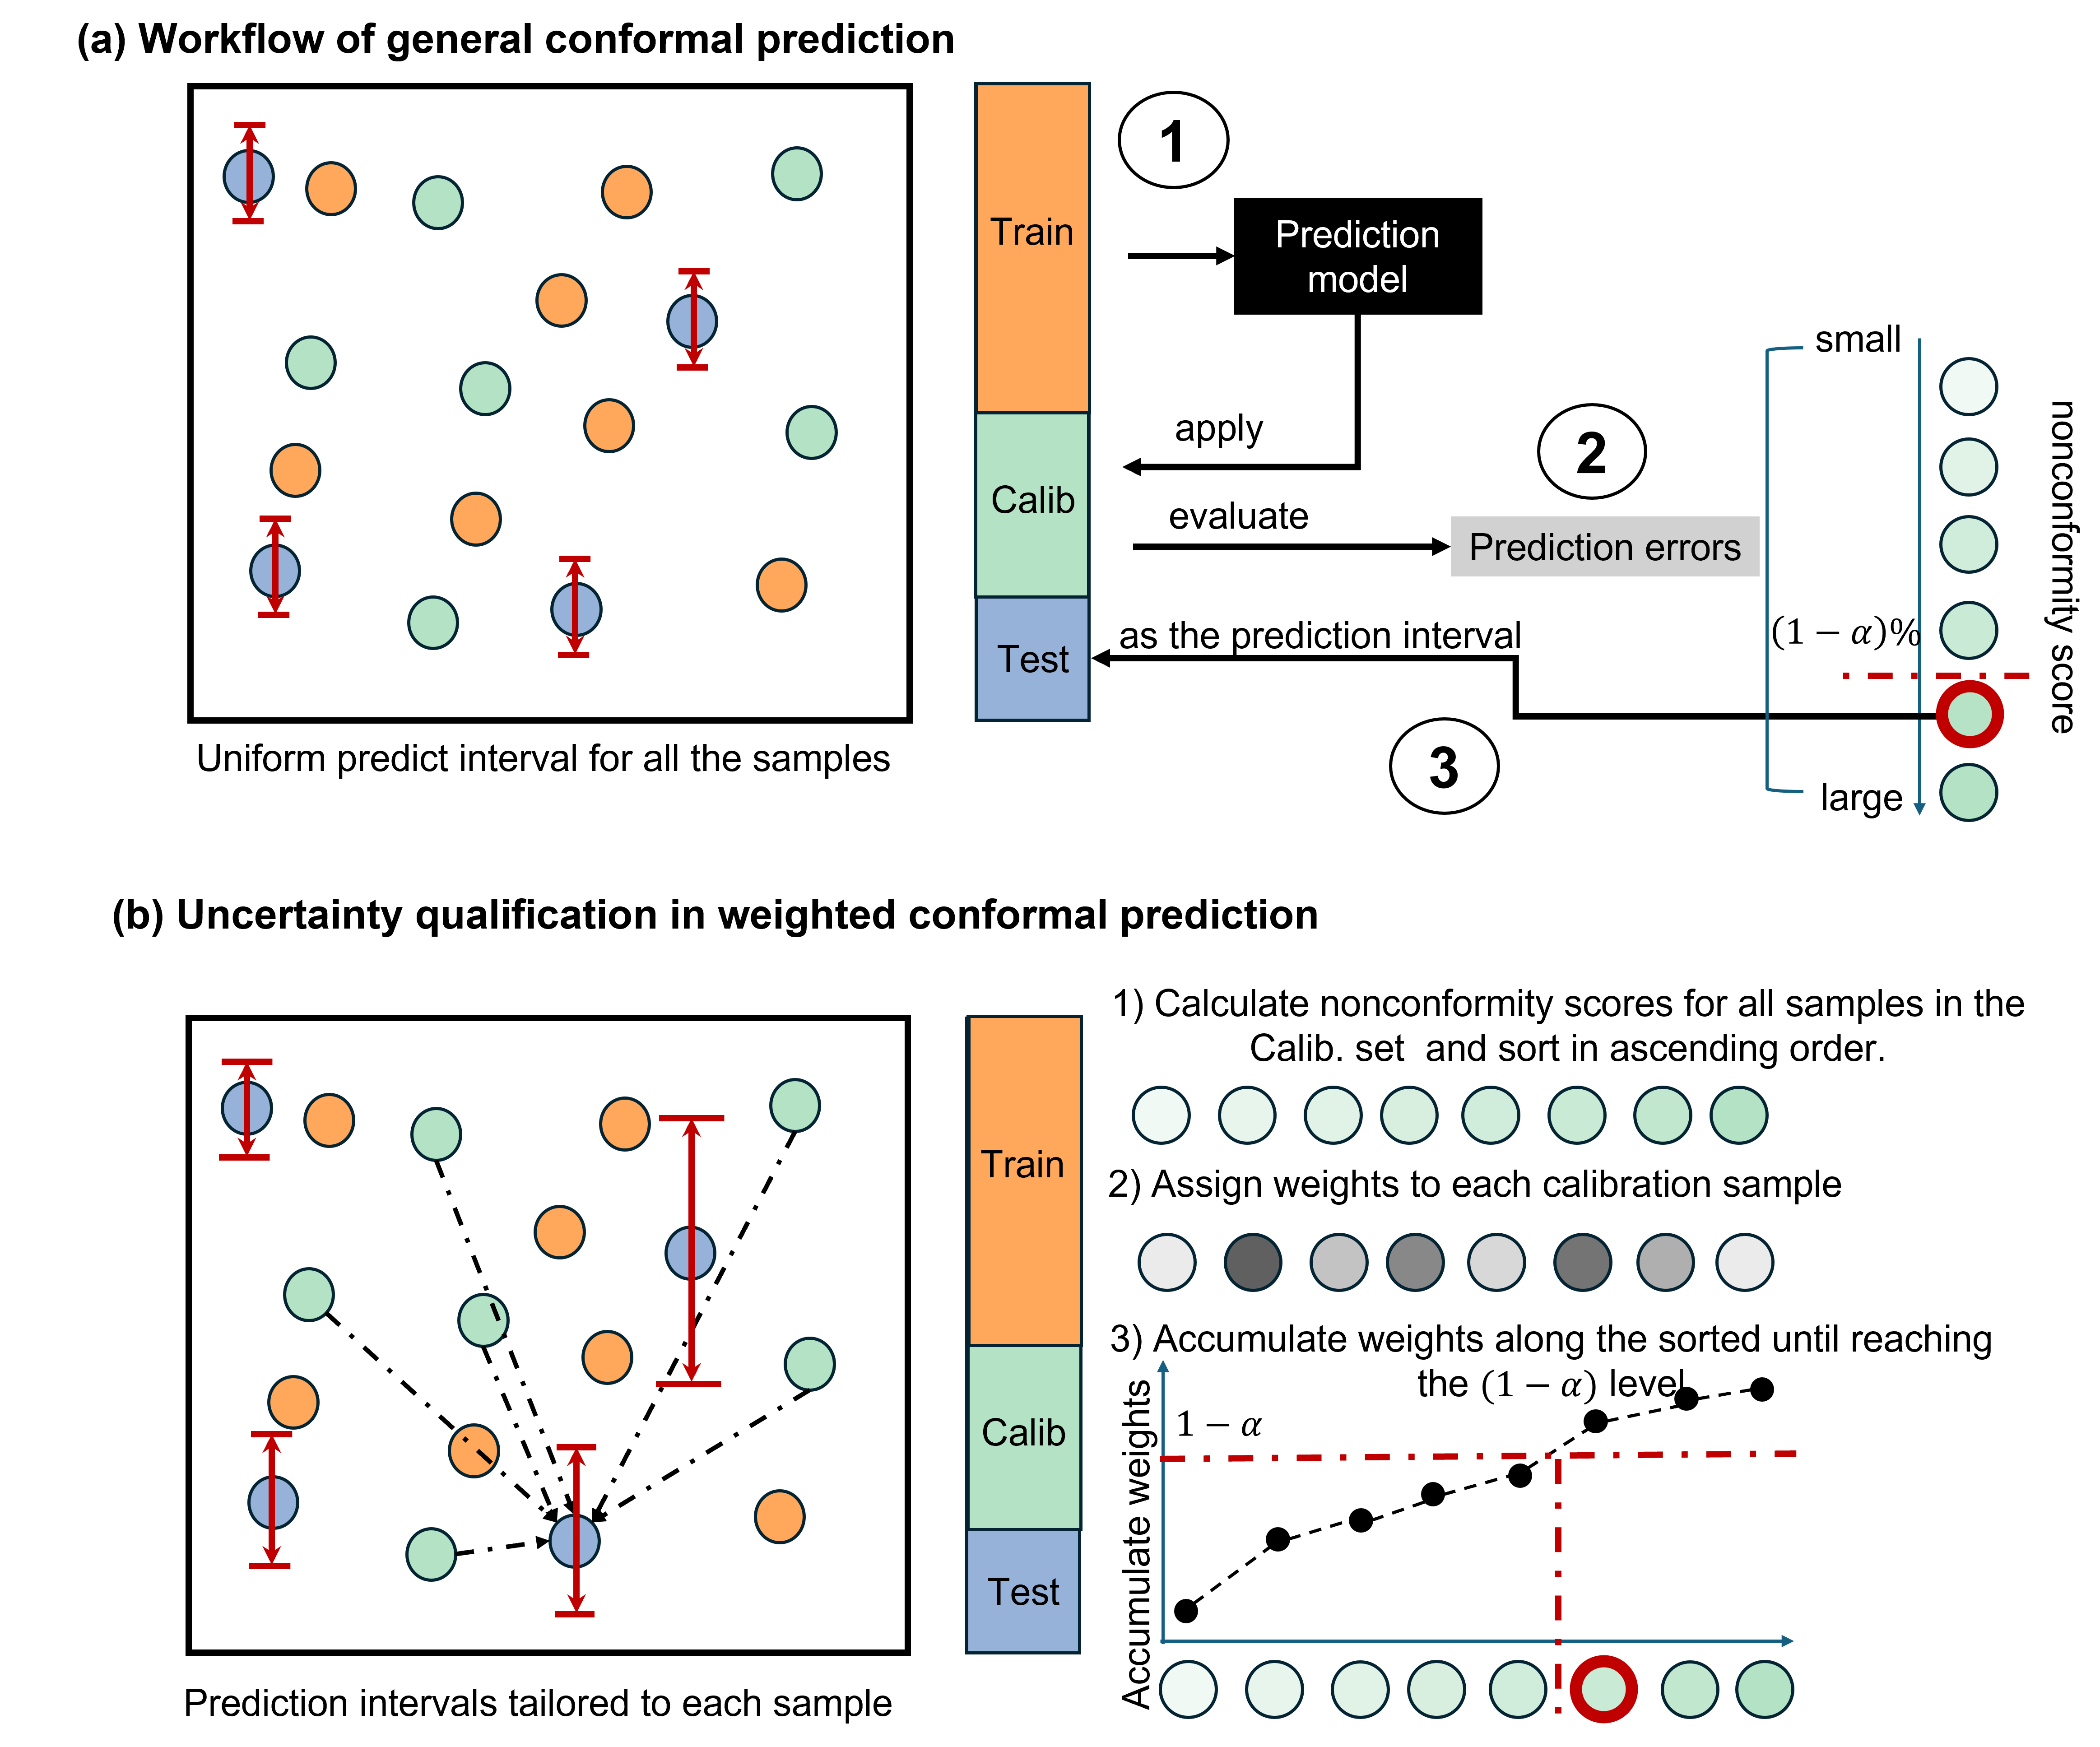
\includegraphics[width=1\linewidth]{Figures/FigureX_concept_of_GeoCP.png}
    \caption{Workflow and concept of conformal prediction in spatial setting}
    \label{fig:framework_geocp}
\end{figure*}




\subsection{Conformal prediction in spatial context}

\subsubsection{Geographic Weighting in GeoCP}

To mitigate covariate shift in spatial prediction tasks, GeoCP was developed by incorporating the idea of WCP with a geographic weighting mechanism grounded in Tobler’s First Law of Geography \citep{tobler2004first}, i.e. \textit{Everything is related to everything else, but near things are more related than distant things.} 

GeoCP leverages geographic proximity to assign weights to calibration points. Formally, the weight assigned to a calibration sample $X_i$ is defined as
\begin{equation}
w_i(u_{\text{test}}, v_{\text{test}}) = K\!\left( \frac{d_{\text{geo}}(i, (u_{\text{test}}, v_{\text{test}}))}{b} \right),
\end{equation}
where $d_{\text{geo}}(i, (u_{\text{test}}, v_{\text{test}}))$ is the geographic distance between the test point and the $i$-th calibration point, $K(\cdot)$ is a smoothing kernel (e.g., Gaussian), and $b$ is the bandwidth controlling the decay rate. 

The prediction set at location $(u_{\text{test}}, v_{\text{test}})$ is then
\begin{equation}
C_{\text{geo}}(X_{\text{test}}) = \Big\{ y \in \mathcal{Y} : \alpha(f(X_{\text{test}}), y) \leq q_{1-\epsilon}^{(\text{geo})}(u_{\text{test}}, v_{\text{test}}) \Big\},
\end{equation}
where the geographically weighted quantile is defined as
\begin{equation}
q_{1-\epsilon}^{(\text{geo})}(u_{\text{test}}, v_{\text{test}}) := \inf \left\{ t : \frac{\sum_{i=1}^m w_i(u_{\text{test}}, v_{\text{test}}) \cdot \mathbb{I}(\alpha_i \leq t)}{\sum_{i=1}^m w_i(u_{\text{test}}, v_{\text{test}})} \geq 1-\epsilon \right\}.
\end{equation}

This geographically-informed weighting scheme serves as a proxy for the covariate likelihood ratio in weighted conformal prediction. It enables the construction of location-specific prediction intervals that adapt to local spatial structure. In effect, it restores a form of \emph{localized weighted exchangeability}, allowing the conformal framework to remain valid in spatially heterogeneous settings. This approach is particularly valuable in scenarios where explanatory variables are scarce or unavailable. For example, in spatial interpolation tasks such as mineral content mapping, the model inputs may consist only of spatial coordinates and mineral content values. In such cases, geographical distance serves as the most reliable metric for evaluating statistical similarity between test points and calibration points, thereby enabling the mitigation of covariate shift.

%feature-based similarity cannot be reliably computed, and conformal methods relying on covariates would fail to provide meaningful uncertainty estimates. Moreover, feature-based weighting may be sensitive to the choice of variables or inconsistent across datasets, reducing robustness and generalizability.

By relying purely on geographic locations to generate weights, GeoCP provides a unified framework for spatial uncertainty quantification across different models and datasets. In doing so, it also reflects the intrinsic spatial structure of geographic data, where observations closer in space tend to exhibit similar behavior.



% To mitigate covariate shift in spatial prediction tasks, GeoCP was developed by incorporating the idea of WCP with a geographic weighting mechanism grounded in Tobler’s First Law of Geography, i.e. \textit{Everything is related to everything else, but near things are more related than distant things.} 

% GeoCP leverages geographic proximity to assign weights to calibration points. Formally, the weight assigned to a calibration sample $X_i$ is defined as
% \begin{equation}
% w_i(u_{\text{test}}, v_{\text{test}}) = K\!\left( \frac{d_{\text{geo}}(i, (u_{\text{test}}, v_{\text{test}}))}{b} \right),
% \end{equation}
% where $d_{\text{geo}}(i, (u_{\text{test}}, v_{\text{test}}))$ is the geographic distance between the test point and the $i$-th calibration point, $K(\cdot)$ is a smoothing kernel (e.g., Gaussian or tricube), and $b$ is the bandwidth controlling the decay rate. The prediction set at location $(u_{\text{test}}, v_{\text{test}})$ is then
% \begin{equation}
% C_{\text{geo}}(X_{\text{test}}) = \Big\{ y \in \mathcal{Y} : \alpha(f(X_{\text{test}}), y) \leq q_{1-\epsilon}^{(\text{geo})}(u_{\text{test}}, v_{\text{test}}) \Big\},
% \end{equation}
% where the geographically weighted quantile is defined as
% \begin{equation}
% q_{1-\epsilon}^{(\text{geo})}(u_{\text{test}}, v_{\text{test}}) := \inf \left\{ t : \frac{\sum_{i=1}^m w_i(u_{\text{test}}, v_{\text{test}}) \cdot \mathbb{I}(\alpha_i \leq t)}{\sum_{i=1}^m w_i(u_{\text{test}}, v_{\text{test}})} \geq 1-\epsilon \right\}.
% \end{equation}


% This geographically-informed weighting scheme serves as a proxy for the covariate likelihood ratio in weighted conformal prediction. It enables the construction of location-specific prediction intervals that adapt to local spatial structure. In effect, it restores a form of \emph{localized weighted exchangeability}, allowing the conformal framework to remain valid in spatially heterogeneous settings.

% This approach is particularly valuable in scenarios where explanatory variables are scarce or unavailable. For instance, in spatial interpolation tasks such as mineral content mapping, model inputs may consist solely of spatial coordinates $\{(u_i, v_i)\}_{i=1}^n$ and scalar values $\{z_i\}_{i=1}^n$. In such cases, feature-based similarity cannot be reliably computed, and conformal methods relying on covariates would fail to provide meaningful uncertainty estimates. Moreover, feature-based weighting may be sensitive to the choice of variables or inconsistent across datasets, reducing robustness and generalizability.

% By relying purely on geographic locations to generate weights, GeoCP provides a \textbf{unified and transferable framework} for spatial uncertainty quantification across different models and datasets. In doing so, it also reflects the intrinsic spatial structure of geographic data, where observations closer in space tend to exhibit similar behavior.

% The prediction interval at a test location $(u_{\text{test}}, v_{\text{test}})$ is constructed as:
% \begin{equation}
% \mathbb{P}[y_{\text{test}} \in C_{\text{geo}}(X_{\text{test}}) \mid (u_{\text{test}}, v_{\text{test}})] \geq 1 - \epsilon,
% \end{equation}
% where the prediction region is defined as:
% \begin{equation}
% C_{\text{geo}}(X_{\text{test}}) = \left\{ y : \alpha(f(X_{\text{test}}), y) \leq \operatorname{GeoQuantile}_{1 - \epsilon}(u_{\text{test}}, v_{\text{test}}; \alpha_1, \dots, \alpha_m) \right\},
% \end{equation}
% and the geographically weighted quantile is computed by:
% \begin{equation}
% \operatorname{GeoQuantile}_{1 - \epsilon}(u_{\text{test}}, v_{\text{test}}; \alpha_1, \dots, \alpha_m) = \operatorname{Quantile}_{1 - \epsilon} \left( \sum_{i=1}^m w_i(u_{\text{test}}, v_{\text{test}}) \cdot \delta_{\alpha_i} \right).
% \end{equation}

% Here, $w_i(u_{\text{test}}, v_{\text{test}})$ denotes the geographic weight assigned to the $i$-th calibration sample relative to the test location, and $\delta_{\alpha_i}$ is a point mass centered at the nonconformity score $\alpha_i$. 

\vspace{0.5em}



\subsubsection{Incorporating feature similarity to deal with spatial nonstationary process}

As mentioned earlier, one of the key motivations and application domains of GeoCP lies in spatial prediction tasks where high-quality explanatory variables are unavailable. In such cases, the model relies solely on spatial distance to assess distributional similarity between locations—this defines the specific setting of GeoCP. However, relying purely on geographic proximity presents limitations. In some cases, geographically close samples can exhibit substantial differences in covariate values, meaning that spatial proximity alone often fails to capture complex spatial processes in heterogeneous regions. This phenomenon is commonly referred to as a spatially nonstationary process. For example, in housing price prediction, two apartments in adjacent communities may follow different statistical distributions if they belong to distinct land-use types—such as one in a residential zone and the other in a commercial district. \textcolor{red}{In such cases, GeoCP’s assumption of local exchangeability—based solely on geospatial proximity—may be violated. Accurately characterizing similarity in the response variable distribution requires accounting for both geographic distance and covariate similarity.}

To address this challenge, we aim to enhance GeoCP for spatial prediction tasks where high-quality explanatory variables are available. Prior studies have highlighted that feature similarity—the degree to which two locations share both spatial context and covariate characteristics—is often a more reliable indicator of underlying process similarity than geographic proximity alone, particularly in spatially nonstationary settings \citep{zhu2022third,luo2024generalized}. Research findings on geographic similarity have been applied to improve various spatial analysis tasks by developing more accurate measures of similarity between locations that go beyond simple geographic distance. These enhanced similarity metrics have led to improved performance in both spatial prediction \citep{zhao2023spatial} and spatial pattern recognition \citep{zhao2025multivariate}.

Inspired by prior studies on geographic similarity, we propose GeoSIMCP, an extension of GeoCP that combines feature-space distance and geographic distance to measure the statistical similarity between locations across space. The details of the GeoSIMCP framework are presented in Section~\ref{sec:geosimcp}.





\subsection{Methodology of GeoSIMCP}
\label{sec:geosimcp}


The motivation behind GeoSIMCP is to jointly consider both spatial and covariate-based similarities, enabling the model to adapt to spatial nonstationarity by incorporating both geographic proximity and feature similarity. GeoSIMCP defines a composite similarity metric between each calibration point and the test point using a \emph{joint distance}:
\begin{equation}
d_{\text{joint}}(i) = \sqrt{ \lambda \cdot d_{\text{geo}}(i)^2 + (1 - \lambda) \cdot d_{\text{feat}}(i)^2 },
\end{equation}
where $d_{\text{geo}}(i)$ is the geographic distance (e.g., Euclidean or geodesic), $d_{\text{feat}}(i)$ is the feature-space distance, and $\lambda \in [0,1]$ controls the trade-off between spatial and attribute information. \textcolor{red}{This linear combination is a pragmatic design choice balancing computational efficiency with interpretability. Thus, the joint distance acts as a heuristic similarity measure to operationalize the localized joint weighted exchangeability—the theoretical cornerstone of GeoSIMCP. Formally, the trade-off parameter $\lambda$ is not a physical spatial property (e.g., spatial autocorrelation) but a functional parameter to optimize local exchangeability. By tuning $\lambda$, the framework identifies the optimal neighborhood of calibration residuals, ensuring uncertainty estimates remain statistically valid and adaptive to nonstationary environments.}



GeoSIMCP supports multiple formulations of $d_{\text{feat}}(i)$ depending on the characteristics of the data. The feature inputs are first standardized using z-score normalization to ensure compatibility between distance magnitudes. In contrast, the geographic coordinates are not standardized, as their spatial distances inherently carry physical meaning in real-world units (e.g., kilometers). We assume that the influence of scale differences between the spatial and feature distances can be reasonably mitigated through the adjustable weighting parameter.

In this study, we propose two basic types of feature distance ($d_{\text{feat}}$) considered in GeoSIMCP. For the $i$-th calibration sample, the first type of distance is Euclidean Distance (EUD):
\begin{equation}
d_{\text{EUC}}(i)  = | X_i - X_{\text{test}} |2,
\end{equation}
where both $X_i$ and $X{\text{test}}$ can be optionally standardized (e.g., z-score normalized) to ensure comparability across dimensions.

% The second type of distance is Minimum Normalized Difference (MND):
% \begin{equation}
% \tilde{d}{\text{feat}}^{(j)} = \frac{|X_i^{(j)} - X{\text{test}}^{(j)}|}{\text{range}(X^{(j)})}, \quad d_{\text{feat}}^{\text{min}}(i) = 1 - \min_j \left(1 - \tilde{d}_{\text{feat}}^{(j)}\right),
% \end{equation}
% where feature ranges are precomputed on the calibration set. This formulation emphasizes the least similar attribute dimension, which can be more robust in settings with dominant local features or heteroskedastic attributes.

The second type of distance is Minimum Normalized Difference (MND):
\begin{equation}
d_{\text{MND}}(i) = 1 - \min_{j = 1, \dots, p} \left(1 - \frac{|X_i^{(j)} - X_{\text{test}}^{(j)}|}{\max_i X_i^{(j)} - \min_i X_i^{(j)}}\right)
\label{eq:mnd_direct}
\end{equation}
Here, $X_i^{(j)}$ denotes the value of the $j$-th feature for the $i$-th calibration sample, and $X_{\text{test}}^{(j)}$ is the corresponding value for the test sample. The index $j \in \{1, 2, \dots, p\}$ ranges over all $p$ feature dimensions. 

This normalization ensures that all feature differences are scaled to the $[0,1]$ interval. The overall MND distance $d_{\text{MND}}(i)$ is constructed to emphasize the least similar feature dimension between the test and calibration samples. By applying a \textit{minimum} operator to the feature-wise similarities, this formulation captures the intuition that a strong dissimilarity in any single dimension should significantly reduce the overall similarity score. 


The final conformal weights are computed using a kernel smoothing function applied to the joint distance:
\begin{equation}
w_i^{\text{joint}} = \frac{K\left( \dfrac{d_{\text{joint}}(i)}{b} \right)}{\sum_{j=1}^m K\left( \dfrac{d_{\text{joint}}(j)}{b} \right)},
\end{equation}
where $K(\cdot)$ is a smoothing kernel, and $b$ is a bandwidth parameter controlling local sensitivity. \textcolor{red}{While the weighting function in GeoSIMCP is not restricted to a specific form, all experiments in this study consistently employed a Gaussian kernel as the smoothing function to map joint distances to calibration weights. This choice aligns with the default configuration of GeoCP and facilitates fair comparisons across methods \citep{lou2025geoconformal}.}

Using these weights, the prediction interval for a new input $X_{\text{test}}$ is defined as:
\begin{equation}
C_{\text{sim}}(X_{\text{test}}) = \left\{ y : \alpha(f(X_{\text{test}}), y) \leq \operatorname{Quantile}_{1 - \epsilon}^{\text{joint}}(\alpha_1, \dots, \alpha_m) \right\},
\end{equation}
where the weighted quantile is given by:
\begin{equation}
\operatorname{Quantile}_{1 - \epsilon}^{\text{joint}} := \inf \left\{ t : \sum_{i=1}^m w_i^{\text{joint}} \cdot \mathbb{I}(\alpha_i \leq t) \geq 1 - \epsilon \right\}.
\end{equation}

This formulation generalizes previous spatial conformal prediction methods and satisfies finite-sample coverage guarantees under a relaxed, similarity-weighted exchangeability assumption. When $\lambda = 1$, GeoSIMCP reduces to GeoCP, relying only on spatial proximity. When $\lambda = 0$, the method becomes purely feature-based. For $0 < \lambda < 1$, the prediction interval reflects both geographic and attribute similarity, thereby adapting to complex spatial processes.

By flexibly integrating spatial and feature information, GeoSIMCP provides a unified, interpretable, and transferable solution for conformal uncertainty quantification in spatially heterogeneous environments.
\textcolor{red}{The validity of GeoSIMCP relies on a core assumption of localized joint weighted exchangeability. In the presence of spatial non-stationarity, GeoSIMCP posits that the nonconformity score of a instance is exchangeable with those of the calibration samples only after accounting for their joint proximity in both geographic and feature spaces. More specifically, we assume that the error distribution is locally stable, such that observations that are similar in terms of covariates and spatial location exhibit comparable levels of predictive uncertainty. This joint notion of similarity ensures that the calibration set remains representative of the target location under nonstationary spatial process. A rigorous mathematical formulation of this exchangeability assumption, together with the resulting coverage guarantees, is provided in Appendix A.}


The workflow of GeoSIMCP follows the standard conformal prediction pipeline with local adaptivity. First, a prediction model is trained on the training data. Second, nonconformity scores, such as residuals, are computed on the calibration set using the trained model. Third, for each test point, joint distances are evaluated to assign corresponding weights to calibration samples. Finally, prediction intervals are derived from the weighted quantile of the nonconformity scores. The weighting procedure in GeoSIMCP is detailed in Algorithm \ref{alg:geosimcp}.






\begin{algorithm}[ht]
\caption{GeoSIMCP: Jointly Weighted Conformal Prediction}
\label{alg:geosimcp}
\begin{algorithmic}[1]
\Require Calibration set $\{(X_i, y_i)\}_{i=1}^m$, test point $X_{\text{test}}$, nonconformity scores $\{\alpha_i\}_{i=1}^m$, miscoverage level $\epsilon$, trade-off parameter $\lambda$, bandwidth $b$
\Require Distance functions $d_{\text{geo}}(\cdot)$ and $d_{\text{feat}}(\cdot)$, kernel function $K(\cdot)$
\Ensure Weighted conformal quantile $\hat{q}$ for $X_{\text{test}}$

\For{$i = 1$ to $m$}
    \State Compute geographic distance: $d_i^{\text{geo}} \gets d_{\text{geo}}(X_{\text{test}}, X_i)$
    \State Compute feature-space distance: $d_i^{\text{feat}} \gets d_{\text{feat}}(X_{\text{test}}, X_i)$
    \State Compute joint distance: $d_i^{\text{joint}} \gets \sqrt{\lambda \cdot (d_i^{\text{geo}})^2 + (1 - \lambda) \cdot (d_i^{\text{feat}})^2}$
    \State Compute unnormalized weight: $w_i \gets K\left( \dfrac{d_i^{\text{joint}}}{b} \right)$
\EndFor

\State Normalize weights: $w_i \gets w_i / \sum_{j=1}^m w_j$
\State Sort $\{(\alpha_i, w_i)\}$ in ascending order of $\alpha_i$
\State Compute cumulative weights: $C_i \gets \sum_{j=1}^i w_j$
\State Find smallest $k$ such that $C_k \geq 1 - \epsilon$
\State $\hat{q} \gets \alpha_k$
\State \Return $\hat{q}$
\end{algorithmic}
\end{algorithm}




% \begin{figure*}[htbp]
%     \centering
%     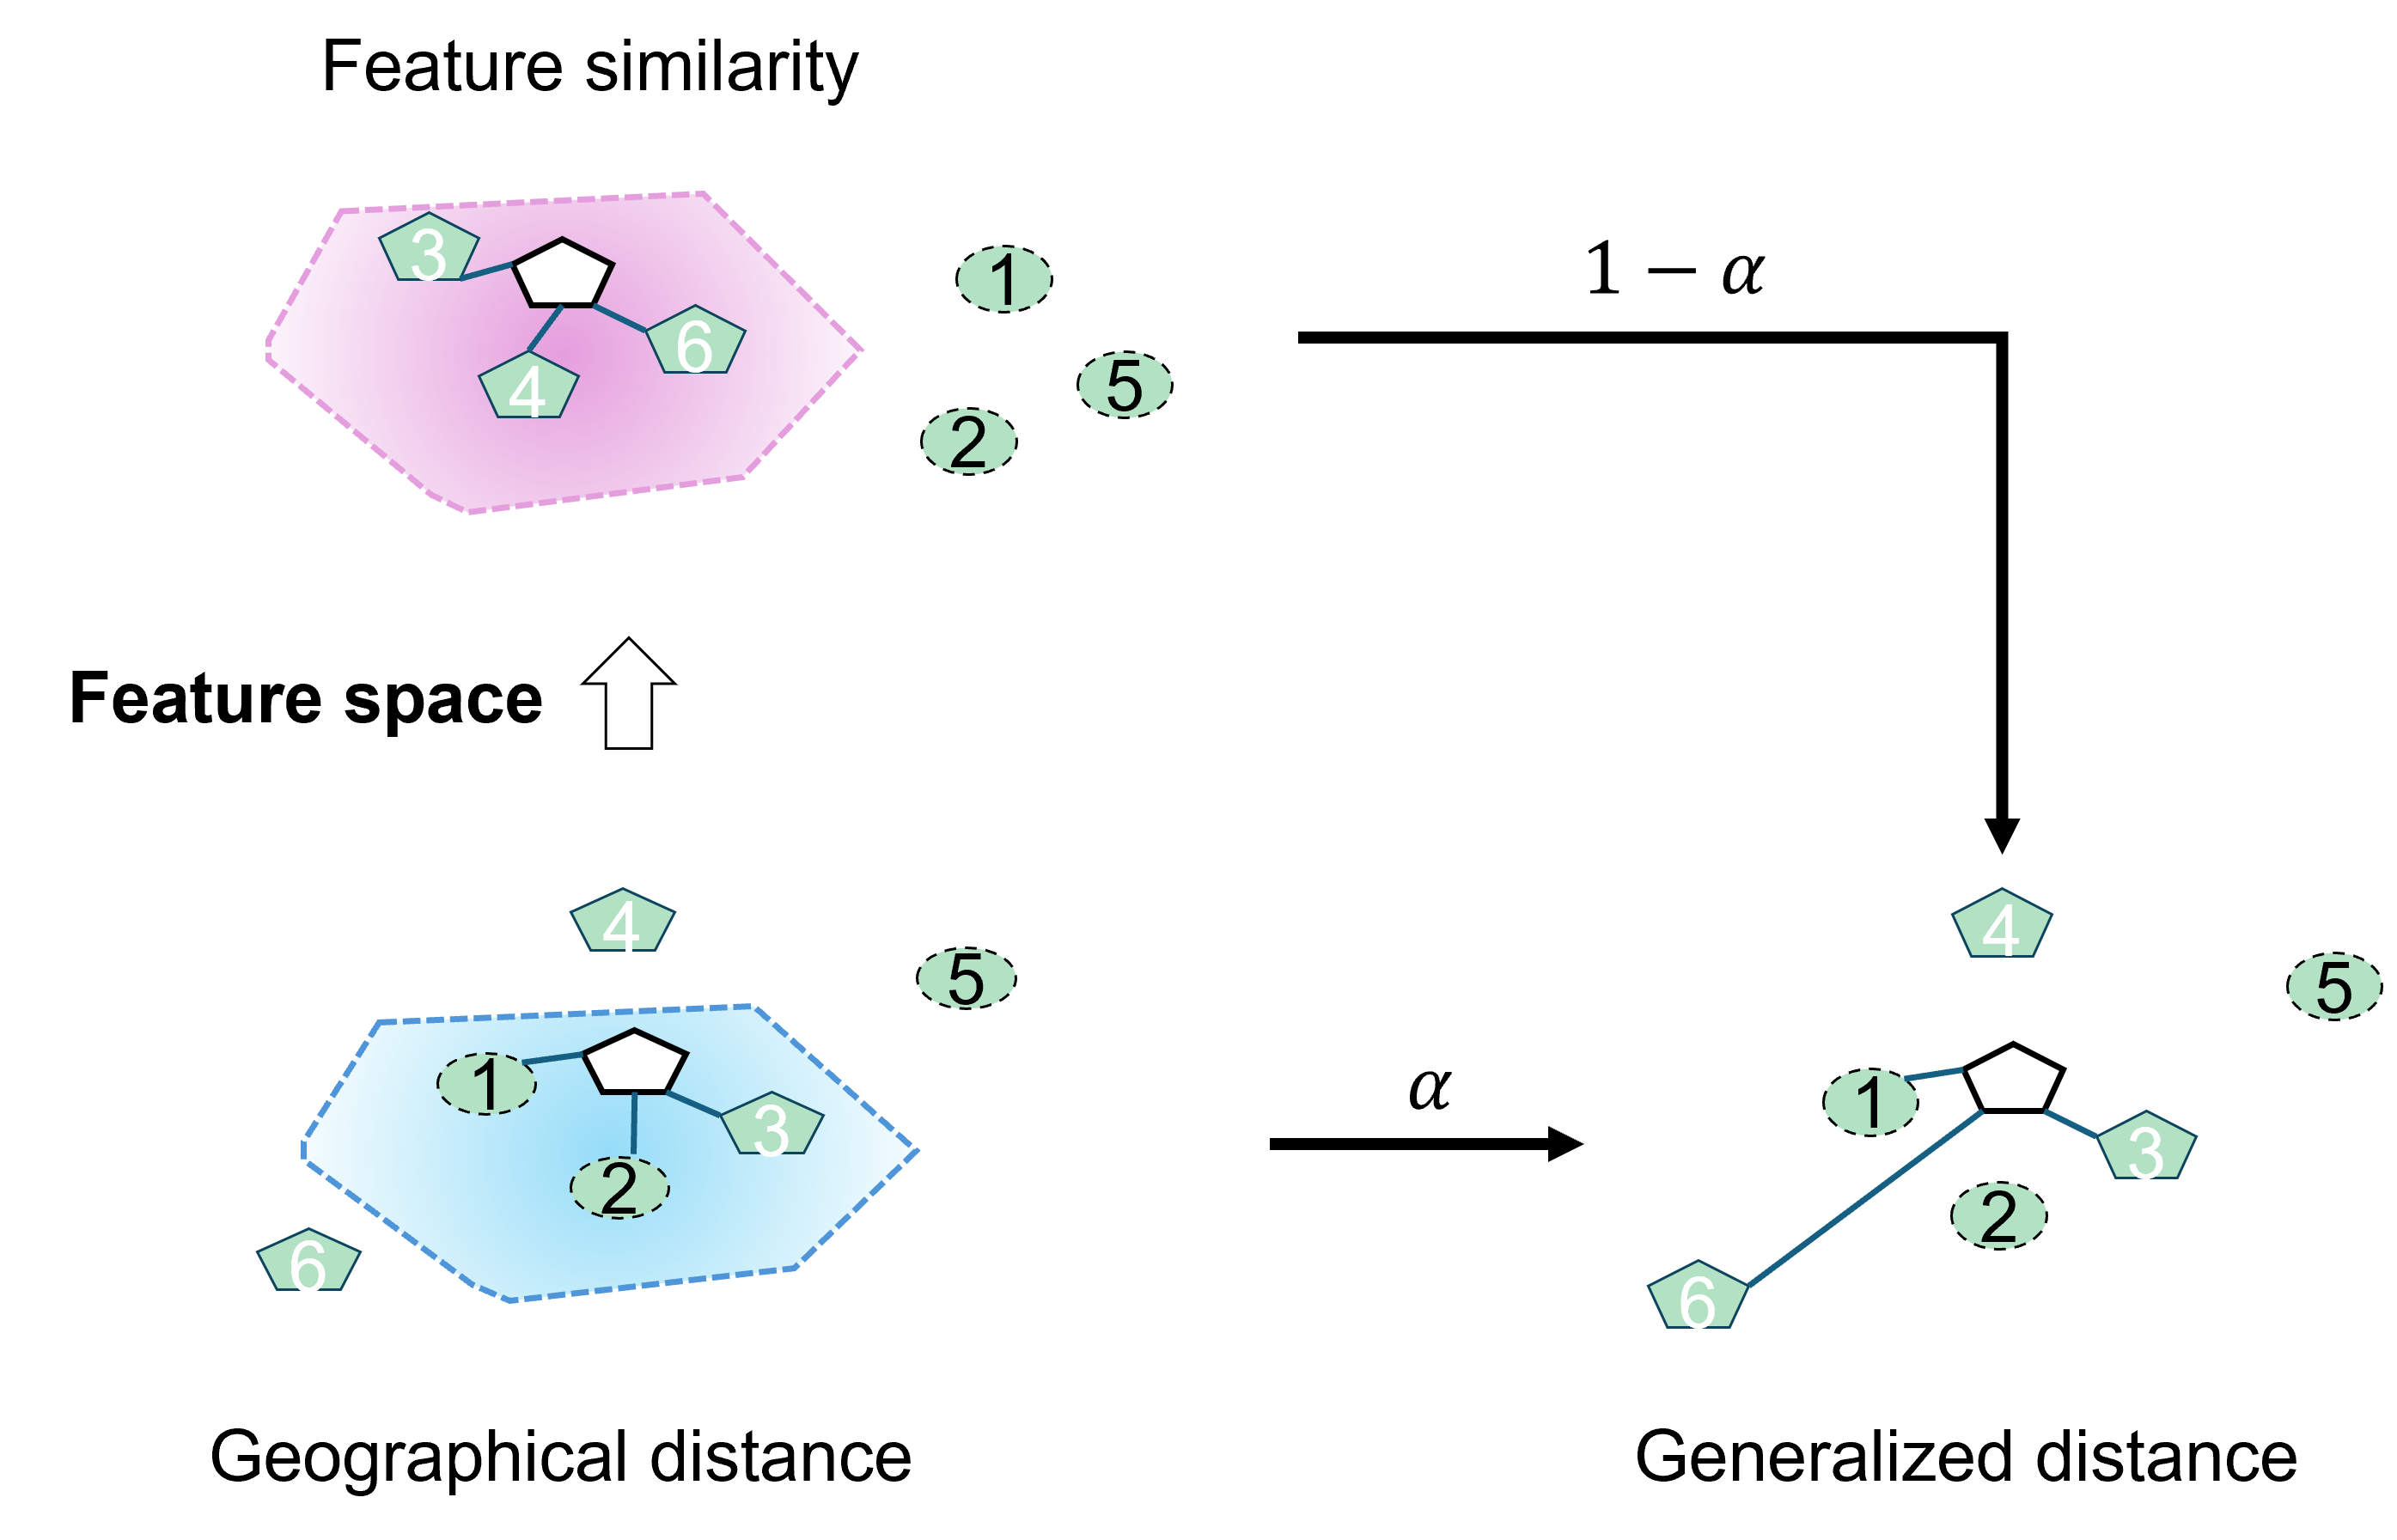
\includegraphics[width=1\linewidth]{Figures/FigureX_feature_weight.png}
%     \caption{Schematic overview of geographic weighting (GeoCP) versus joint feature-geographic weighting (GeoSIMCP).}
%     \label{fig:framework_mlp}
% \end{figure*}

% \subsubsection{Benefits of GeoSIMCP}

% The advantages of GeoSIMCP include:

% \begin{itemize}
%     \item \textbf{Local adaptivity} to both spatial and covariate heterogeneity.
%     \item \textbf{Robustness} to attribute-level covariate shift.
%     \item \textbf{Flexibility} through adjustable \(\lambda\) to balance spatial and feature influences.
% \end{itemize}

\subsection{Hyperparameter optimization}


\textcolor{red}{In both GeoCP and GeoSIMCP, kernel parameters determine how local calibration neighborhoods are constructed and therefore directly influence uncertainty estimation. The bandwidth parameter \(b\) controls the spatial or joint-distance scale over which calibration residuals are aggregated. Smaller values of  \(b\) yield highly localized uncertainty estimates that are more sensitive to fine-scale spatial heterogeneity, but may become unstable when calibration samples are sparse. In contrast, larger values of \(b\) produce smoother and more stable prediction intervals, at the risk of oversmoothing local uncertainty.}

\textcolor{red}{In GeoSIMCP, the trade-off parameter \(\lambda\) further modulates the definition of local exchangeability by balancing geographic proximity and feature-space similarity when characterizing statistical similarity between samples. Unlike parameters that encode physical properties of a spatial process, \(\lambda\) acts as a calibration hyperparameter whose role is to determine which notion of similarity most effectively restores local exchangeability for uncertainty quantification.}

We perform a two-dimensional grid search over bandwidth \(b\) and trade-off parameter \(\lambda\), following the same selection criteria. The optimization follows a two-step procedure. First, we apply a coverage constraint, where only configurations that achieve a coverage above a predefined threshold (e.g., 90\%) are retained. Second, among the models that satisfy this constraint, we select the one with the lowest interval score to ensure both reliability and precision in uncertainty estimation. In uncertainty quantification, the interval score is a comprehensive metric used to evaluate the quality of prediction intervals, balancing the tightness of the interval width and the ability to cover the true value \citep{hofer2022comparing}. Specifically, for the \(i\)-th sample, the interval score is defined as:

\begin{equation}
\begin{aligned}
\text{Interval Score}_i =\ & (\text{Upper}_i - \text{Lower}_i) \\
& + \frac{2}{\alpha} \Big[ (\text{Lower}_i - y_i) \cdot \mathbb{I}(y_i < \text{Lower}_i) \\
& \quad + (y_i - \text{Upper}_i) \cdot \mathbb{I}(y_i > \text{Upper}_i) \Big],
\end{aligned}
\end{equation}

where \(\text{Lower}_i\) and \(\text{Upper}_i\) denote the lower and upper bounds of the predicted interval, \(y_i\) is the ground truth, \(\alpha\) is the significance level (e.g., \(\alpha = 0.1\) for a 90\% prediction interval), and \(\mathbb{I}(\cdot)\) is the indicator function. The first term measures the width of the prediction interval, while the second term penalizes miscoverage—when the true value falls outside the interval. The penalty is inversely proportional to the confidence level, encouraging intervals that are both narrow and well-calibrated. In practice, we replace \((\text{Upper}_i - \text{Lower}_i)\) with \(\max(\text{Upper}_i - \text{Lower}_i, \epsilon)\) to avoid degenerate intervals and ensure numerical stability, where \(\epsilon\) is a small positive constant (e.g., \(10^{-6}\)).




\subsection{Conceptual differences between GeoCP and GeoSIMCP}

%For GeoCP, we perform a grid search over candidate bandwidths \(h\), selecting the one satisfying coverage constraints and minimizing the interval score.

{
\color{red}


\begin{figure*}[htbp]
    \centering
    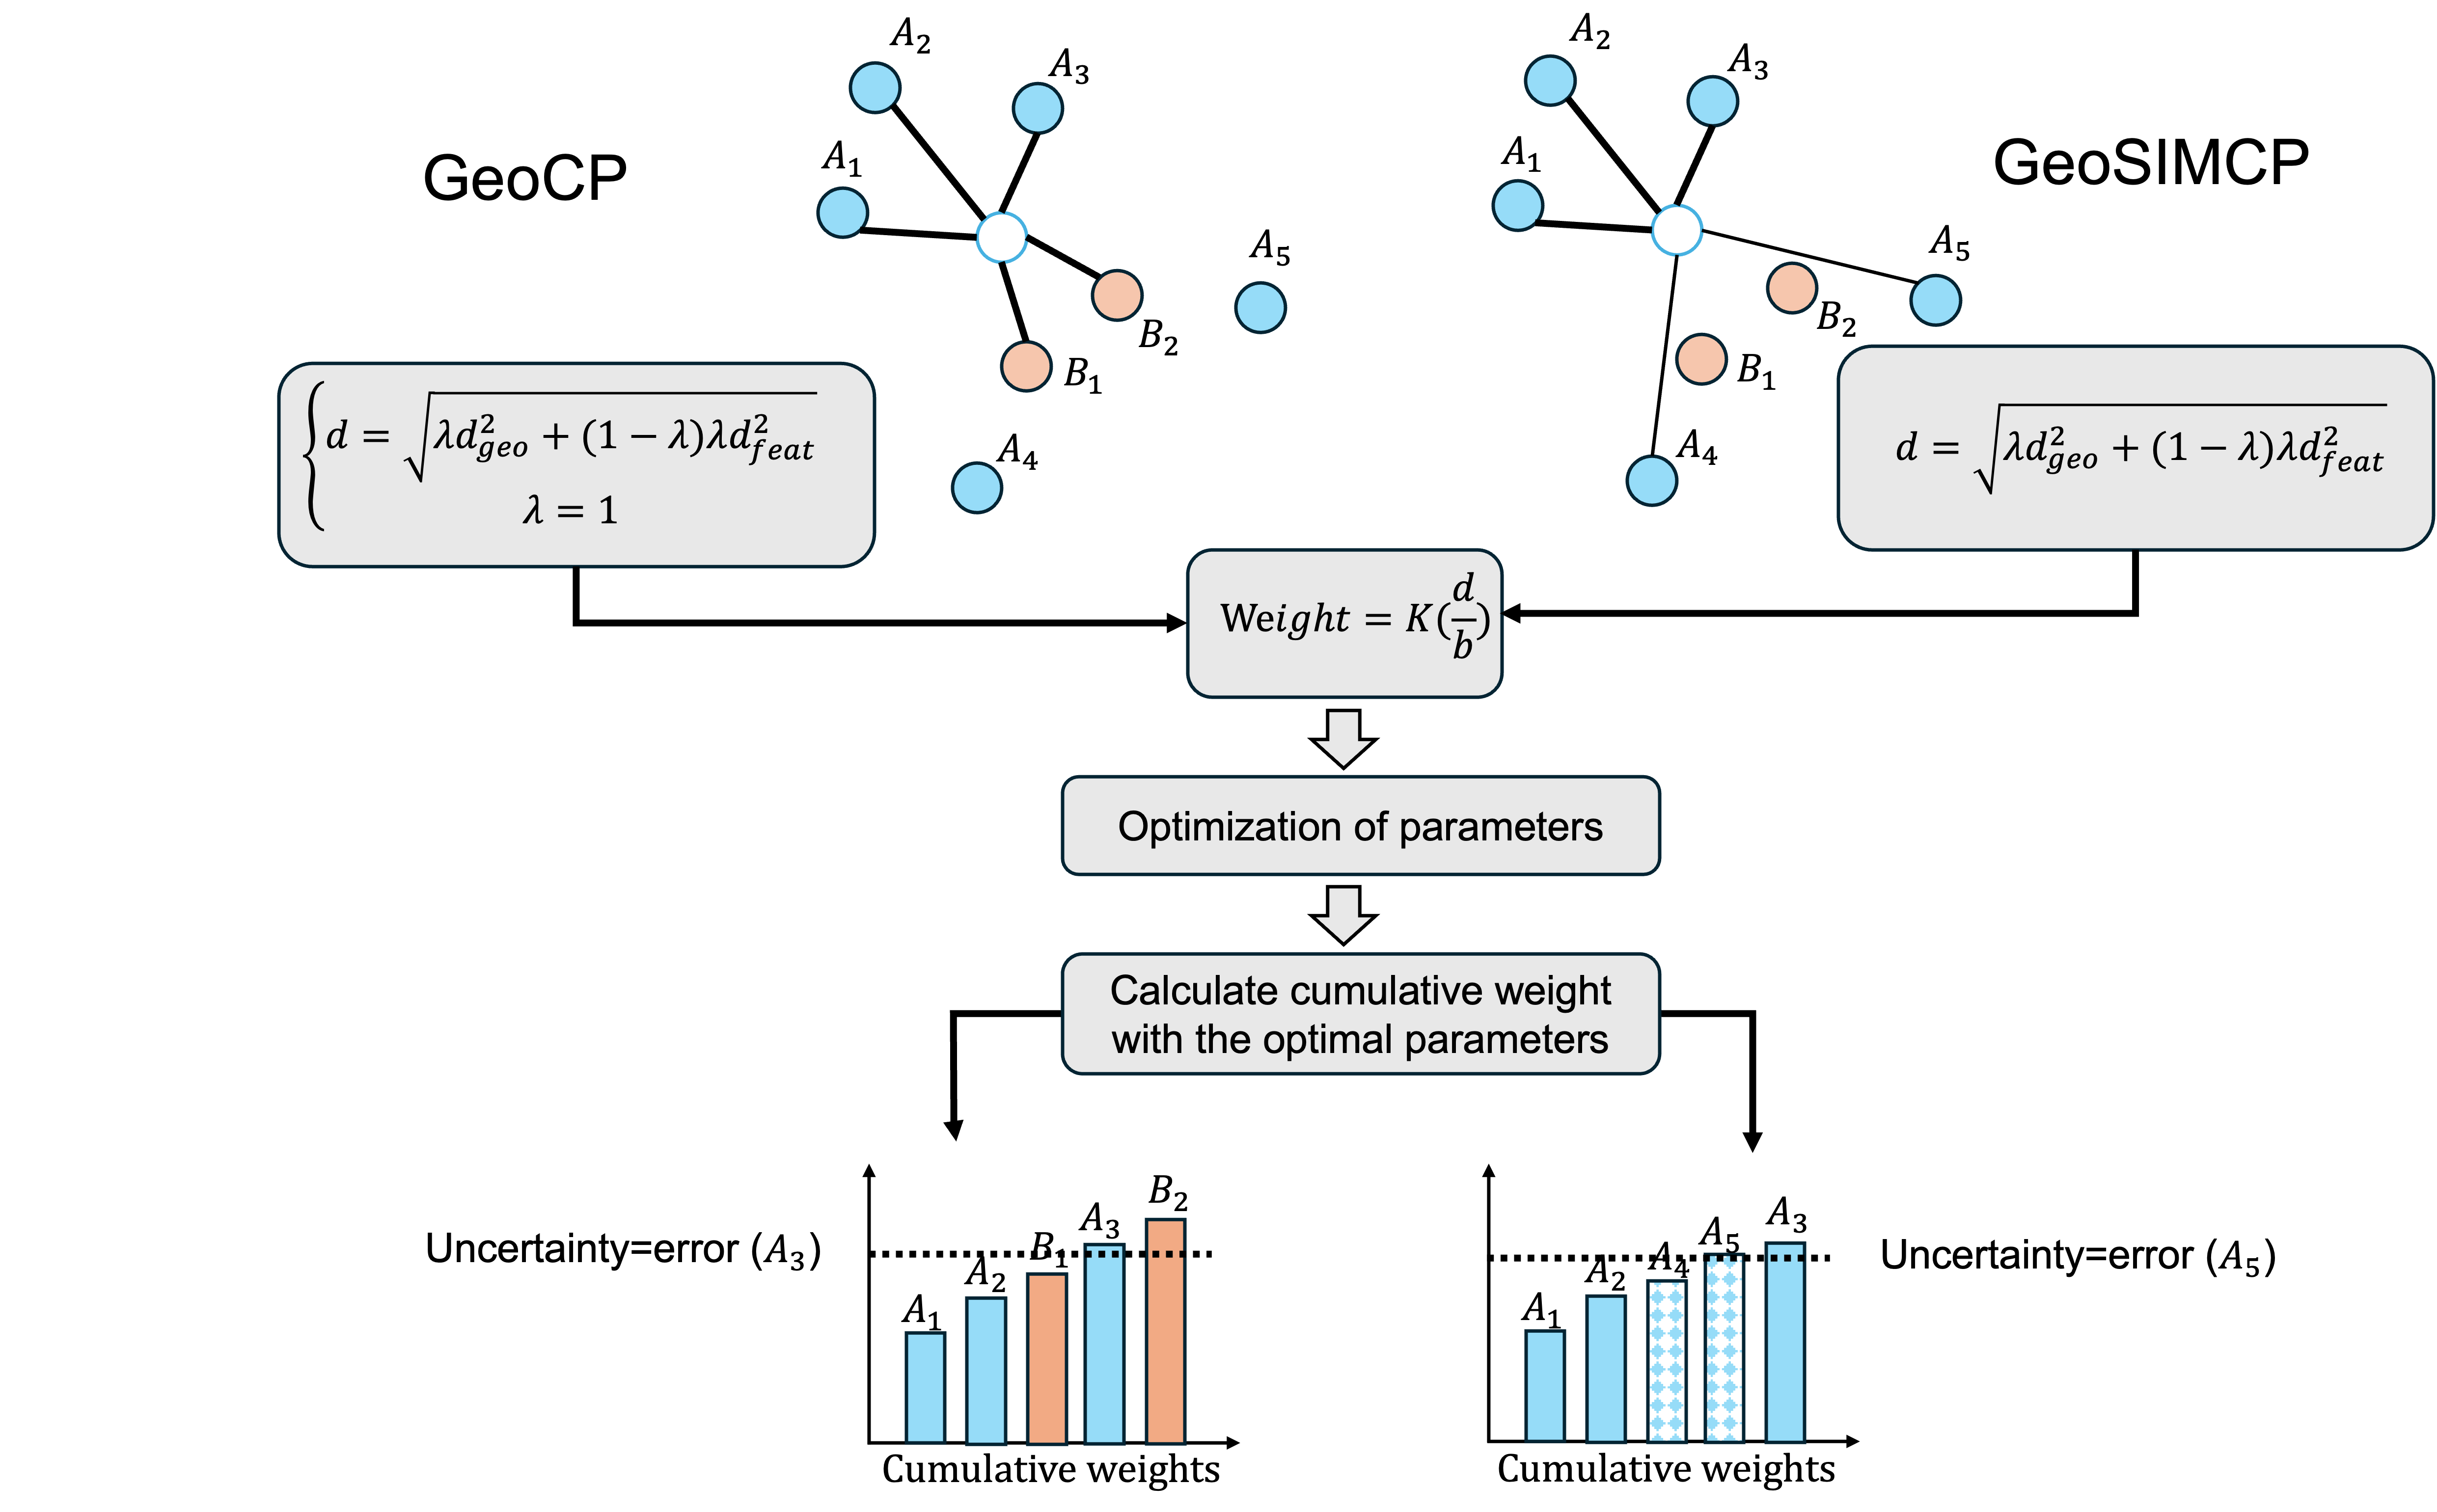
\includegraphics[width=1\linewidth]{Figures/Figure_X_workflow of GeoSIMCP.png}
    \caption{Conceptual illustration of local calibration in GeoCP and GeoSIMCP.}
    \label{fig:geosimcp_workflow}
\end{figure*}
In Figure \ref{fig:geosimcp_workflow}, we illustrate the conceptual differences between GeoSIMCP and GeoCP. Solid points represent calibration samples, for which nonconformity scores with respect to the trained prediction model have been precomputed. We assume that two distinct spatial processes coexist in the region, indicated by blue and orange points. The hollow point denotes a test sample for which predictive uncertainty is to be estimated, and is assumed to originate from the blue spatial process.
To quantify the uncertainty of the test sample, GeoCP relies solely on geographic distance. As a result, calibration samples from a different spatial process (e.g., B1 and B2) may be assigned high weights due to spatial proximity. In contrast, GeoSIMCP incorporates feature-space similarity in addition to geographic distance, allowing calibration samples that are spatially farther but process-consistent (e.g., A4 and A5) to contribute more substantially to local uncertainty estimation.

For both GeoCP and GeoSIMCP, distances between the test sample and all calibration samples are first computed and then transformed into sample weights through a kernel function. An explicit parameter optimization procedure is introduced to identify the optimal parameters governing distance computation and kernel weighting. Specifically, GeoCP optimizes only the kernel bandwidth parameter \(b\) , whereas GeoSIMCP additionally optimizes the parameter \(\lambda\), which controls the trade-off between geographic distance and feature-space distance.


Finally, using the optimal parameters, kernel weights are computed for all calibration samples and aggregated into cumulative weights. Given a user-specified confidence level, these cumulative weights are then used to construct the predictive uncertainty interval for the test sample.




}

\section{Simulation study}


\subsection{True model with simulated uncertainty}


\begin{figure*}[htbp]
    \centering
    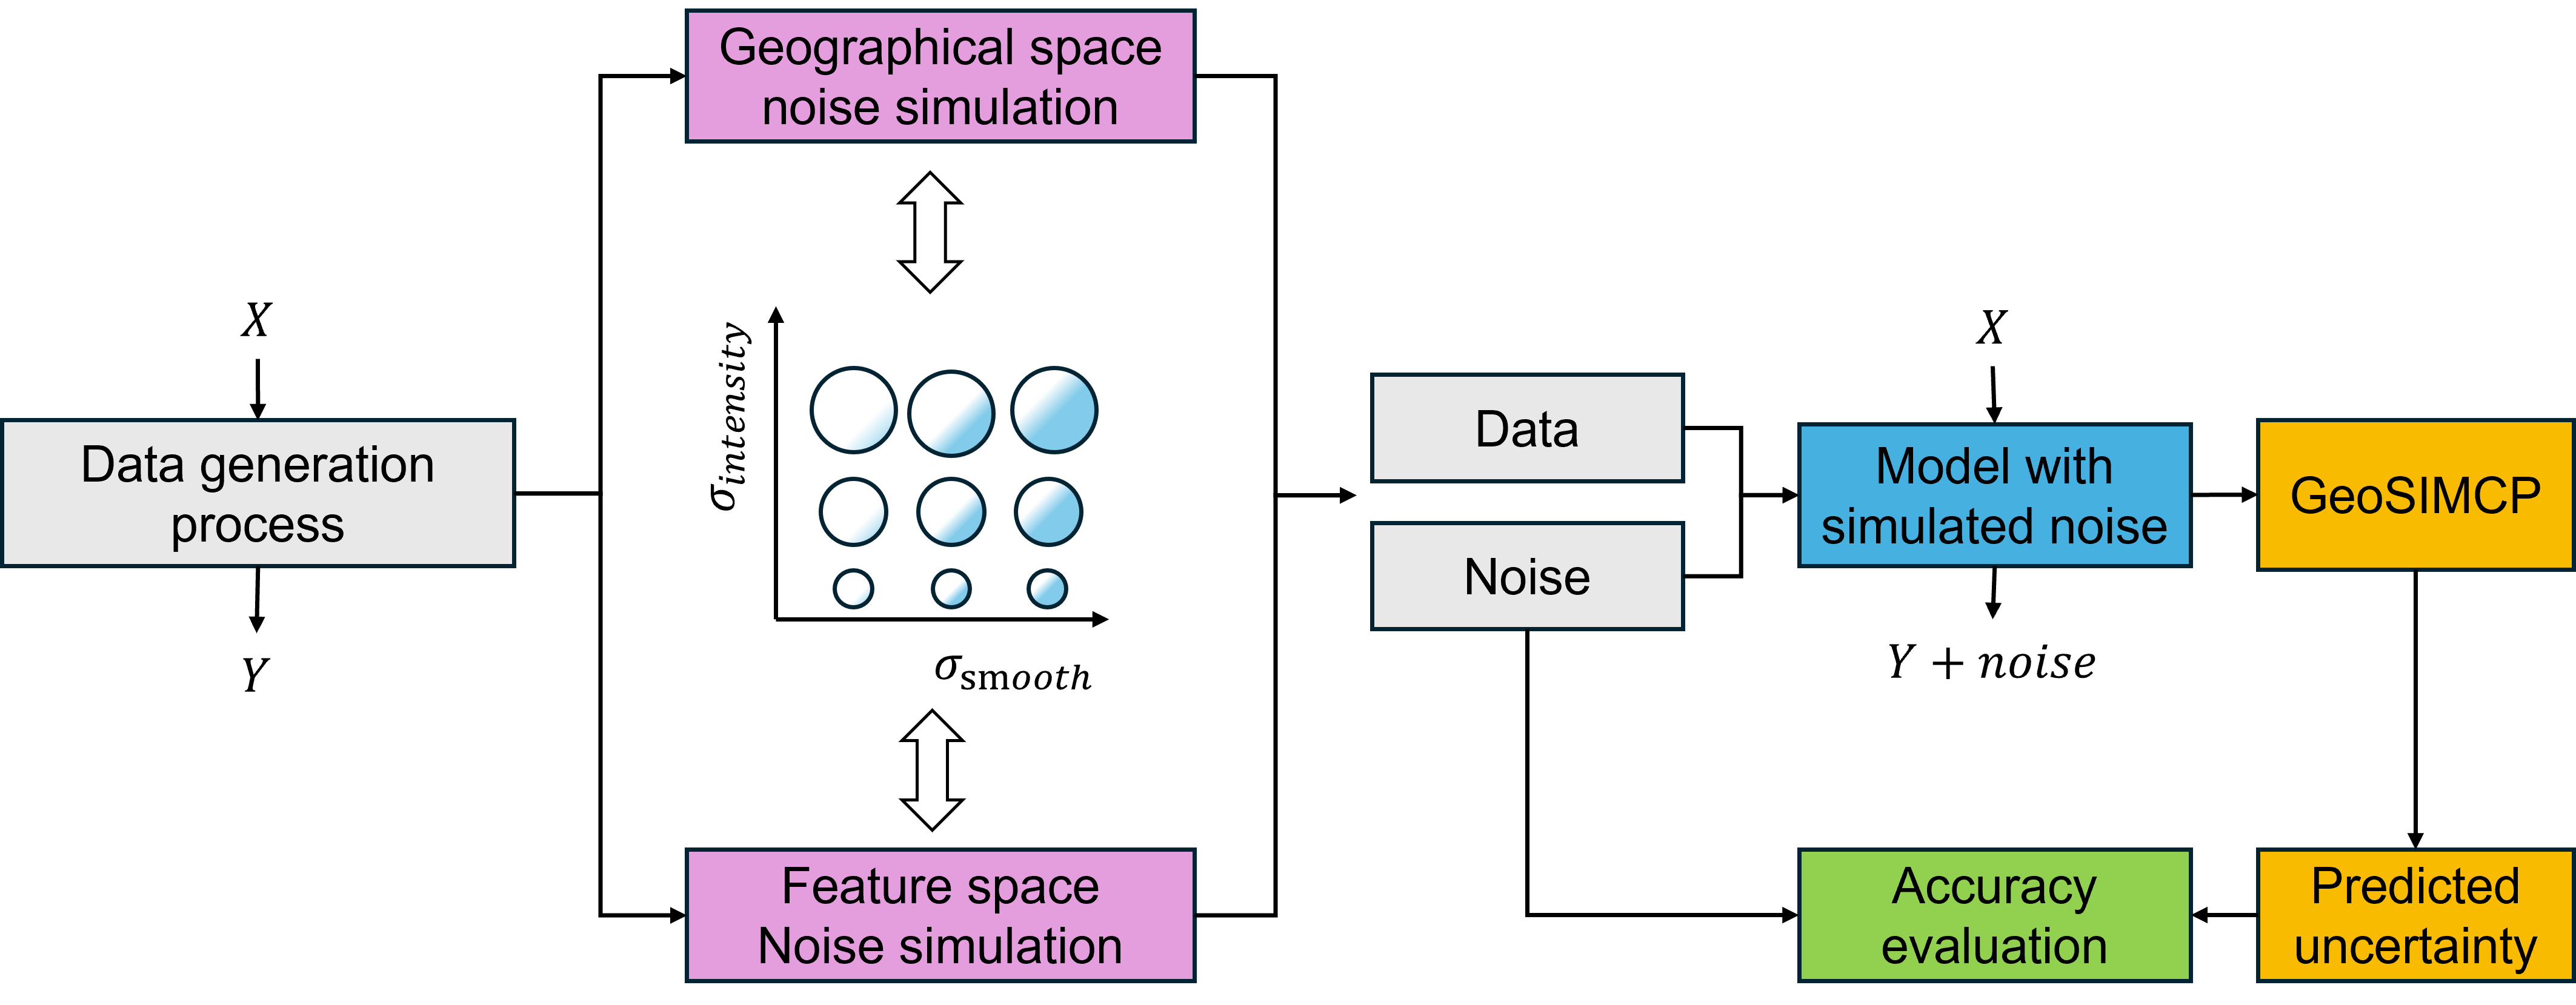
\includegraphics[width=1\linewidth]{Figures/FigureX_simulation_design.png}
    \caption{Workflow of simulation study}
    \label{fig:simu_workflow}
\end{figure*}


{
\color{red}

To evaluate the effectiveness of GeoSIMCP in uncertainty quantification under varying spatial and feature conditions, we conduct simulation experiments for spatial processes with controlled and known uncertainty.

We begin by defining a deterministic data-generating mechanism. Specifically, we assume an underlying structural function
\begin{equation}
D(\cdot): \mathbb{R}^p \rightarrow \mathbb{R},
\end{equation}
which maps the input features to the response. For each spatial unit $i$, given the input feature vector
\begin{equation}
X_i = (X_{1i}, X_{2i}),
\end{equation}
the noise-free outcome is generated as
\begin{equation}
Y_i^{\ast} = D(X_i).
\end{equation}
This function represents the true spatial process and is fixed and known by construction.

Next, stochastic variability is introduced by simulating a location-specific perturbation term. In this study, we consider two types of perturbations: one defined in geographic space and the other defined in feature space. Further details are provided in Section~3.3 and illustrated in Figure~\ref{fig:simu_noise}.

Based on this setup, we define the prediction model as
\begin{equation}
Y_i = D(X_i) + \varepsilon_i,
\end{equation}
where $\varepsilon_i$ denotes the simulated perturbation associated with location $i$. Importantly, the functional relationship between inputs and outputs is exactly the same as the data-generating mechanism. That is, conditional on $X_i$, the prediction model follows the true structural mapping $D(\cdot)$ without approximation or model misspecification.

Under this design, the prediction model constitutes a \emph{true model with simulated uncertainty}. All variability in the predicted response originates from the explicitly simulated perturbation term, while the underlying process remains fixed and known. As a result, the ground-truth predictive uncertainty is well defined and directly traceable to the simulated perturbations.
}
Finally, we apply GeoSIMCP to estimate prediction uncertainty from the simulated data. Since the ground-truth uncertainty is known by construction, this setting enables a quantitative and unambiguous evaluation of GeoSIMCP’s uncertainty quantification performance.





\subsection{Data generation}


A two-dimensional regular grid of size $100\times100$ is created over the $[0,1]\times[0,1]$ domain, with each sample associated with its $(x, y)$ geographic coordinates.
Feature $X_1$ is generated by drawing values from a uniform distribution over $[5, 10]$, followed by spatial smoothing using a Gaussian filter with standard deviation $\sigma=5$. Feature $X_2$ is generated from a uniform distribution over $[0, 6]$ and smoothed with a Gaussian filter of standard deviation $\sigma=1.5$.


The true target variable $Y$ is constructed as:

\begin{equation}
Y = X_1 + X_2,
\end{equation}

where both $X_1$ and $X_2$ exhibit distinct spatial autocorrelation patterns.




\subsection{Noise generation}
\label{sec:noise_generation}

To simulate realistic and heterogeneous uncertainty in spatial modeling, we design a unified noise generation framework that supports multiple spatial structures. All noise values \(\varepsilon\) are ultimately defined over a two-dimensional spatial grid, ensuring that spatial correlation and local variation can be systematically controlled. We implement two types of noise generation mechanisms, each corresponding to a distinct theoretical perspective and real-world interpretation.


\begin{figure*}[htbp]
    \centering
    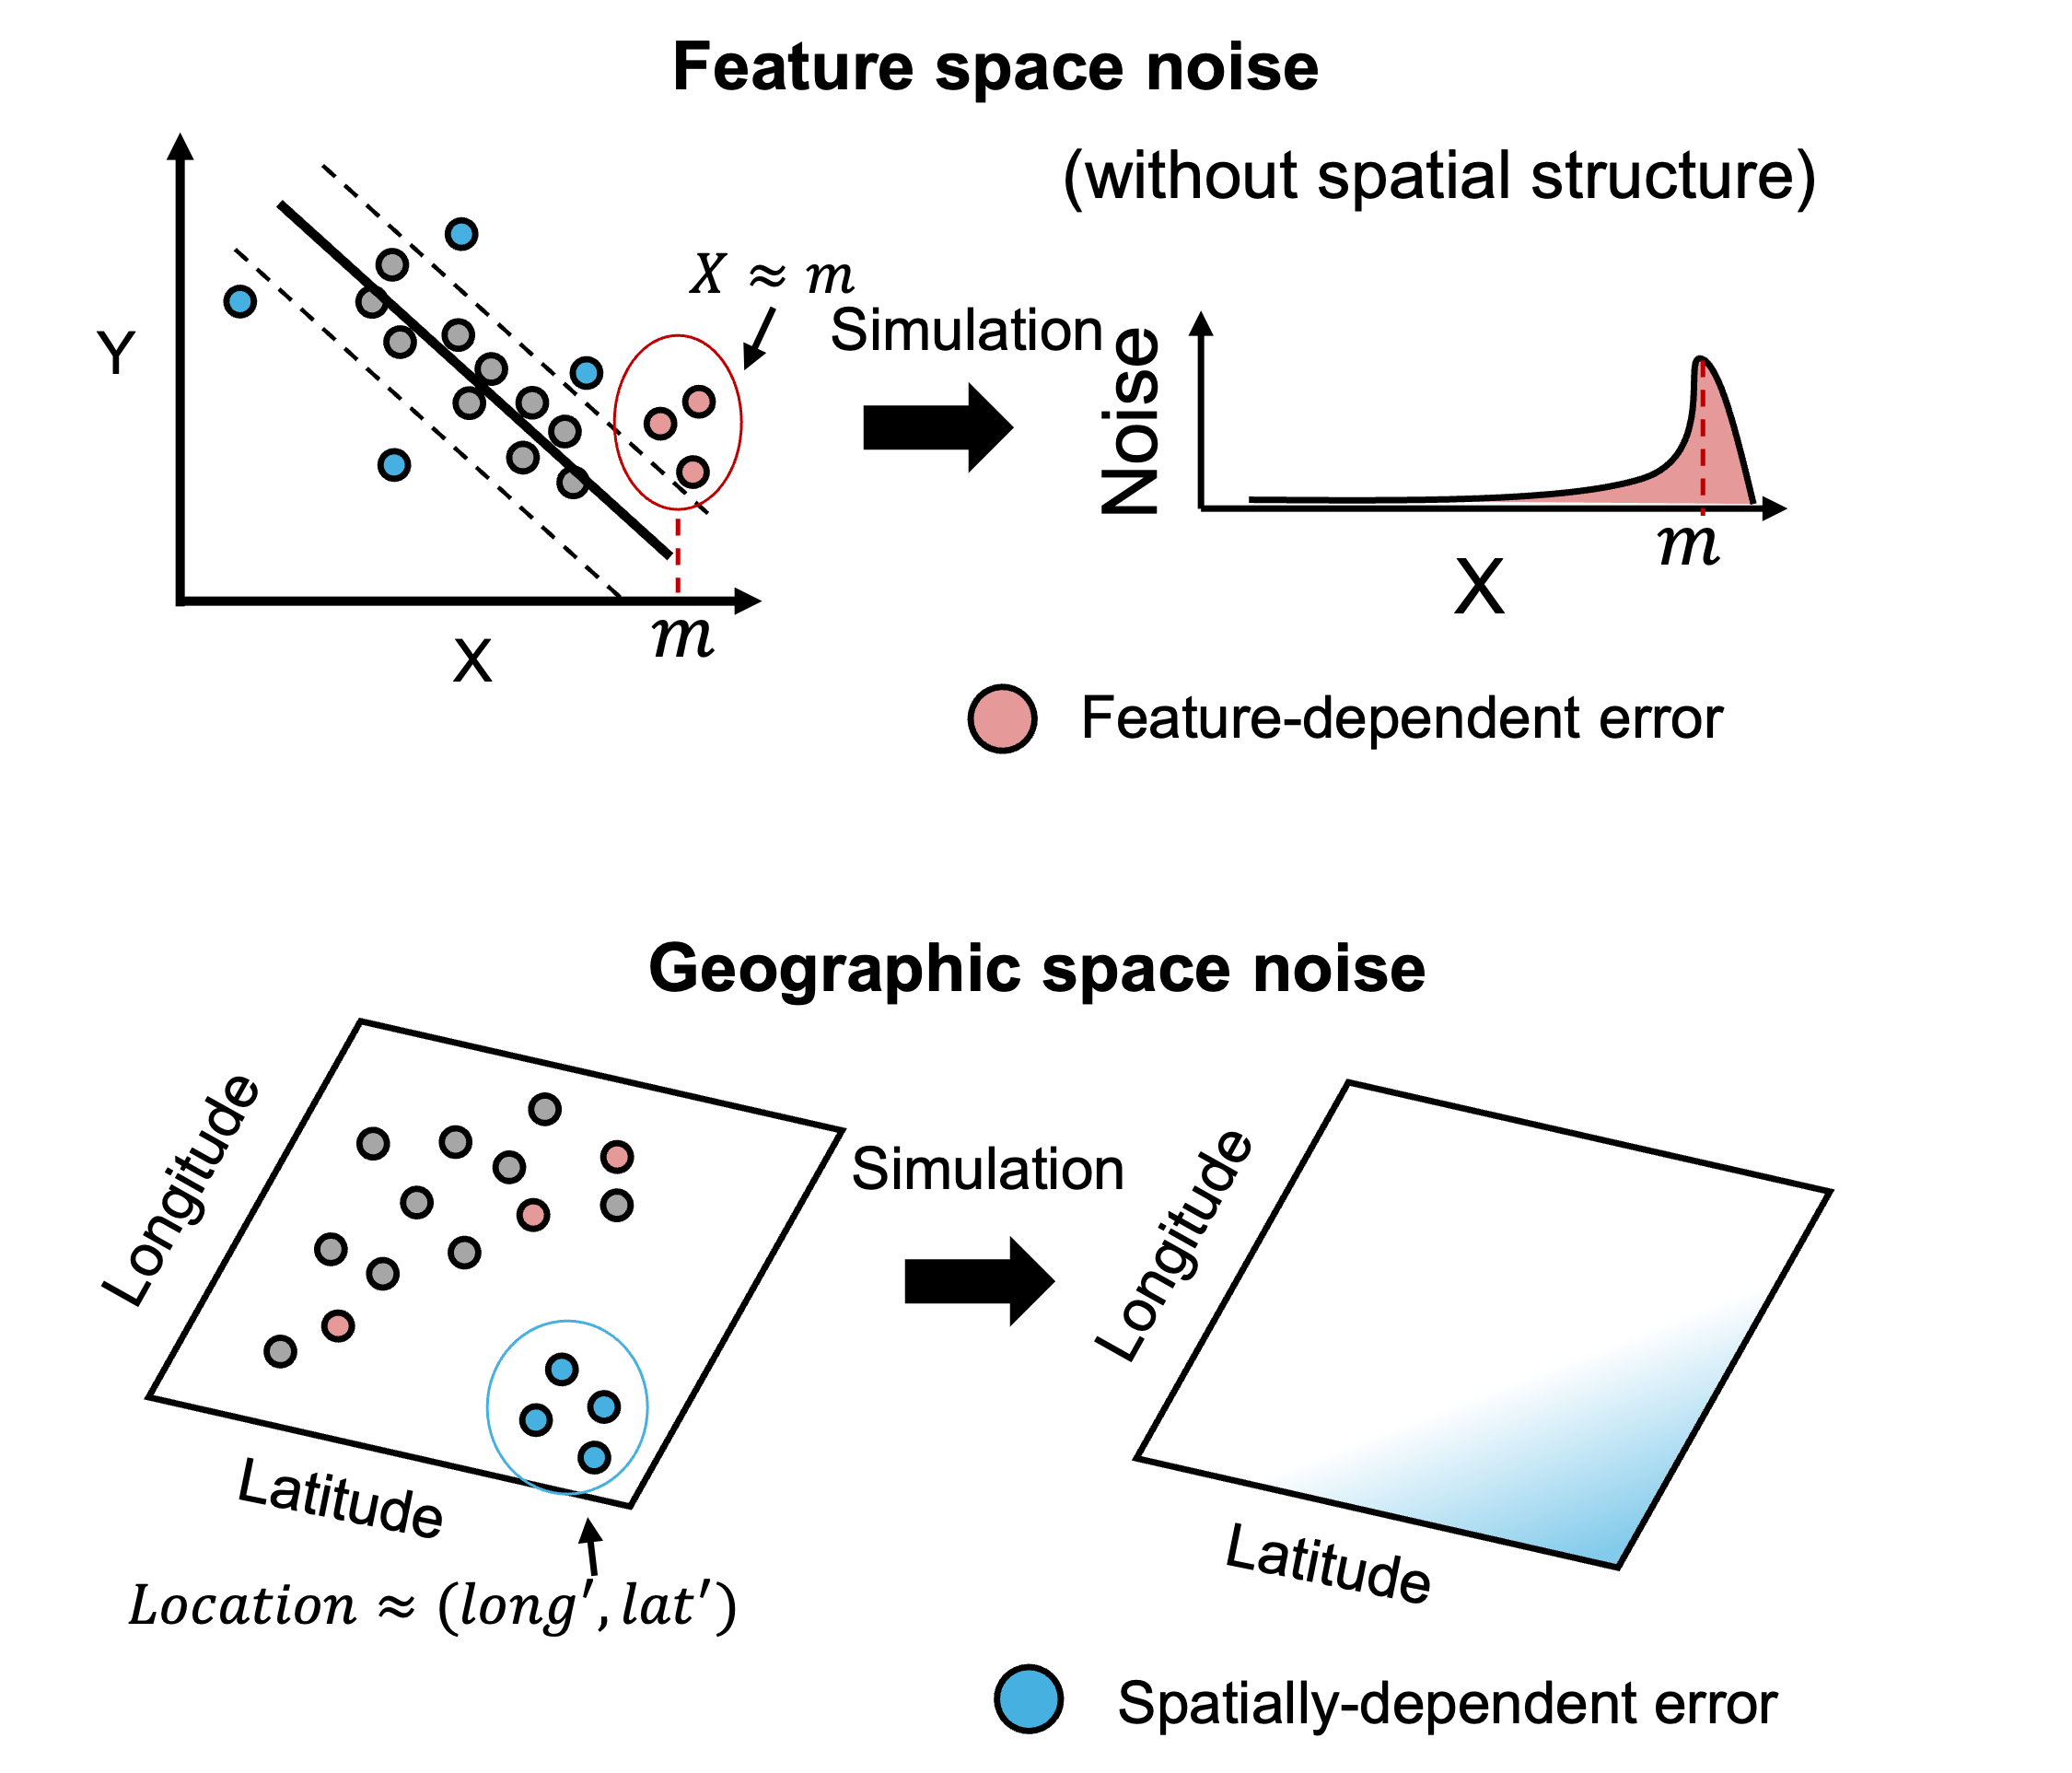
\includegraphics[width=0.8\linewidth]{Figures/FigureX_noise_simulation.png}
    \caption{Simulation of two noise types: Feature space and Geographic space noise}
    \label{fig:simu_noise}
\end{figure*}



Two key parameters govern the structure of both types of noise. First, smoothness Level (\(\sigma_{\text{smooth}}\)) controls the spatial autocorrelation of the noise field, where larger values produce smoother and more spatially coherent uncertainty patterns.  
Second, noise Intensity (\(\sigma_{\text{var}}\)) determines the variance of the noise injected into the target variable, with higher values leading to stronger deviations from the ground truth. This flexible noise generation framework enables controlled experiments under a wide range of spatial and attribute-driven uncertainty conditions, offering a rigorous basis for evaluating the robustness and adaptability of spatial prediction models such as GeoSIMCP.


\subsubsection{Feature space noise}

The feature space noise assumes that uncertainty is not solely a function of space, but is conditioned on the attributes of each observation—i.e., the predictive reliability depends on feature characteristics. This corresponds to epistemic uncertainty in machine learning, where model confidence varies across the feature space.

For each sample with a feature vector \(\mathbf{X} \in \mathbb{R}^d\), we compute its proximity to a predefined cluster center \(\mathbf{c} \in \mathbb{R}^d\) in the feature space. This proximity determines a local noise strength \(\eta(\mathbf{X})\), defined as:

\begin{equation}
\eta(\mathbf{X}) = \exp\left( -\frac{\|\mathbf{X} - \mathbf{c}\|^2}{2\sigma_{\text{cluster}}^2} \right),
\end{equation}

which is then used to modulate a Gaussian noise field before spatial smoothing:

\begin{equation}
\varepsilon_{\text{feat}} = \text{GaussianFilter}\left( \eta(\mathbf{X}) \cdot \mathcal{N}(0, \sigma_{\text{var}}^2),\ \sigma_{\text{smooth}} \right).
\end{equation}


Although the noise is modulated by feature values, it is still anchored on the spatial grid after smoothing. This simulates situations where uncertainty is higher in specific regions of the feature space—e.g., low-sample-density zones, feature-space boundaries, or transitions between regimes. Heterogeneous terrain classification, social indicator estimation where model reliability depends on socioeconomic attributes, or predictive uncertainty in underrepresented feature combinations.


\subsubsection{Geographic space noise}

The geographic space noise assumes that uncertainty is inherently spatial, arising from localized geographic phenomena such as environmental variation, measurement bias, or unobserved spatial processes. The theoretical basis lies in classical spatial statistics, where residual error often exhibits spatial autocorrelation due to omitted spatially structured variables.

We first generate independent Gaussian white noise over the \(100 \times 100\) spatial grid and then apply a Gaussian spatial filter to induce spatial smoothness. Formally, the noise field is defined as:
\begin{equation}
\varepsilon_{\text{geo}} = \text{GaussianFilter}\left( \mathcal{N}(0, \sigma_{\text{var}}^2), \sigma_{\text{smooth}} \right),
\end{equation}
where \(\sigma_{\text{var}}\) controls the overall noise intensity, and \(\sigma_{\text{smooth}}\) determines the degree of spatial autocorrelation.

This setup mimics spatially continuous uncertainty such as sensor error in remote sensing, climate-induced environmental variability, or spatial drift in spatial regression residuals. It is particularly useful for evaluating models’ robustness to geographically correlated noise fields. Environmental modeling, land surface classification, or any setting where error varies smoothly across space (e.g., air quality estimation, land price interpolation).






\subsection{Experimental configurations}

The experiments are conducted on a $100\times100$ spatial grid across a wide range of noise settings. Specifically, we set 9 noise smoothness values and 18 noise intensity values. Two types of noise generation mechanisms are considered: geographic space noise and feature space clustered noise. In totally, 324 datasets with the noise of different spatial process, 162 for each kind os noise.

Specifically, the noise smoothness values ($\sigma_{\text{smooth}}$) are set to: 0.1, 0.5, 1.0, 1.5, 2.0, 2.5, 3.0, 5.0, and 10.0. The noise intensity values ($\sigma_{\text{var}}$) are chosen from a broader range: 0, 0.01, 0.02, 0.03, 0.04, 0.05, 0.06, 0.07, 0.08, 0.09, 0.1, 0.5, 1.0, 2.0, 3.0, 4.0, 5.0, and 10.0. For each noise setting, the bandwidth and trade-off parameter $\lambda$ for GeoSIMCP are tuned separately using a grid search strategy, as detailed in Section~2. Each combination of noise smoothness and intensity is evaluated independently, and all performance metrics are recorded for comparative analysis.


We tested GeoSIMCP model with two different measurements of feature similarity, GeoSIMCP-EUC for the euclidean distance, and GeoSIMCP-MND for the minimum normalized difference. For all simulation experiments, the confidence level of the uncertainty quantification models is set to 90\%.



Although the prediction model is pre-defined and fixed (i.e., a biased predictor with controlled noise) and no model training is required,  
the dataset is initially split into as the normal prediction task: 80\% of the samples are set aside to ensure consistency but are not directly used in model training or evaluation. The remaining 20\% of the data is equally divided into two subsets: 10\% serves as the calibration set for constructing conformal prediction intervals, while the other 10\% is used as the testing set for evaluating model performance in terms of coverage and interval score.

The performance of GeoSIMCP in uncertainty quantification is evaluated using two key metrics: spatial coverage and average interval score (formula 14). Ideally, the predicted uncertainty intervals should achieve high coverage—i.e., contain the true values—with minimal interval width, reflecting both reliability and precision. Given a set of $n$ test samples with true target values $\{y_i\}_{i=1}^n$ and corresponding predicted confidence intervals $[L_i, U_i]$, the spatial coverage $\hat{C}$ is defined as:

\begin{equation}
\hat{C} = \frac{1}{n} \sum_{i=1}^n \mathbb{I}\left\{ L_i \leq y_i \leq U_i \right\}
\end{equation}

where $\mathbb{I}\{\cdot\}$ is the indicator function that equals 1 if the condition holds and 0 otherwise. This metric reflects the proportion of test samples whose true values are successfully captured by their respective prediction intervals.




%Ideally, under a miscoverage level $\alpha$, the target coverage rate is $1 - \alpha$. 
%If $\hat{C} \approx 1 - \alpha$, the prediction intervals are considered well-calibrated.



\subsection{Results}


\subsubsection{Uncertainty quantification under the feature space noise}


% Figure \ref{fig:box_plot_featurenoise} illustrates the distribution of interval scores and coverage for feature space noise under different noise sigma and noise standard deviation. As shown in Figure \ref{fig:box_plot_featurenoise} (a, b), when the noise sigma is small—i.e., when the spatial dependence of the noise is weak—GeoCP exhibits higher interval scores and significantly lower coverage compared to GeoSIMCP. In some cases, such as when sigma = 0.5 or 1.0, the coverage of GeoCP even falls below the target confidence level of 0.9, whereas GeoSIMCP consistently maintains coverage well above 0.9. As noise sigma increases, the performance of GeoCP gradually approaches that of GeoSIMCP.

% In Figure \ref{fig:box_plot_featurenoise} (c, d), all three models show increasing interval scores with larger noise standard deviations, indicating reduced reliability under higher noise variance. However, the coverage remains largely unaffected by the noise standard deviation across all models.

{
\color{red}

Figure \ref{fig:box_plot_featurenoise} (a, b) illustrates the impact of spatial noise dependence ($\sigma_{smooth}$) on prediction performance. When $\sigma_{smooth}$ is small (e.g., $0.1$ to $1.0$), the noise exhibits high spatial frequency and weak dependence, leading to significant spatial non-stationarity. In this case, GeoCP fails to capture local error distributions, resulting in inflated interval scores and coverage dropping below the $0.9$ target. In contrast, GeoSIMCP maintains robust coverage by leveraging feature-space similarity to construct locally-consistent calibration sets.Notably, GeoSIMCP-MND often outperforms the EUC variant in these high-noise-heterity scenarios. This superiority stems from MND's "bottleneck" logic (Eq. \ref{eq:mnd_direct}), which identifies the least similar feature dimension. By being more sensitive to local attribute outliers that EUC might overlook through global averaging, MND ensures that the calibration samples are strictly representative of the test point’s local uncertainty profile. As $\sigma_{smooth}$ increases, the noise becomes more globally uniform, causing the performance of GeoCP to converge toward GeoSIMCP as the advantage of local adaptation diminishes.

In Figure \ref{fig:box_plot_featurenoise} (c, d), all models exhibit a positive correlation between noise standard deviation and interval scores. This trend reflects the intrinsic uncertainty of the data. As the noise variance increases, wider prediction intervals are mathematically necessary to encompass the ground truth. The fact that coverage remains stable across all $\sigma_{var}$ levels demonstrates the strong adaptivity of the GeoSIMCP framework. Specifically, the similarity-based weighting mechanism effectively captures the heteroscedastic nature of the feature-space noise, allowing the model to "scale" its uncertainty estimates without sacrificing reliability. The consistent performance of MND over EUC in the interval score distribution further suggests that focusing on the most deviated feature dimension (MND) provides a more conservative and thus safer bound for uncertainty estimation when the magnitude of noise fluctuates.

\begin{figure*}[htbp]
    \centering
    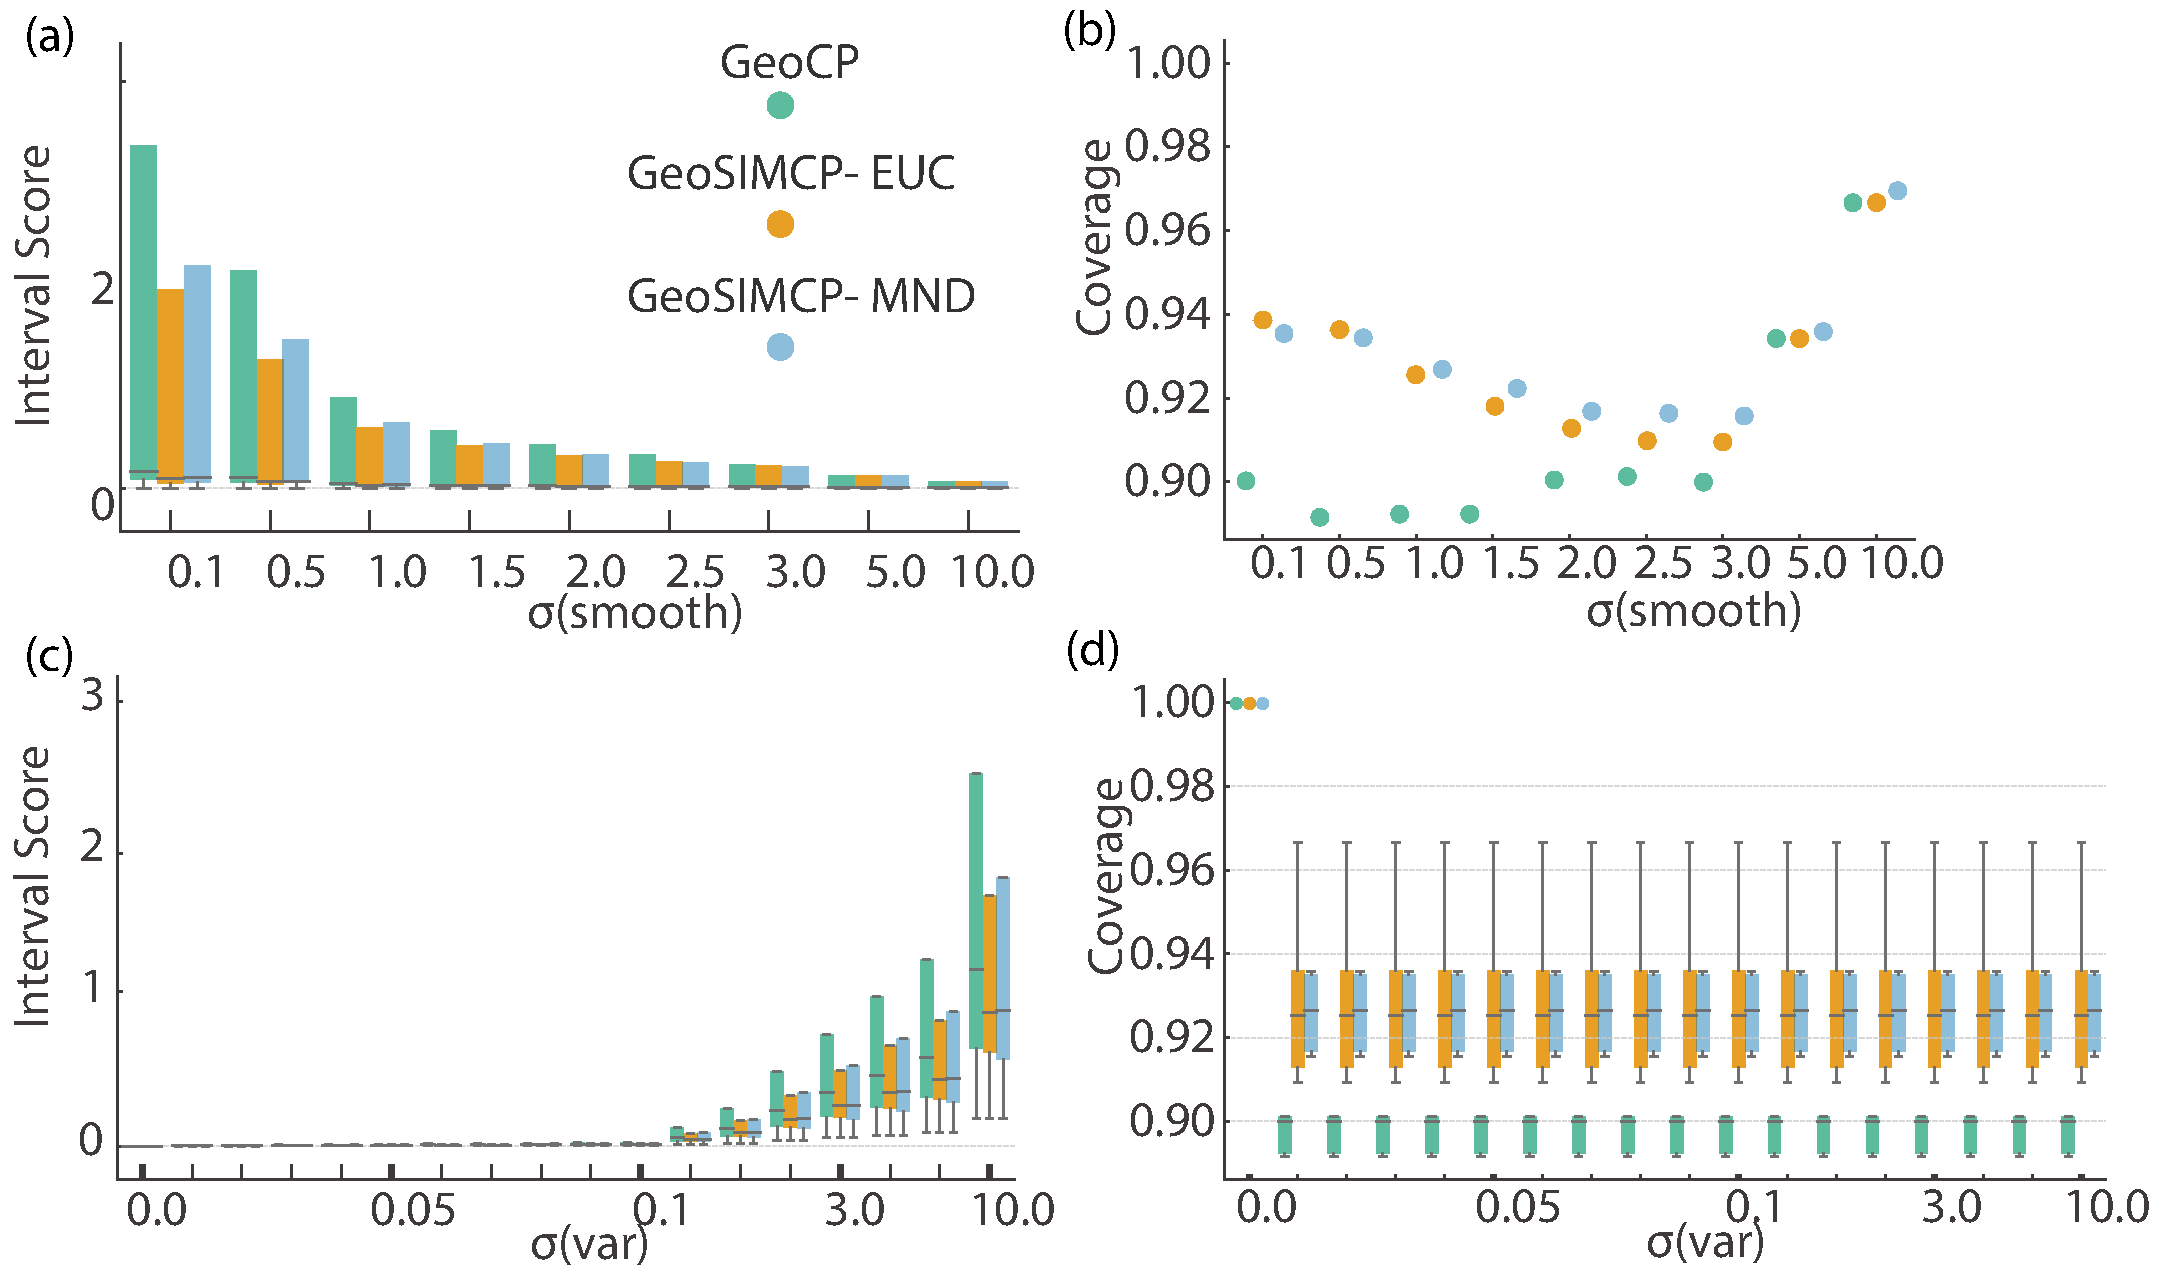
\includegraphics[width=1\linewidth]{Figures/FigureX_simu_interval_score_box.pdf}
    \caption{Distribution of interval scores and coverage under different levels of feature-space noise}
    \label{fig:box_plot_featurenoise}
\end{figure*}

Figure \ref{fig:box_plot_2_featurenoise}a illustrates the estimated uncertainty produced by the three models. Across all noise $\sigma(smooth)$ levels, the predicted uncertainty scales linearly with the noise intensity ($\sigma(var)$). This relationship is consistent with our experimental setup, where the prediction model approximates the "true" data-generating process with controlled simulated noise. The fact that both GeoCP and GeoSIMCP accurately recover this linear scaling law underscores the theoretical validity of the CP framework in quantifying aleatoric uncertainty. As $\sigma(smooth)$ exceeds 3.0, the performance gap among the models narrows significantly. This suggests that as spatial dependence becomes more global, the marginal benefit of feature-space weighting in GeoSIMCP diminishes, leading to converged uncertainty estimates across both global and local CP variants.

Figure \ref{fig:box_plot_2_featurenoise}b reveals the relationship between spatial noise structure and prediction uncertainty. As $\sigma_{smooth}$ increases, the predicted uncertainty for all models decreases. The performance gap narrowing as $\sigma_{smooth}$ exceeds 3.0 further reinforces the theory that GeoSIMCP's primary advantage lies in handling non-stationary, high-frequency spatial noise. When the noise field becomes sufficiently smooth, the distinction between a similarity-weighted local calibration (GeoSIMCP) and a general spatial calibration (GeoCP) diminishes, as the error characteristics at any given point become representative of the broader neighborhood.

% Figure \ref{fig:box_plot_2_featurenoise}b shows that as noise sigma increases, the estimated uncertainty from all three models decreases, while the accuracy improves — reflected by the declining RMSE.


\begin{figure*}[htbp]
    \centering
    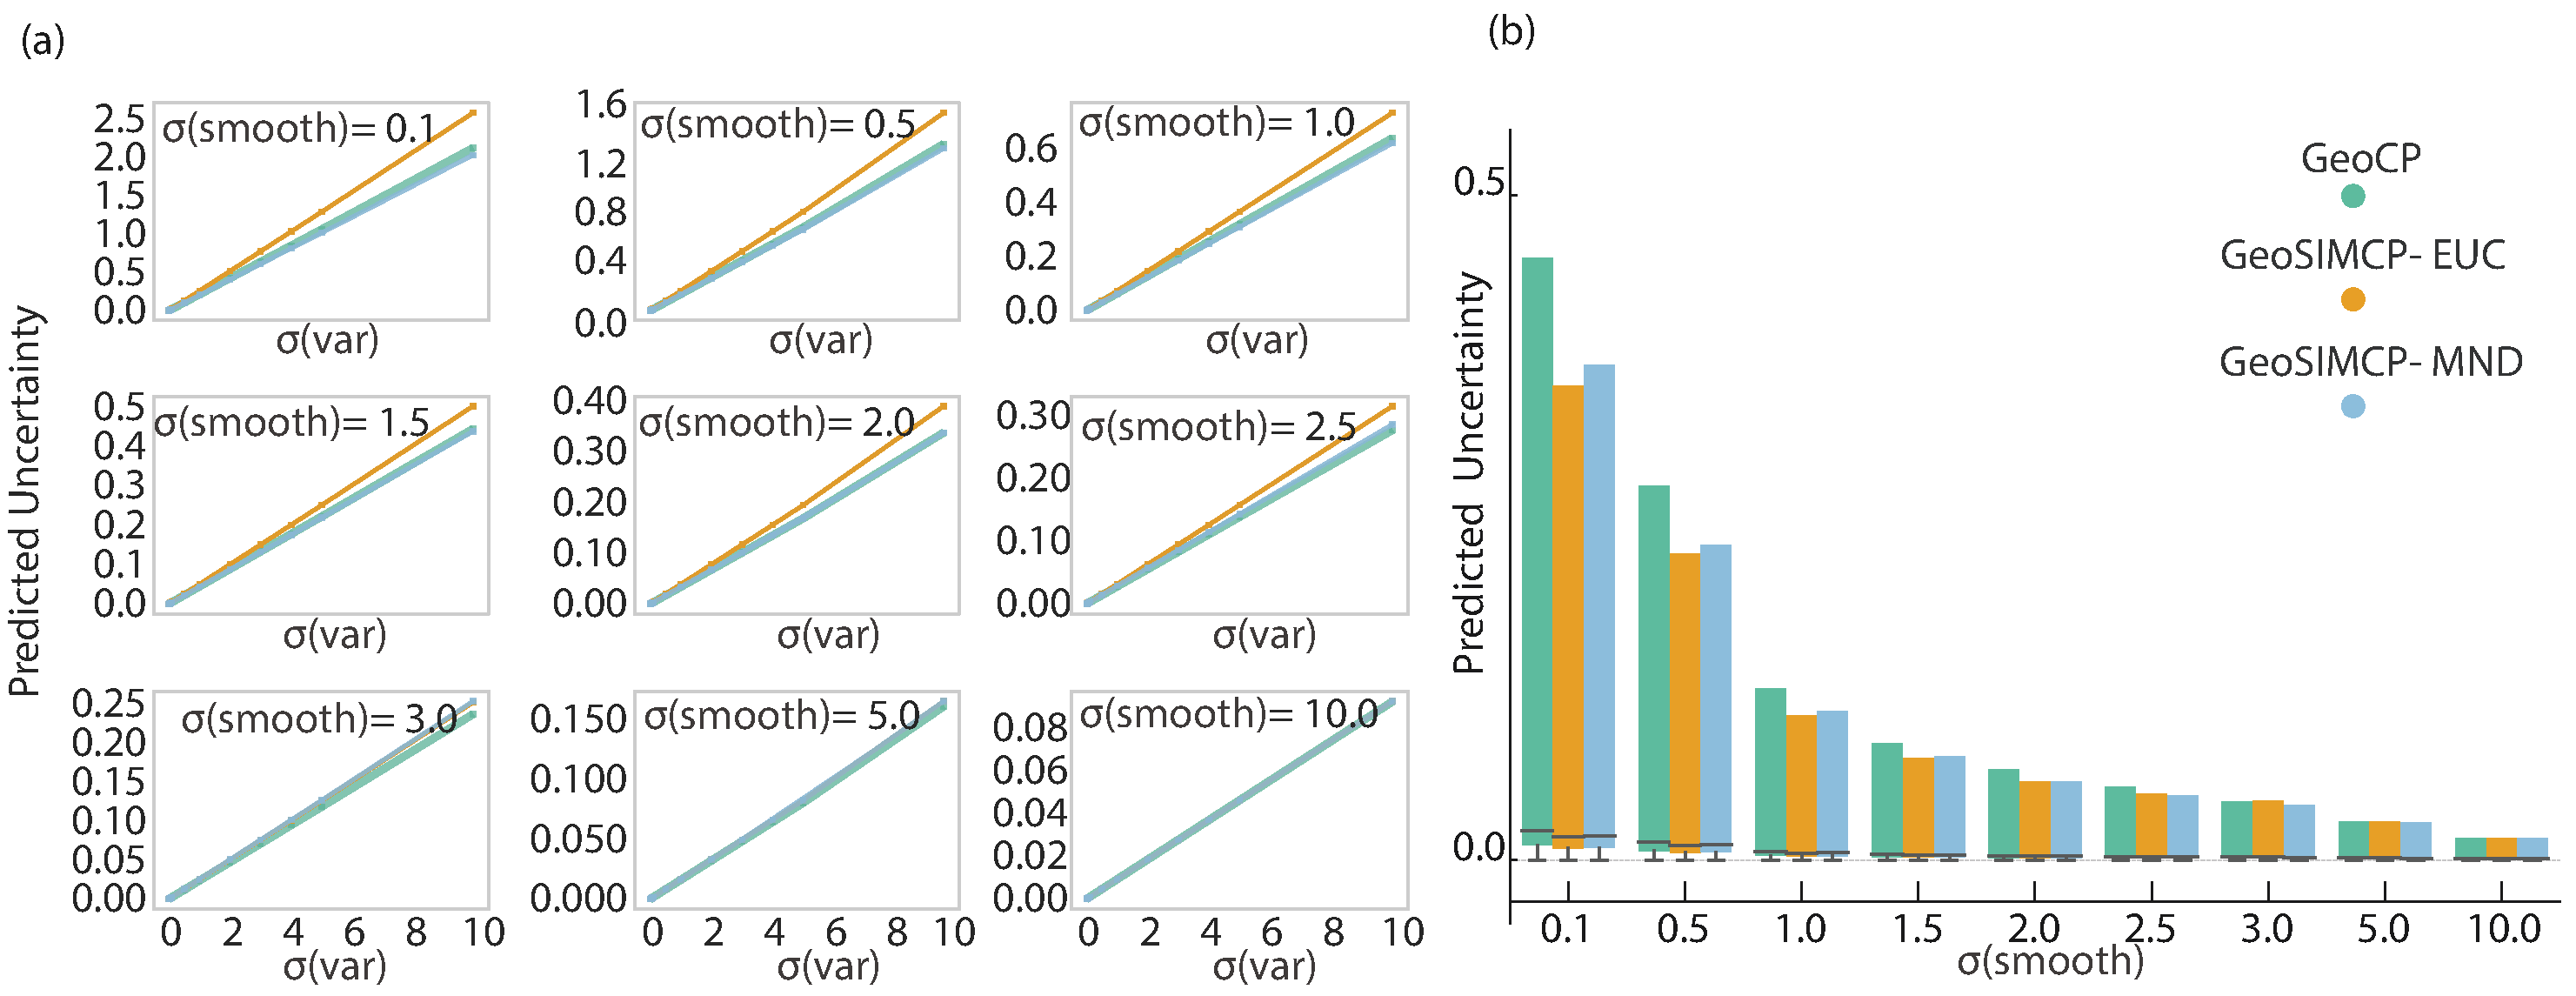
\includegraphics[width=1\linewidth]{Figures/FigureX_simu_uncertainty_rmse_new.pdf}
    \caption{The predicted uncertainty for the feature-space noise experiment from three models: GeoCP, GeoSIMCP-EUC, and GeoSIMCP-MND.}
    \label{fig:box_plot_2_featurenoise}
\end{figure*}



\subsubsection{Uncertainty quantification under the geographical space noise}


This section evaluates the performance of the three models under simulated geographical spatial noise. While noise purely dependent on geographic location is relatively rare in real-world scenarios, this extreme case serves as a stress test to explore the robustness of GeoCP and GeoSIMCP.

Figure~\ref{fig:box_plot_geonoise}a illustrates how the interval scores of the models evolve with varying noise smoothness. When the $\sigma(\text{smooth})$ is set to 0.1, GeoCP achieves the best performance in 11 out of 18 settings. However, as $\sigma(\text{smooth})$ increases, GeoSIMCP consistently outperforms GeoCP. Specifically, when the noise sigma remains below 3, GeoSIMCP achieves the lowest interval scores; once the sigma exceeds 3, GeoSIMCP-EUC becomes the superior model. As shown in Figure~\ref{fig:box_plot_geonoise}b, the coverage of all three models increases alongside the noise sigma. While the models exhibit comparable coverage at low noise sigma values, GeoSIMCP-MND maintains a slight edge in coverage as the sigma increases. Figures~\ref{fig:box_plot_geonoise}c and \ref{fig:box_plot_geonoise}d present the performance of three models across different noise intensities. Overall, GeoSIMCP-MND delivers the best performance, characterized by smaller interval scores and higher coverage.

}


\begin{figure*}[htbp]
    \centering
    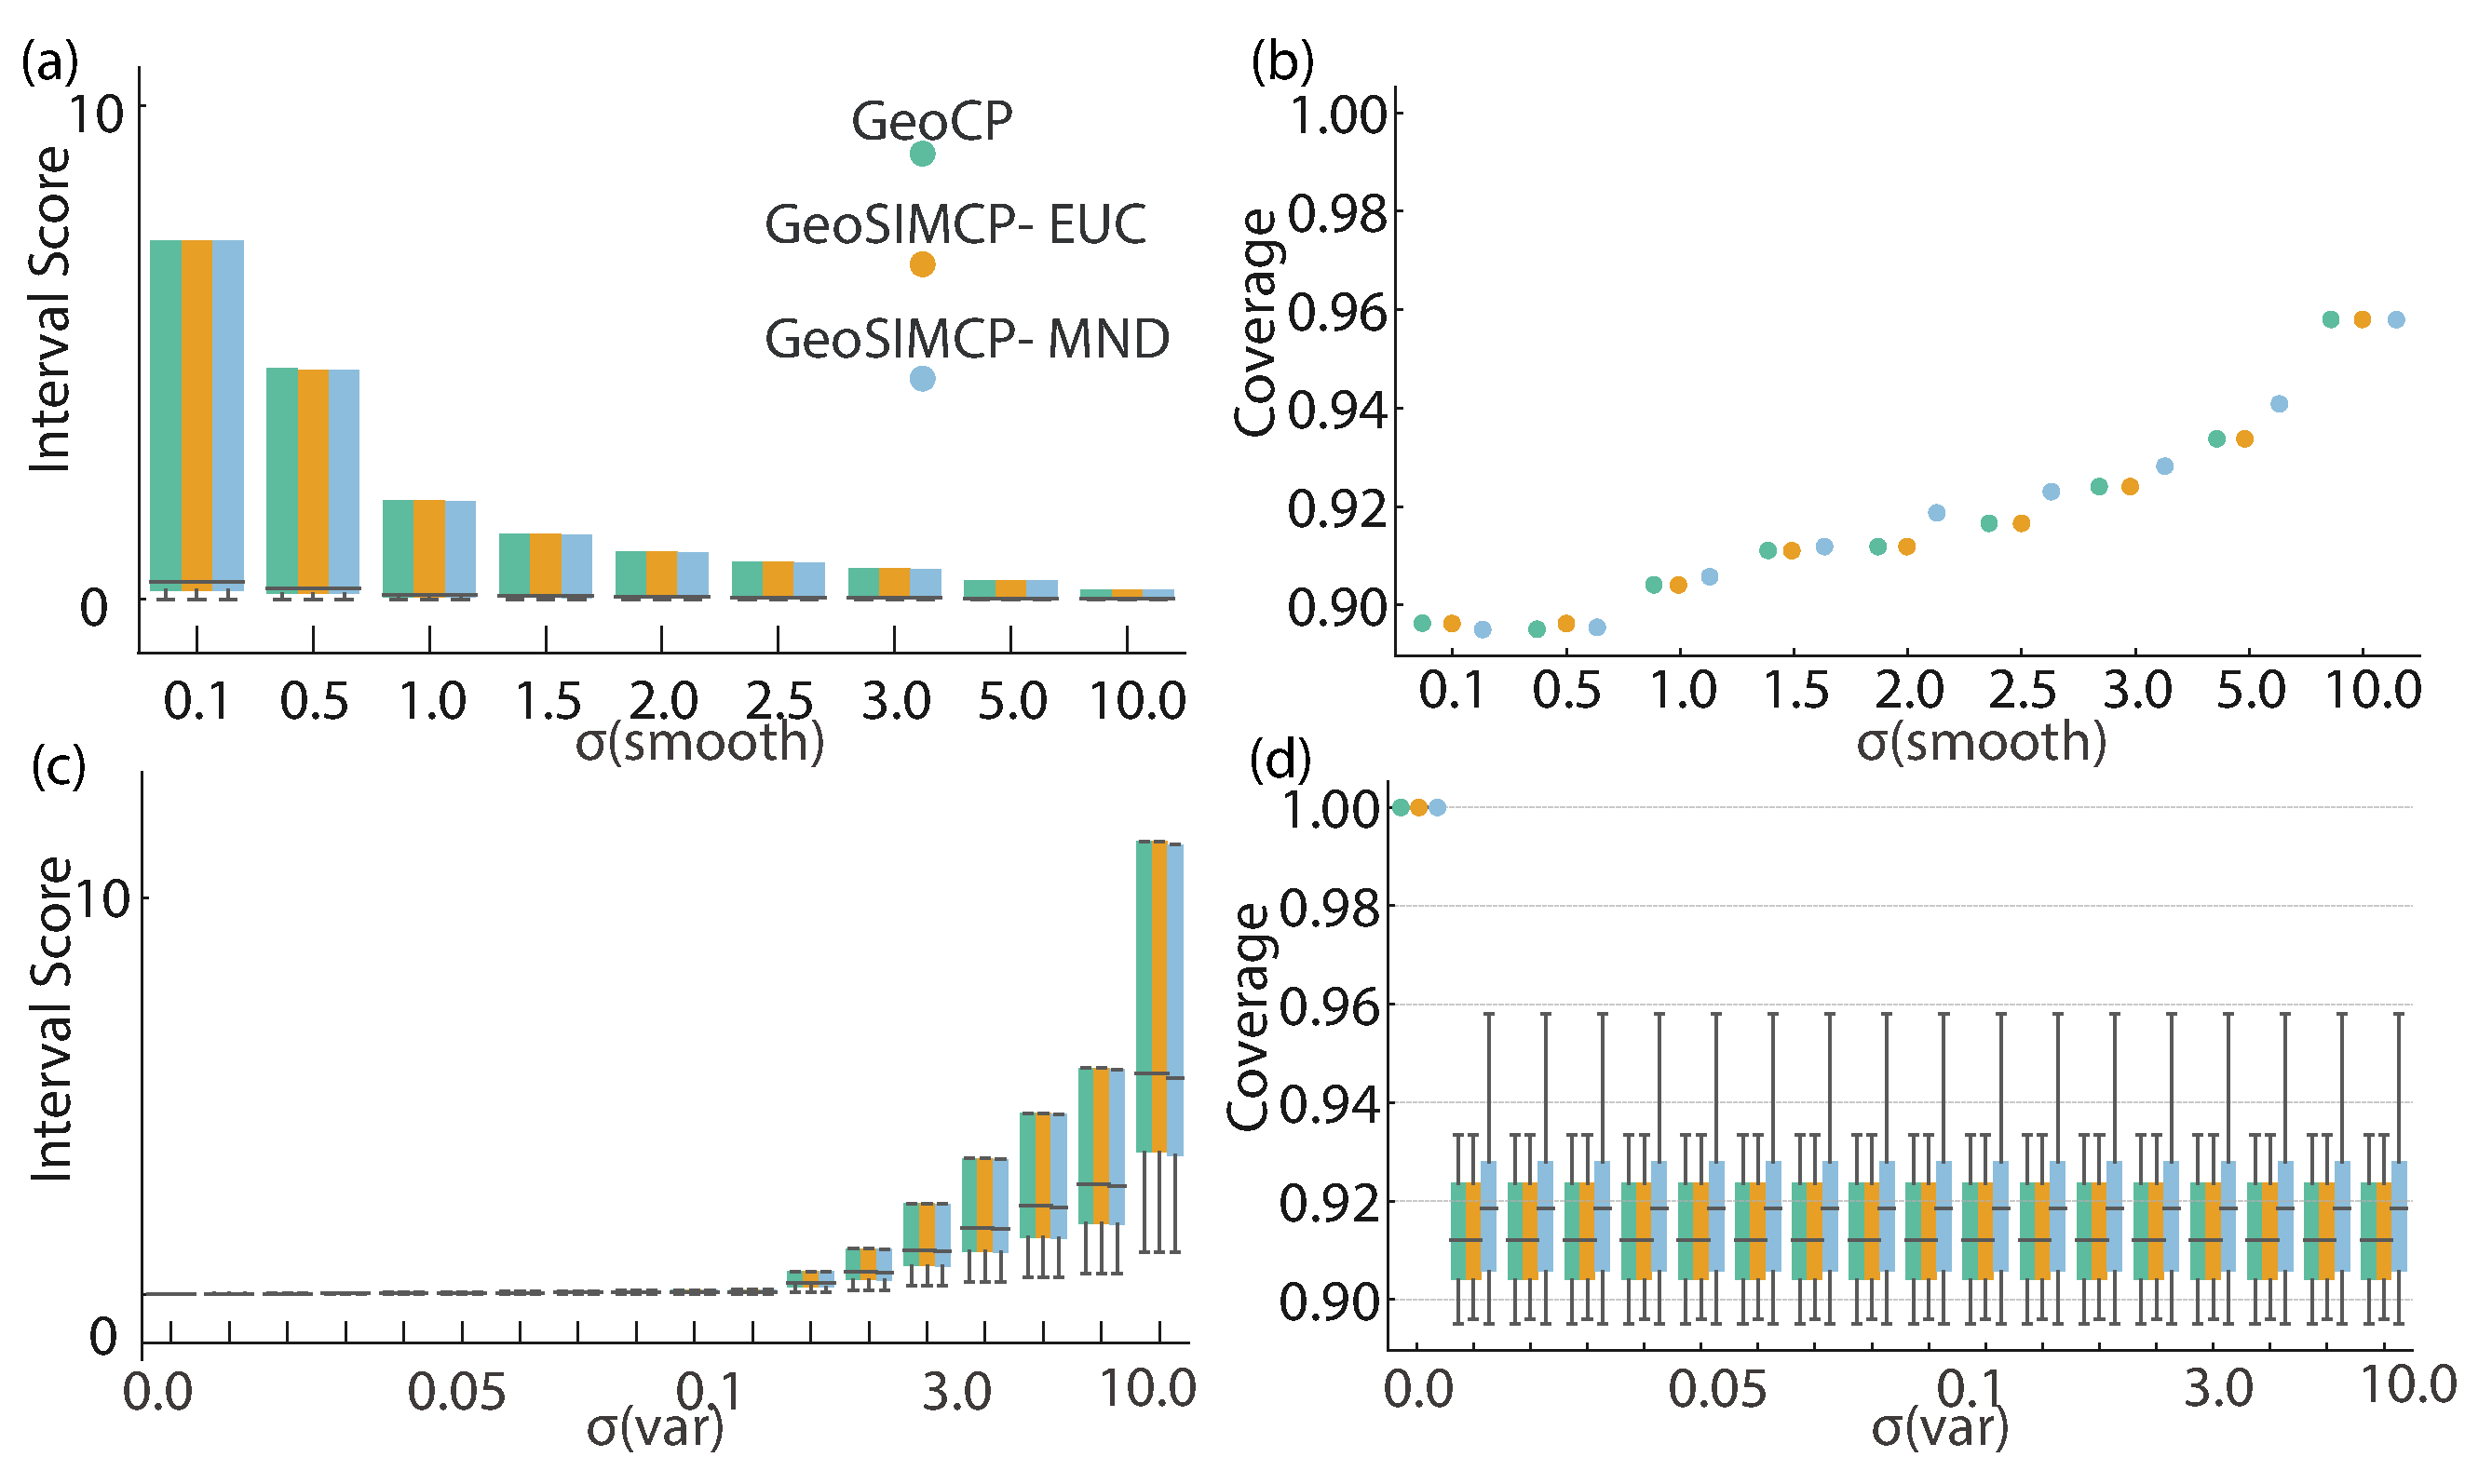
\includegraphics[width=1\linewidth]{Figures/FigureX_simu_interval_score_box_geonoise.pdf}
    \caption{Distribution of interval scores and coverage under different levels of geographical-space noise}
    \label{fig:box_plot_geonoise}
\end{figure*}




\subsubsection{Spatial patterns of uncertainty }

{
\color{red}
As is shown in Figure \ref{fig:uncertainty_mapping}, we visualize the simulated data and the spatial distributions of predictive uncertainty under different noise-generating mechanisms. Three levels of noise smoothness are considered, with $\sigma_{\text{smooth}} = 1, 3,$ and $10$. The left panel shows \emph{feature-space noise}, where perturbations are structured in the attribute space and only weakly aligned with geographic proximity, while the right panel illustrates \emph{geographical-space noise}, where prediction errors are entirely driven by spatial distance.

For feature-space noise, clear differences between GeoCP and GeoSIMCP are observed when $\sigma_{\text{smooth}}$ is small. GeoSIMCP produces uncertainty surfaces that closely follow the underlying noise patterns, successfully capturing localized heterogeneity induced by similarity in the feature space. In contrast, GeoCP, which relies exclusively on geographically weighted conformal calibration, yields overly smooth uncertainty estimates and fails to recover fine-scale variations that are not geographically clustered. This behavior is expected, as GeoCP implicitly assumes that local uncertainty is primarily governed by spatial proximity, an assumption that is violated when noise is organized along attribute dimensions.

As $\sigma_{\text{smooth}}$ increases, feature-space noise becomes progressively smoother and more spatially coherent. Under this regime, the distinction between feature-space similarity and geographic proximity diminishes, and the uncertainty estimates produced by GeoSIMCP and GeoCP converge. This indicates that when noise exhibits strong spatial smoothness, incorporating feature-space similarity provides limited additional benefit beyond geographic weighting alone.

For geographical-space noise, prediction errors are fully determined by spatial proximity. In this setting, GeoSIMCP produces uncertainty patterns that are nearly identical to those of GeoCP across all noise levels. This behavior can be attributed to the adaptive weighting mechanism in GeoSIMCP: the optimized mixing parameter $\lambda$ consistently approaches zero, effectively suppressing the contribution of feature-space distances. Consequently, GeoSIMCP degenerates to GeoCP, and uncertainty estimation is governed exclusively by geographic distance.

It is worth noting that even under purely geographical noise, the uncertainty estimates produced by both GeoCP and GeoSIMCP remain spatially smooth, particularly when $\sigma_{\text{smooth}}$ is small. This is because geographically weighted conformal prediction does not aim to recover point-wise noise realizations, but rather estimates the local scale of the prediction error distribution via kernel-weighted neighborhoods. The combination of distance-based weighting and quantile aggregation acts as a spatial low-pass filter, suppressing high-frequency noise that varies at scales smaller than the kernel bandwidth. As a result, fine-scale geographical noise cannot be resolved unless its spatial smoothness is comparable to the effective neighborhood size. As $\sigma_{\text{smooth}}$ increases and the noise field becomes more spatially coherent, both methods yield more accurate and comparable uncertainty estimates.

Overall, these results demonstrate that the advantage of GeoSIMCP arises specifically in settings where uncertainty is structured by latent feature-space similarity rather than pure spatial proximity, while retaining robustness by adaptively reverting to GeoCP when geographic distance alone explains the error structure.


\begin{figure*}[htbp]
    \centering
    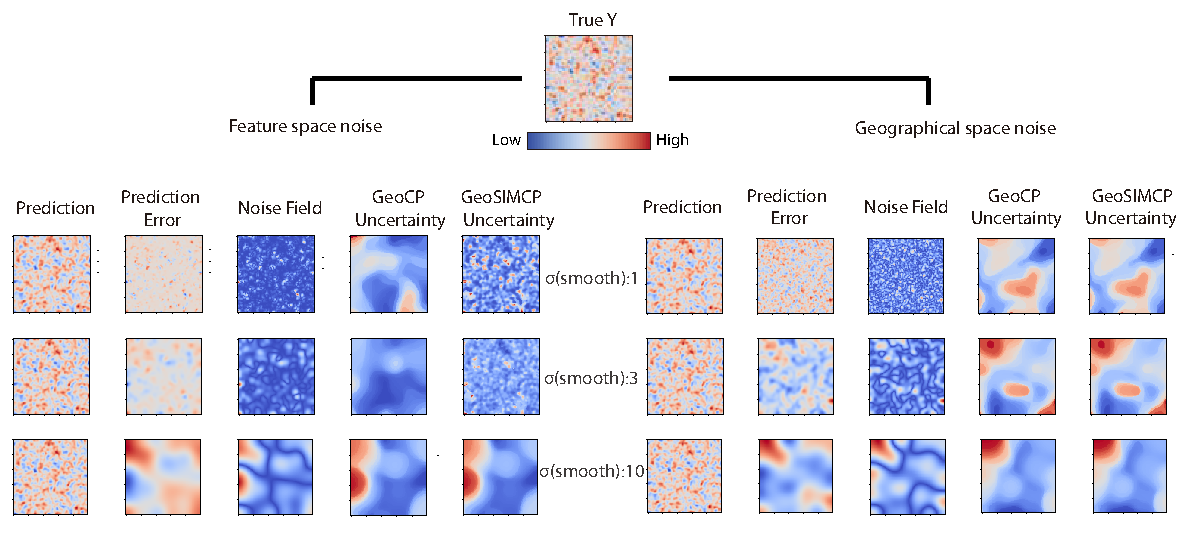
\includegraphics[width=1\linewidth]{Figures/Figure_X_uncertainty_mapping_normal_feature.pdf}
    \caption{Distribution of uncertainty estimated by GeoCP and GeoSIMCP-EUC}
    \label{fig:uncertainty_mapping}
\end{figure*}

}

\section{Real-world experiment}

\subsection{Datasets}


To evaluate the performance of GeoSIMCP in practical settings, we apply it to two real-world spatial prediction tasks: housing price prediction in Seattle and air pollution prediction in China.
 
The Seattle Housing datasets were obtained from the GeoDa Lab repository\footnote{\url{https://geodacenter.github.io/data-and-lab/}}. This dataset includes housing transaction records in Seattle and King County, Washington, between May 2014 and May 2015.Each record provides the sale price along with property characteristics and location. The explanatory variables include \textit{bathrooms}, \textit{sqft\_living}, \textit{sqft\_lot}, \textit{grade}, \textit{condition}, \textit{waterfront}, \textit{view}, \textit{age}, and the coordinates \textit{UTM\_X}, \textit{UTM\_Y}. The full dataset contains 21{,}613 properties; we randomly sample 3{,}000 observations for our experiments to balance spatial coverage and computational efficiency.

% \paragraph{U.S. Life Expectancy.}
% This dataset contains male life expectancy at birth for U.S. counties, with the prediction target being the life expectancy in the first income quartile. The explanatory variables include a set of demographic and diversity indicators: \textit{Diversity Index}, \textit{Asian alone (\%)}, \textit{Native Hawaiian (\%)}, \textit{Two or more races (\%)}, \textit{Hispanic (\%)}, \textit{White alone (\%)}, as well as geographic coordinates (\textit{latitude, longitude}). The dataset covers 3{,}984 counties across the United States.

The China PM\textsubscript{2.5} concentration dataset focuses on PM\textsubscript{2.5} air pollution levels across China for the year 2018. The response variable is the annual mean PM\textsubscript{2.5} concentration, and the predictors include meteorological and remote sensing variables such as \textit{DEM (elevation)}, \textit{surface pressure (sp)}, \textit{temperature (tp)}, \textit{boundary layer height (blh)}, \textit{relative humidity (r)}, \textit{satellite-derived AOD (aod\_sat)}, \textit{vegetation index (ndvi)}, and spatial coordinates (\textit{longitude, latitude}). The dataset includes 1{,}415 monitoring stations distributed across mainland China.





 

\subsection{Experiment design}



\begin{figure*}[htbp]
    \centering
    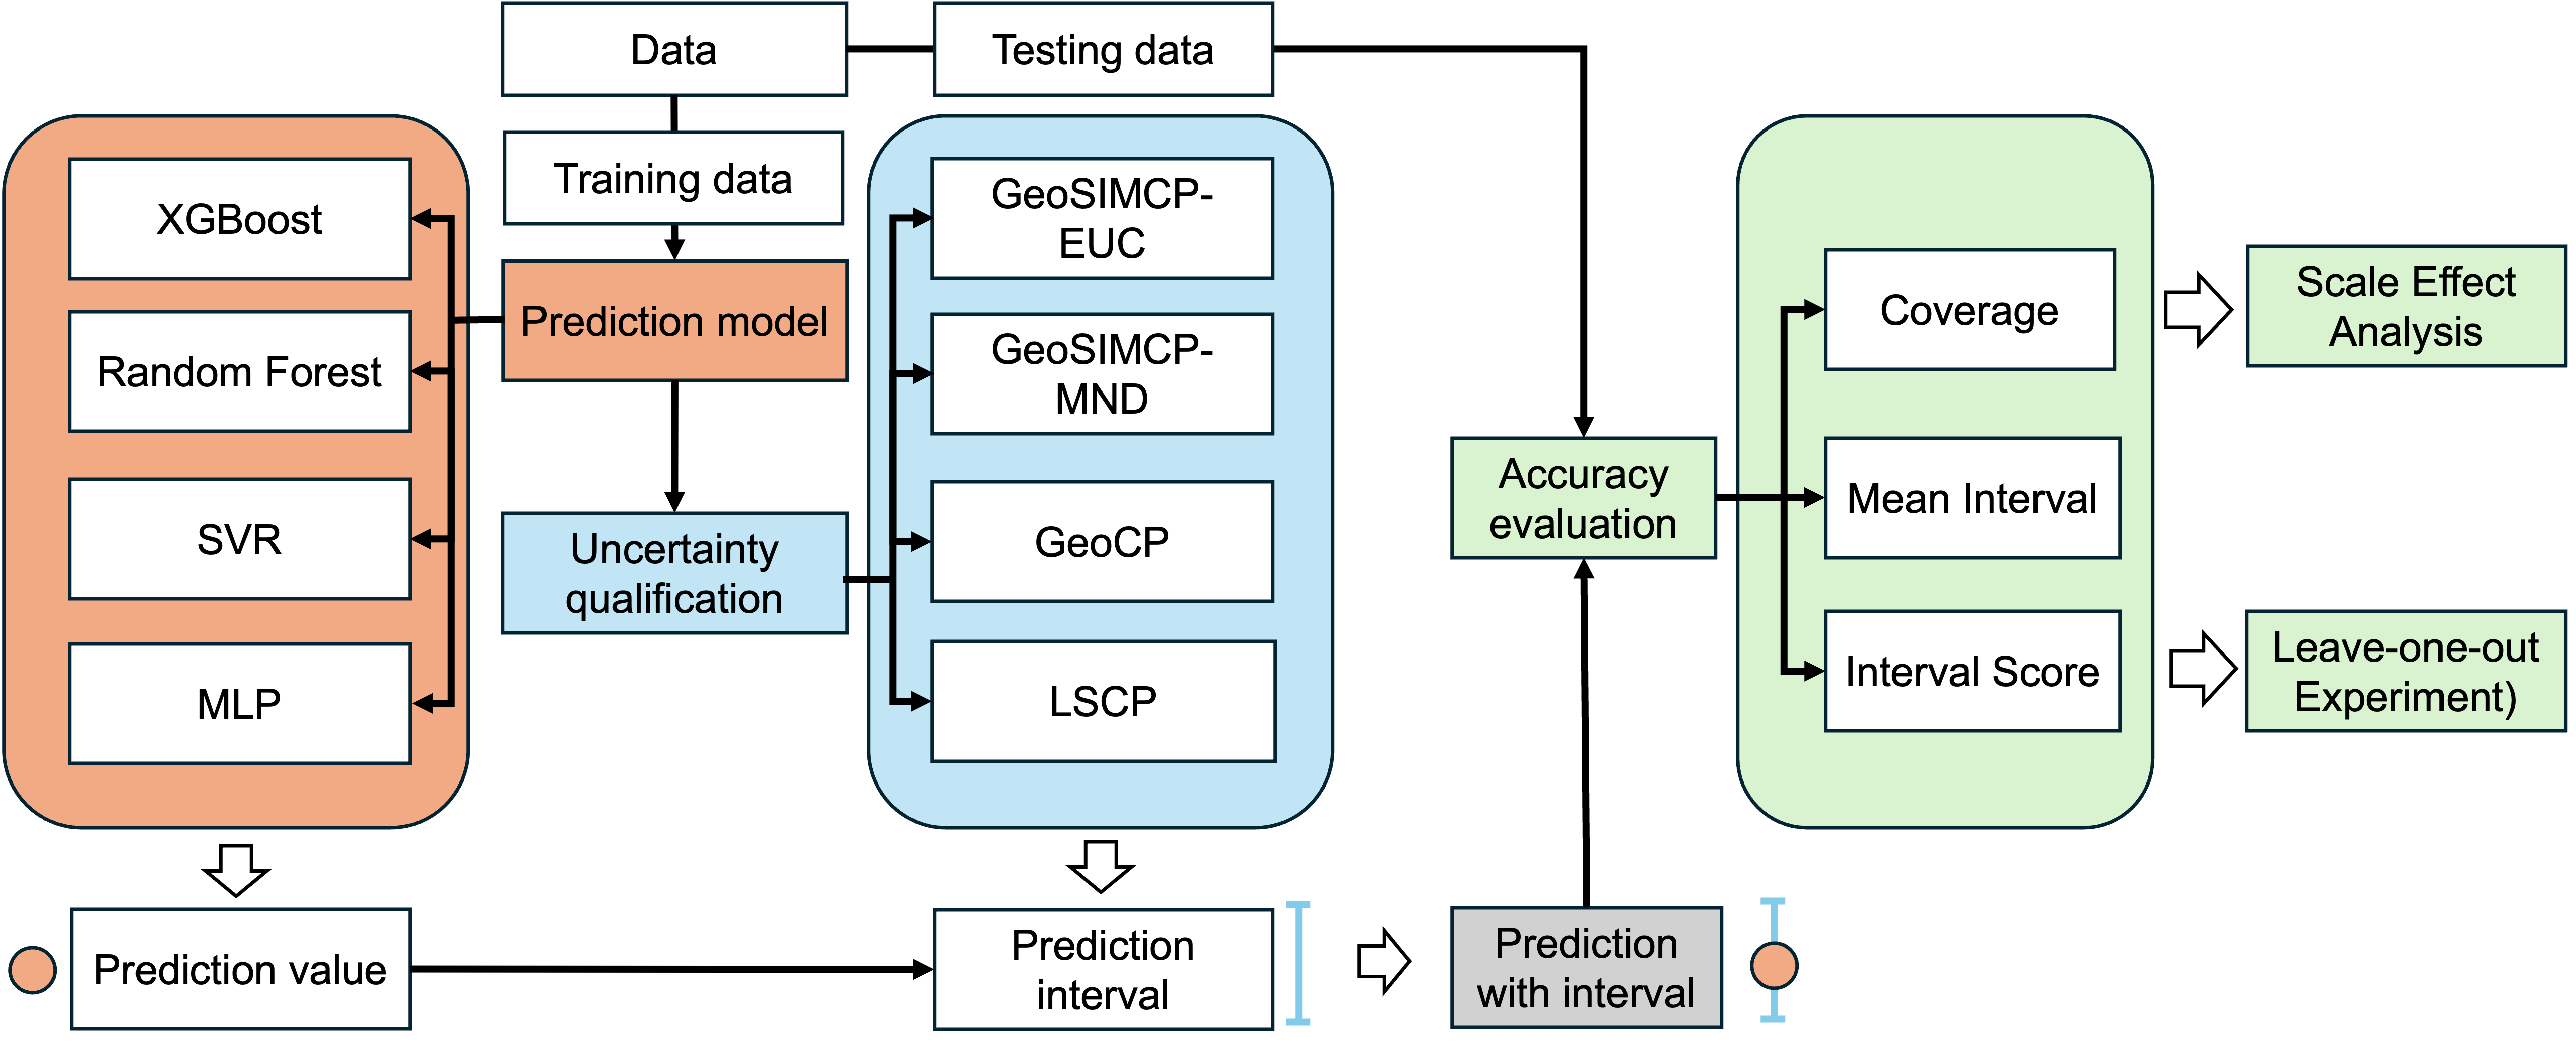
\includegraphics[width=1\linewidth]{Figures/FigureX_true_design_new.png}
    \caption{Experiment design for real world study}
    \label{fig:model_design}
\end{figure*}



\subsubsection{Prediction and uncertainty quantification}
As is shown in Figure \ref{fig:model_design}, we employ four machine learning regression models—XGBoost, Random Forest, Support Vector Regression (SVR), and Multi-Layer Perceptron (MLP)—to perform prediction tasks on three datasets, and apply GeoSIMCP to quantify the associated prediction uncertainty. Each dataset is randomly partitioned into training (80\%), validation (10\%), and testing (10\%) subsets. The models are trained on the training set, with hyperparameter tuning conducted on the validation set. Evaluation of both predictive accuracy and uncertainty quantification is carried out on the testing set.

The XGBoost model is implemented using the \texttt{xgboost} Python package, while the remaining three models are implemented using the \texttt{scikit-learn} library. For each model, we define a corresponding hyperparameter search space and optionally perform grid search for tuning. Specifically, for XGBoost, the hyperparameters include the number of trees (\texttt{n\_estimators}), maximum tree depth (\texttt{max\_depth}), minimum child weight (\texttt{min\_child\_weight}), and column subsampling ratio (\texttt{colsample\_bytree}). For Random Forest, we tune the number of trees and maximum depth. For SVR (\texttt{sklearn.svm.SVR}), we explore the regularization parameter \texttt{C} and the kernel coefficient \texttt{gamma}. For MLP, we vary the hidden layer configuration (\texttt{hidden\_layer\_sizes}) and the L2 regularization strength (\texttt{alpha}), with the maximum number of iterations fixed at 1000. When hyperparameter tuning is enabled, we apply \texttt{GridSearchCV} with 3-fold cross-validation, selecting the model that minimizes the mean squared error. Otherwise, models are used with default parameters and fixed random seeds to ensure reproducibility.

To identify the optimal parameter configuration for GeoSIMCP, we perform a grid search over two key hyperparameters: the kernel bandwidth and the spatial–feature trade-off coefficient. Specifically, the bandwidth $b$ is varied over 20 evenly spaced values in the range $[0.1, 5.0]$, and the trade-off parameter $\lambda$ is searched within the interval $[0, 1]$ with a step size of $0.05$.

We assess the performance of GeoSIMCP in quantifying predictive uncertainty on the testing set. Specifically, we evaluate three standard metrics: interval coverage, average interval width, and the interval score, which together reflect the quality of calibration and the informativeness of the intervals. The confidence level is fixed at 90\% throughout all experiments.


For comparison, we benchmark GeoSIMCP against two baseline methods: LSCP and GeoCP. To ensure a fair comparison, both methods are also tuned via grid search. For LSCP, the number of neighbors $k$ is selected from the discrete set $\{5, 8, 10, 15, 20\}$, while GeoCP is optimized using the same bandwidth search range as GeoSIMCP, that is, $b \in [0.1, 5.0]$ with 20 grid points. For all the uncertainty quantification models, the prediction intervals are constructed at a 90 \% confidence level.

\subsubsection{UQ performance across scale and MAUP}
{
\color{red}

Beyond validating the UQ performance of GeoSIMCP, we also investigated the robustness of its performance across multiple spatial scales and under the Modifiable Areal Unit Problem (MAUP).We developed a comprehensive multi-scale and multi-zoning experimental pipeline. The primary objective is to verify whether the localized joint weighted exchangeability—the core theoretical assumption of our method—remains valid as the spatial units of observation are modified. 

We first conducting a scale effect analysis, where point-based observations were aggregated into regular grids of increasing size. For the national-scale China $PM_{2.5}$ dataset, station data were projected into the China Equidistant Albers projection (EPSG:4776) to ensure physically accurate distance calculations at scales of 0, 50, 100, 200, and 500 km, while the Seattle Housing dataset scales ranged from 0 to 5,000 m. 

Second, a zoning effect analysis was performed to assess sensitivity to boundary definitions by fixing the spatial scale and applying random spatial offsets ($\text{offset}_x, \text{offset}_y$) to the grid boundaries. Spatial aggregation was conducted at fixed scales (100 km for China PM${2.5}$ and 1 km for Seattle Housing), while zoning effects were simulated by randomly shifting grid boundaries. This involved 20 independent trials for each dataset, each utilizing a unique random origin for grid tiling to simulate diverse zoning configurations. In every scenario, target variables ($Y$) and covariates ($X$) were averaged within each grid cell to represent the properties of the newly formed areal units.

A critical feature of our experimental design is the complete recalibration of the entire pipeline for every scale and zoning configuration to ensure that the results are not biased by parameters optimized at the point level. Specifically, at each scale or trial, the base predictive models were retrained using 3-fold cross-validated grid search to ensure that the nonconformity scores reflect the optimal predictive performance specific to each spatial unit. Furthermore, we re-executed a two-dimensional grid search for the kernel bandwidth $b$ and the trade-off parameter $\lambda$ for every experiment.
}

\subsubsection{UQ performance in spatial leave one}
{
\color{red}
In addition to the random train--validation--test splits used in the main experiments, we further investigate model behavior under spatially disjoint hold-out settings, which are commonly adopted to assess robustness under spatial extrapolation. This evaluation complements the random-split experiments by explicitly removing spatial proximity between training and test samples, thereby providing a more stringent test of generalization across space.

For both real-world datasets—the Seattle housing price dataset and the China PM$_{2.5}$ dataset—we construct spatially disjoint train--validation--test splits using geographic clustering. Specifically, spatial locations are partitioned into a fixed number of clusters using $k$-means based solely on spatial coordinates, without incorporating any attribute or response variables. In each split, one cluster is held out entirely as the test region, while the remaining clusters are further divided into training and validation sets, with the validation set used exclusively for uncertainty calibration.

For the Seattle housing price dataset, properties are clustered using projected UTM coordinates to ensure distance-consistent spatial partitioning. In each iteration, one spatial cluster is designated as the test set, while the remaining clusters are randomly split into training (80\%) and validation (20\%) subsets. This procedure is repeated by rotating the held-out cluster, resulting in a region-wise cross-validation scheme that evaluates model performance across distinct urban subregions.

For the China PM$_{2.5}$ dataset, monitoring stations are clustered based on longitude and latitude into multiple geographically coherent regions. In each iteration, all stations within one cluster are completely excluded from both training and validation and are used solely for testing, while the remaining clusters are split into training and validation subsets following the same protocol as above. As a result, regression models are trained exclusively on data outside the test region, ensuring that predictions for the held-out cluster require spatial extrapolation rather than local interpolation.

}
\subsection{Results}


\subsubsection{Accuracy evaluation of spatial prediction}

To evaluate the predictive performance of the XGBoost model on two datasets, we compute standard regression metrics, including root mean square error (RMSE), mean absolute error (MAE), and the coefficient of determination ($R^2$), on both the validation and test sets. As summarized in Table~\ref{tab:model_accuracy_all}, tree-based models consistently outperformed others. Specifically, the Random Forest model achieved the highest performance on the China PM\textsubscript{2.5} dataset ($R^2 = 0.802$), while XGBoost performed best on the Seattle Housing Price dataset ($R^2 = 0.873$).


\begin{table}[ht]
\centering
\caption{Prediction performance of different models on the test sets across two spatial datasets.}
\label{tab:model_accuracy_all}
\begin{tabular}{llccc}
\toprule
\textbf{Dataset} & \textbf{Model} & \textbf{RMSE} & \textbf{MAE} & \textbf{$R^2$} \\
\midrule
\multirow{4}{*}{China PM\textsubscript{2.5}} 
  & XGBoost        & 5.142  & 4.048  & 0.764 \\
  & Random Forest  & 4.711  & 3.648  & 0.802 \\
  & SVR            & 10.191 & 8.477  & 0.074 \\
  & MLP            & 10.024 & 8.250  & 0.104 \\
\midrule
\multirow{4}{*}{Seattle Housing} 
  & XGBoost        & 11.120 & 7.135  & 0.873 \\
  & Random Forest  & 12.769 & 7.350  & 0.833 \\
  & SVR            & 32.100 & 20.822 & -0.057 \\
  & MLP            & 63.502 & 52.723 & -3.137 \\
\bottomrule
\end{tabular}
\end{table}


\subsubsection{Accuracy evaluation of uncertainty quantification}


Table~\ref{tab:pm25} and Table~\ref{tab:housing} presents the uncertainty quantification performance of LSCP, GeoCP, and the two variants of GeoSIMCP across the two real-world datasets. Overall, GeoSIMCP consistently outperforms both LSCP and GeoCP in terms of lower interval score, indicating that it achieves more efficient uncertainty quantification by producing narrower intervals while maintaining the desired coverage.

Specifically, GeoSIMCP-MND (similarity-based) yields the best performance on the housing dataset, while GeoSIMCP-EUC (distance-based) excels on the China PM\textsubscript{2.5} datasets. On the housing dataset, GeoSIMCP-MND reduces the interval score by 33.8\% and 22.4\% compared to LSCP and GeoCP, respectively, highlighting its capacity to produce narrower intervals while maintaining reliability. Similar performance gains are observed across the other datasets.

Among the baselines, GeoCP performs better than LSCP across all datasets, showing its advantage as a spatially adaptive yet model-agnostic method. Moreover, GeoCP exhibits the fastest runtime, completing all predictions in approximately 3 to 5 seconds. In contrast, LSCP incurs the highest computational cost, with runtime reaching up to 51.48 minutes. GeoSIMCP falls between these two extremes: while its runtime is slightly higher than that of GeoCP due to additional feature-based weighting, it remains significantly more efficient than LSCP. In the Appendix, we provide detailed results of hyperparameter optimization for each model. For LSCP, we observe a consistent trend where the coverage improves as the number of neighbors $k$ increases. However, this comes at the cost of wider prediction intervals, as the uncertainty bands expand accordingly.

For GeoCP, the relationship between performance and bandwidth $b$ varies across datasets. In the housing price prediction task, increasing the bandwidth leads to a decline in coverage, suggesting that overly large neighborhoods may smooth out local variability. In contrast, for China PM\textsubscript{2.5} datasets, a larger bandwidth tends to improve coverage, possibly due to more stable underlying spatial structures.
Regarding GeoSIMCP- MND, we find that the optimal values of the trade-off parameter $\lambda$ are $0.737$ for the housing price dataset. This indicates a strong spatial structure in the distribution of uncertainty, where geographic proximity plays an important role in constructing valid intervals.
% Interestingly, for the China PM\textsubscript{2.5} prediction task, both variants of GeoSIMCP (EUC and MND) converge to an optimal $\lambda$ of zero. This suggests that in this case, predictive uncertainty is better captured solely by feature similarity, and geographic proximity does not contribute additional value to uncertainty quantification.

\textcolor{red}{Interestingly, for the China $PM_{2.5}$ prediction task, both variants of GeoSIMCP (EUC and MND) converge to an optimal $\lambda$ of zero. From the perspective of conformal prediction, this indicates that feature-space similarity alone provides sufficient information for defining the local exchangeability of residuals in this context. Rather than suggesting that the spatial process is independent of geography, this result implies that the environmental and meteorological covariates already implicitly encode the underlying spatial structure. Consequently, the joint distance—acting as a heuristic similarity measure to select calibration samples—finds that explicit geographic coordinates offer redundant information for uncertainty quantification. In such cases, feature-space proximity serves as an effective proxy for spatial similarity, leading the optimization of the trade-off parameter $\lambda$ toward the feature domain to achieve the most adaptive calibration.}




\begin{table}[htbp]
\centering
\caption{Uncertainty model performance on China PM$_{2.5}$ dataset}
\label{tab:pm25}
\resizebox{\linewidth}{!}{
\begin{tabular}{lccccccc}
\toprule
UQ Model & Bandwidth & Lambda & $k$ & Coverage & Interval Score & Mean Interval & CPU Time \\
\midrule
\multicolumn{8}{l}{\textit{xgboost}} \\
GeoCP & 2.679 & -- & -- & 0.923 & 23.92 & 10.53 & \textbf{0.35 s} \\
GeoSIMCP-EUC & 2.937 & 0.000 & -- & 0.958 & \textbf{21.99} & 10.18 & 11.32 s \\
GeoSIMCP-MND & 0.358 & 0.000 & -- & 0.944 & 22.20 & 10.11 & 11.71 s \\
LSCP & -- & -- & 20 & 0.901 & 23.26 & \textbf{9.63} & 17.91 min \\
\addlinespace
\multicolumn{8}{l}{\textit{\textbf{random\_forest}} (best prediction performance)} \\
GeoCP & 2.937 & -- & -- & 0.937 & 24.99 & 10.56 & \textbf{1.79 s} \\
GeoSIMCP-EUC & 2.679 & 0.000 & -- & 0.965 & \textbf{21.45} & \textbf{9.64} & 39.36 s \\
GeoSIMCP-MND & 0.616 & 0.000 & -- & 0.958 & 21.75 & 10.11 & 39.86 s \\
LSCP & -- & -- & 20 & 0.901 & 27.32 & 10.96 & 18.14 min \\
\addlinespace
\multicolumn{8}{l}{\textit{svr}} \\
GeoCP & 0.100 & -- & -- & 0.394 & 80.14 & \textbf{7.07} & \textbf{0.54 s} \\
GeoSIMCP-EUC & 1.647 & 0.000 & -- & 0.908 & \textbf{43.28} & 18.96 & 14.01 s \\
GeoSIMCP-MND & 0.100 & 0.000 & -- & 0.873 & 45.05 & 17.20 & 14.25 s \\
LSCP & -- & -- & 5 & 0.768 & 55.12 & 16.38 & 18.41 min \\
\addlinespace
\multicolumn{8}{l}{\textit{mlp}} \\
GeoCP & 3.711 & -- & -- & 0.915 & 45.71 & 19.58 & \textbf{0.32 s} \\
GeoSIMCP-EUC & 2.679 & 0.000 & -- & 0.923 & \textbf{37.58} & 16.37 & 6.69 s \\
GeoSIMCP-MND & 0.358 & 0.000 & -- & 0.908 & 38.11 & \textbf{16.31} & 5.86 s \\
LSCP & -- & -- & 5 & 0.796 & 56.60 & 17.88 & 19.07 min \\
\bottomrule
\end{tabular}
}
\end{table}

\begin{table}[htbp]
\centering
\caption{Uncertainty model performance on Housing Price dataset}
\label{tab:housing}
\resizebox{\linewidth}{!}{
\begin{tabular}{lccccccc}
\toprule
UQ Model & Bandwidth & Lambda & $k$ & Coverage & Interval Score & Mean Interval & CPU Time \\
\midrule
\multicolumn{8}{l}{\textit{\textbf{xgboost}}(best prediction performance)} \\
GeoCP & 0.100 & -- & -- & 0.943 & 54.17 & 19.65 & \textbf{0.60 s} \\
GeoSIMCP-EUC & 1.647 & 0.263 & -- & 0.943 & 47.23 & 17.64 & 17.74 s \\
GeoSIMCP-MND & 0.100 & 0.684 & -- & 0.937 & \textbf{42.01} & 18.03 & 20.77 s \\
LSCP & -- & -- & 5 & 0.797 & 63.44 & \textbf{15.74} & 41.01 min \\
\addlinespace
\multicolumn{8}{l}{\textit{random\_forest}} \\
GeoCP & 0.100 & -- & -- & 0.947 & 59.59 & 21.38 & \textbf{1.14 s} \\
GeoSIMCP-EUC & 0.358 & 0.947 & -- & 0.920 & 48.65 & \textbf{16.80} & 28.53 s \\
GeoSIMCP-MND & 0.100 & 0.737 & -- & 0.923 & \textbf{47.16} & 17.57 & 29.75 s \\
LSCP & -- & -- & 5 & 0.843 & 66.25 & 18.43 & 43.28 min \\
\addlinespace
\multicolumn{8}{l}{\textit{svr}} \\
GeoCP & 0.100 & -- & -- & 0.953 & 148.31 & 58.72 & \textbf{3.48 s} \\
GeoSIMCP-EUC & 1.389 & 0.263 & -- & 0.913 & 104.31 & 37.27 & 52.96 s \\
GeoSIMCP-MND & 0.100 & 0.474 & -- & 0.917 & \textbf{95.88} & 38.66 & 53.66 s \\
LSCP & -- & -- & 5 & 0.850 & 98.21 & \textbf{29.00} & 33.07 min \\
\addlinespace
\multicolumn{8}{l}{\textit{mlp}} \\
GeoCP & 0.100 & -- & -- & 0.927 & 227.66 & 102.98 & \textbf{0.57 s} \\
GeoSIMCP-EUC & 0.100 & 1.000 & -- & 0.927 & 227.66 & 102.98 & 11.38 s \\
GeoSIMCP-MND & 0.100 & 0.842 & -- & 0.910 & \textbf{222.99} & 99.90 & 13.21 s \\
LSCP & -- & -- & 5 & 0.813 & \textbf{219.13} & \textbf{63.29} & 42.33 min \\
\bottomrule
\end{tabular}
}
\end{table}


% \begin{table}[htbp]
% \centering
% \caption{Uncertainty model performance on U.S. Life Expectancy dataset}
% \label{tab:uslife}
% \resizebox{\linewidth}{!}{
% \begin{tabular}{lccccccc}
% \toprule
% UQ Model & Bandwidth & Lambda & $k$ & Coverage & Interval Score & Mean Interval & CPU Time \\
% \midrule
% \multicolumn{8}{l}{\textit{xgboost}} \\
% GeoCP & 1.389 & -- & -- & 0.920 & 103.79 & 40.16 & \textbf{1.91 s} \\
% GeoSIMCP-EUC & 1.389 & 0.947 & -- & 0.922 & 103.06 & 40.22 & 21.53 s \\
% GeoSIMCP-MND & 1.132 & 0.684 & -- & 0.912 & \textbf{102.94} & \textbf{39.86} & 25.27 s \\
% LSCP & -- & -- & 20 & 0.905 & 112.56 & 40.81 & 54.62 min \\
% \addlinespace
% \multicolumn{8}{l}{\textit{\textbf{random\_forest}}(best perdiction performance)} \\
% GeoCP & 1.389 & -- & -- & 0.925 & 97.52 & 39.11 & \textbf{2.66 s} \\
% GeoSIMCP-EUC & 1.389 & 1.000 & -- & 0.925 & 97.52 & 39.11 & 1.06 min \\
% GeoSIMCP-MND & 0.874 & 0.421 & -- & 0.927 & \textbf{96.86} & \textbf{38.83} & 1.10 min \\
% LSCP & -- & -- & 20 & 0.920 & 103.94 & 41.13 & 55.73 min \\
% \addlinespace
% \multicolumn{8}{l}{\textit{svr}} \\
% GeoCP & 5.000 & -- & -- & 0.902 & 121.53 & 53.88 & \textbf{2.99 s} \\
% GeoSIMCP-EUC & 1.905 & 0.105 & -- & 0.902 & \textbf{119.85} & 53.26 & 1.21 min \\
% GeoSIMCP-MND & 3.711 & 0.579 & -- & 0.902 & 121.32 & 53.80 & 1.27 min \\
% LSCP & -- & -- & 5 & 0.792 & 135.08 & \textbf{37.68} & 52.83 min \\
% \addlinespace
% \multicolumn{8}{l}{\textit{mlp}} \\
% GeoCP & 2.937 & -- & -- & 0.902 & \textbf{101.49} & 43.39 & \textbf{0.75 s} \\
% GeoSIMCP-EUC & 2.937 & 1.000 & -- & 0.902 & \textbf{101.49 }& 43.39 & 27.11 s \\
% GeoSIMCP-MND & 2.937 & 1.000 & -- & 0.902 & \textbf{101.49} & 43.39 & 29.40 s \\
% LSCP & -- & -- & 5 & 0.820 & 116.02 & \textbf{36.48} & 55.34 min \\
% \bottomrule
% \end{tabular}
% }
% \end{table}




%\subsubsection{Uncertainty distribution}

We illustrated the prediction outcomes and uncertainty quantification results on the test datasets for two real-world case studies. Specifically, a Random Forest model was implemented for China PM2.5 concentration estimation, while an XGBoost model was utilized for the Seattle housing price prediction task. \textcolor{red}{Figure~\ref{fig:mapping_china} presents the results of the PM${2.5}$ prediction task. Overall, the pointwise relationship between predicted PM${2.5}$ concentrations and associated uncertainty is weak, with an $R^{2}$ of 0.043, indicating that predictive uncertainty is not simply driven by concentration magnitude. The spatial distribution reveals a clear east–west gradient, with PM${2.5}$ concentrations generally decreasing from the eastern coastal regions toward the western inland areas of China. }

\textcolor{red}{Notably, although PM${2.5}$ concentrations are relatively high in North China (e.g., Shandong and Hebei provinces), the corresponding predictive uncertainty remains comparatively low. This suggests that PM${2.5}$ dynamics in this region are more spatially homogeneous and locally predictable, allowing the model to produce stable and reliable predictions. In contrast, the eastern coastal region (e.g., Jiangsu and Zhejiang provinces) exhibits comparable PM${2.5}$ concentration levels but substantially higher predictive uncertainty. This discrepancy indicates that PM${2.5}$ aggregation in coastal regions is governed by more complex and heterogeneous spatial processes, likely involving diverse emission sources, which reduce local predictability and challenge the localized exchangeability assumptions underlying uncertainty calibration.
In Inner Mongolia and other inland regions such as Xinjiang and Tibet, PM${2.5}$ concentrations are generally low; however, predictive uncertainty often exceeds 9.76. This reflects limited data support and weak spatial regularity in these sparsely sampled regions, where PM${2.5}$ generation mechanisms are less constrained by local observations. Consequently, predictions in these areas should be interpreted with caution, as the uncertainty estimates signal reduced local predictability of the underlying spatial process.}


\textcolor{red}{Figure~\ref{fig:mapping_house} presents the results of the housing price prediction task in Seattle.
Unlike the PM$_{2.5}$ case, the scatter plot reveals a clear positive relationship between predicted housing prices and associated uncertainty, indicating that higher-priced properties tend to be accompanied by greater predictive uncertainty. This pattern suggests that uncertainty is not random, but systematically linked to variations in the underlying housing market structure. Alternatively, this indicates that the underlying spatial patterns of Seattle house prices remain inadequately captured by the chosen features and model, thereby leading to significant spatial autocorrelation in the resulting uncertainty.
Spatially, the southern region of Seattle is characterized by relatively lower housing prices and consistently low predictive uncertainty. This indicates that housing prices in these areas are governed by more homogeneous and stable local processes, allowing the model to generate reliable and well-calibrated predictions. In contrast, the northern part of the city—particularly the northeastern neighborhoods—exhibits substantially higher uncertainty, even for properties with comparable price levels. This suggests that the underlying drivers of housing prices in north of Seattle are significantly more complex, involving latent factors that the current model fails to adequately capture.}

% \begin{figure*}[htbp]
%     \centering
%     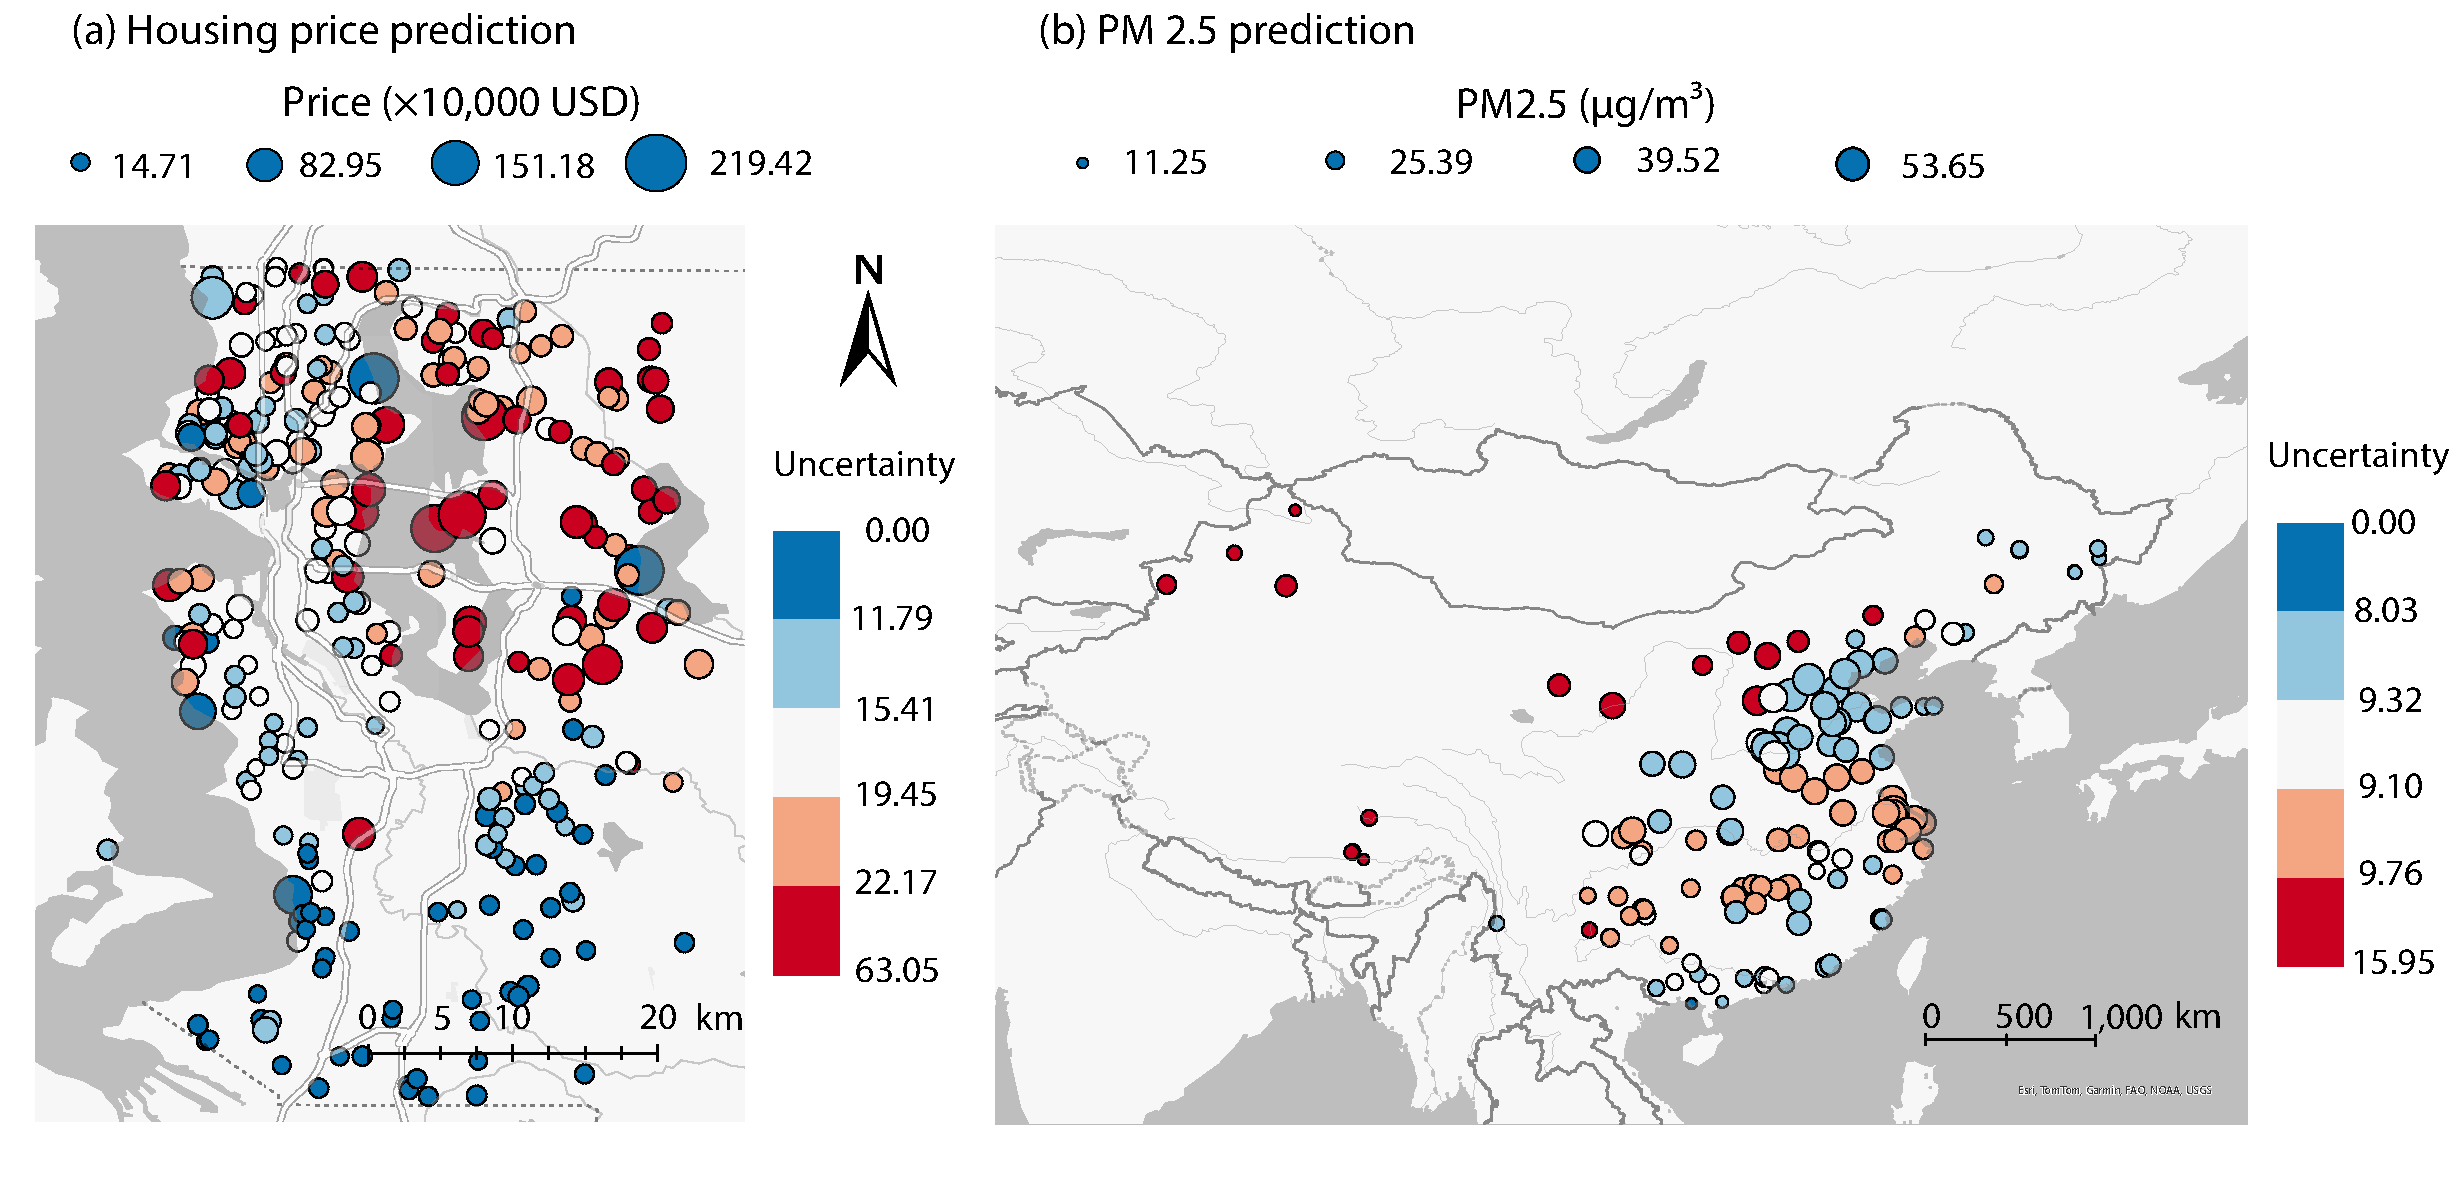
\includegraphics[width=1\linewidth]{Figures/Figure_X_mapping.pdf}
%     \caption{Spatial prediction results from the best-performing machine learning model and uncertainty quantification results from GeoSIMCP for (a) PM2.5 concentrations and (b) housing prices. The predicted value is indicated by the size of each dot, while the color represents the level of uncertainty.}
%     \label{fig:mapping}
% \end{figure*}




\begin{figure*}[htbp]
    \centering
    \includegraphics[width=1\linewidth]{Figures/FigureX_Result_China_new2.pdf}
    \caption{Prediction and uncertainty quantification results for PM2.5 concentrations. The dot size indicates the predicted value from the best-performing machine learning model, while the color encodes the level of uncertainty estimated by GeoSIMCP.}
    \label{fig:mapping_china}
\end{figure*}


\begin{figure*}[htbp]
    \centering
    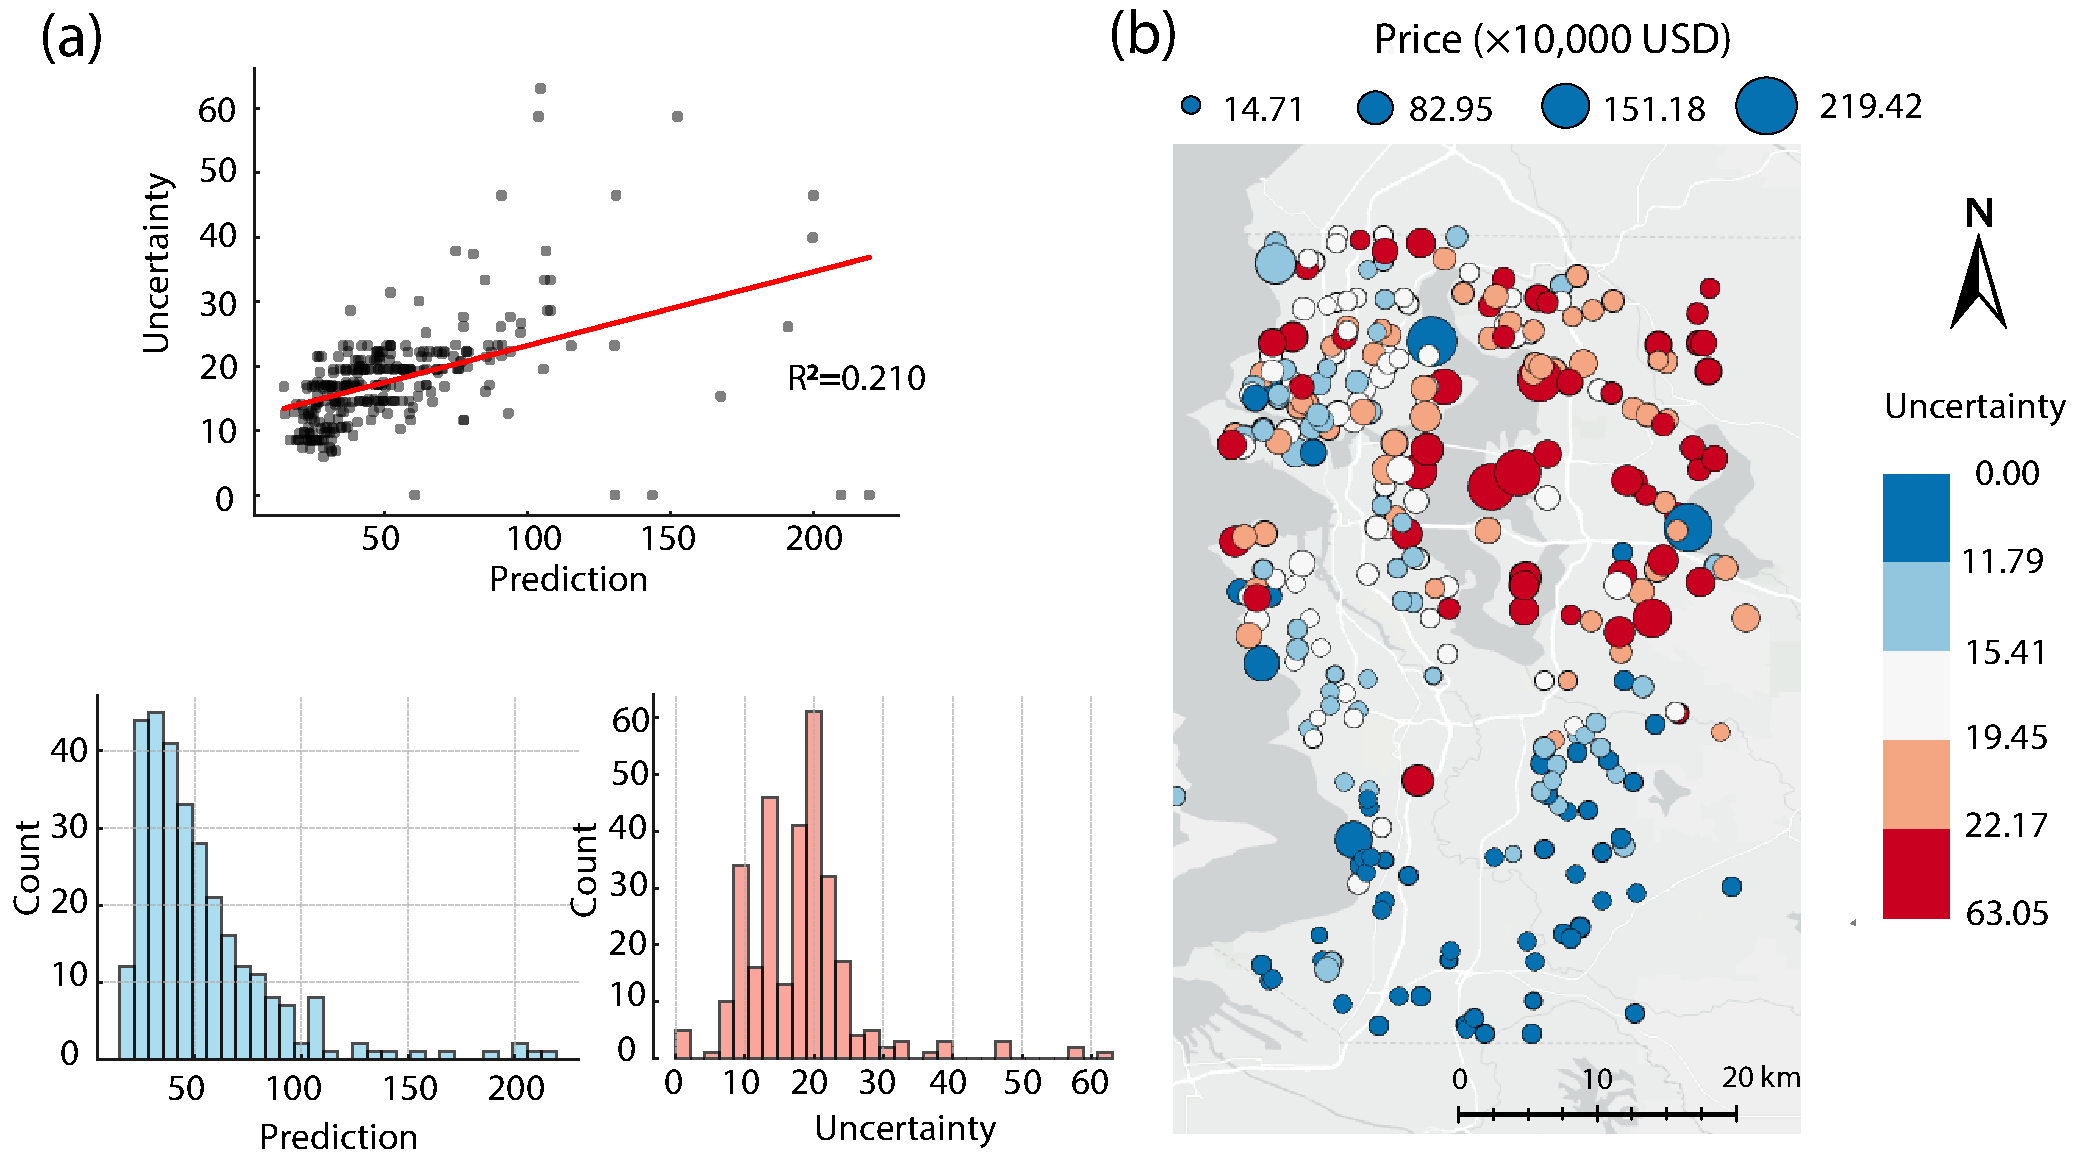
\includegraphics[width=1\linewidth]{Figures/FigureX_Result_housing_new.pdf}
    \caption{Prediction and uncertainty quantification results for housing price. The dot size indicates the predicted value from the best-performing machine learning model, while the color encodes the level of uncertainty estimated by GeoSIMCP.}
    \label{fig:mapping_house}
\end{figure*}



\subsubsection{Performance across different scales}

{
\color{red}


Figure \ref{fig:scale_1} (a,c) illustrates how spatial aggregation affects both the effective sample size and the predictive performance of the base models across increasing spatial scales for the China PM$_{2.5}$ and Seattle Housing datasets. As expected, spatial aggregation leads to a substantial reduction in sample size as the grid resolution becomes coarser. This effect is particularly pronounced for the China PM$_{2.5}$ dataset, where aggregation from point-level observations to grids of 500\,km results in a drastic decrease in the number of spatial units. A similar but more gradual decline is observed for the Seattle Housing dataset due to its higher initial spatial density and smaller aggregation scales.

Figure \ref{fig:scale_1} (b,d)  report the corresponding prediction errors measured by RMSE for the base models at each spatial scale. For both datasets, predictive performance does not change monotonically with spatial aggregation. At fine to intermediate scales, RMSE initially increases, reflecting the combined effects of reduced sample size. As spatial scale continues to increase, RMSE stabilizes or even decreases, particularly at the coarsest resolutions. This behavior suggests that spatial aggregation introduces a trade-off between information loss and noise reduction: while fine-scale aggregation reduces sample support and may obscure local patterns, coarse-scale aggregation smooths high-frequency variability and yields more stable average signals. Importantly, these results confirm that spatial aggregation fundamentally alters both the statistical properties of the data and the achievable predictive accuracy of the underlying models. This motivates the necessity of fully recalibrating uncertainty quantification procedures at each spatial scale, as uncertainty estimates cannot be assumed to transfer directly from point-level observations to aggregated areal units.

\begin{figure*}[htbp]
    \centering
    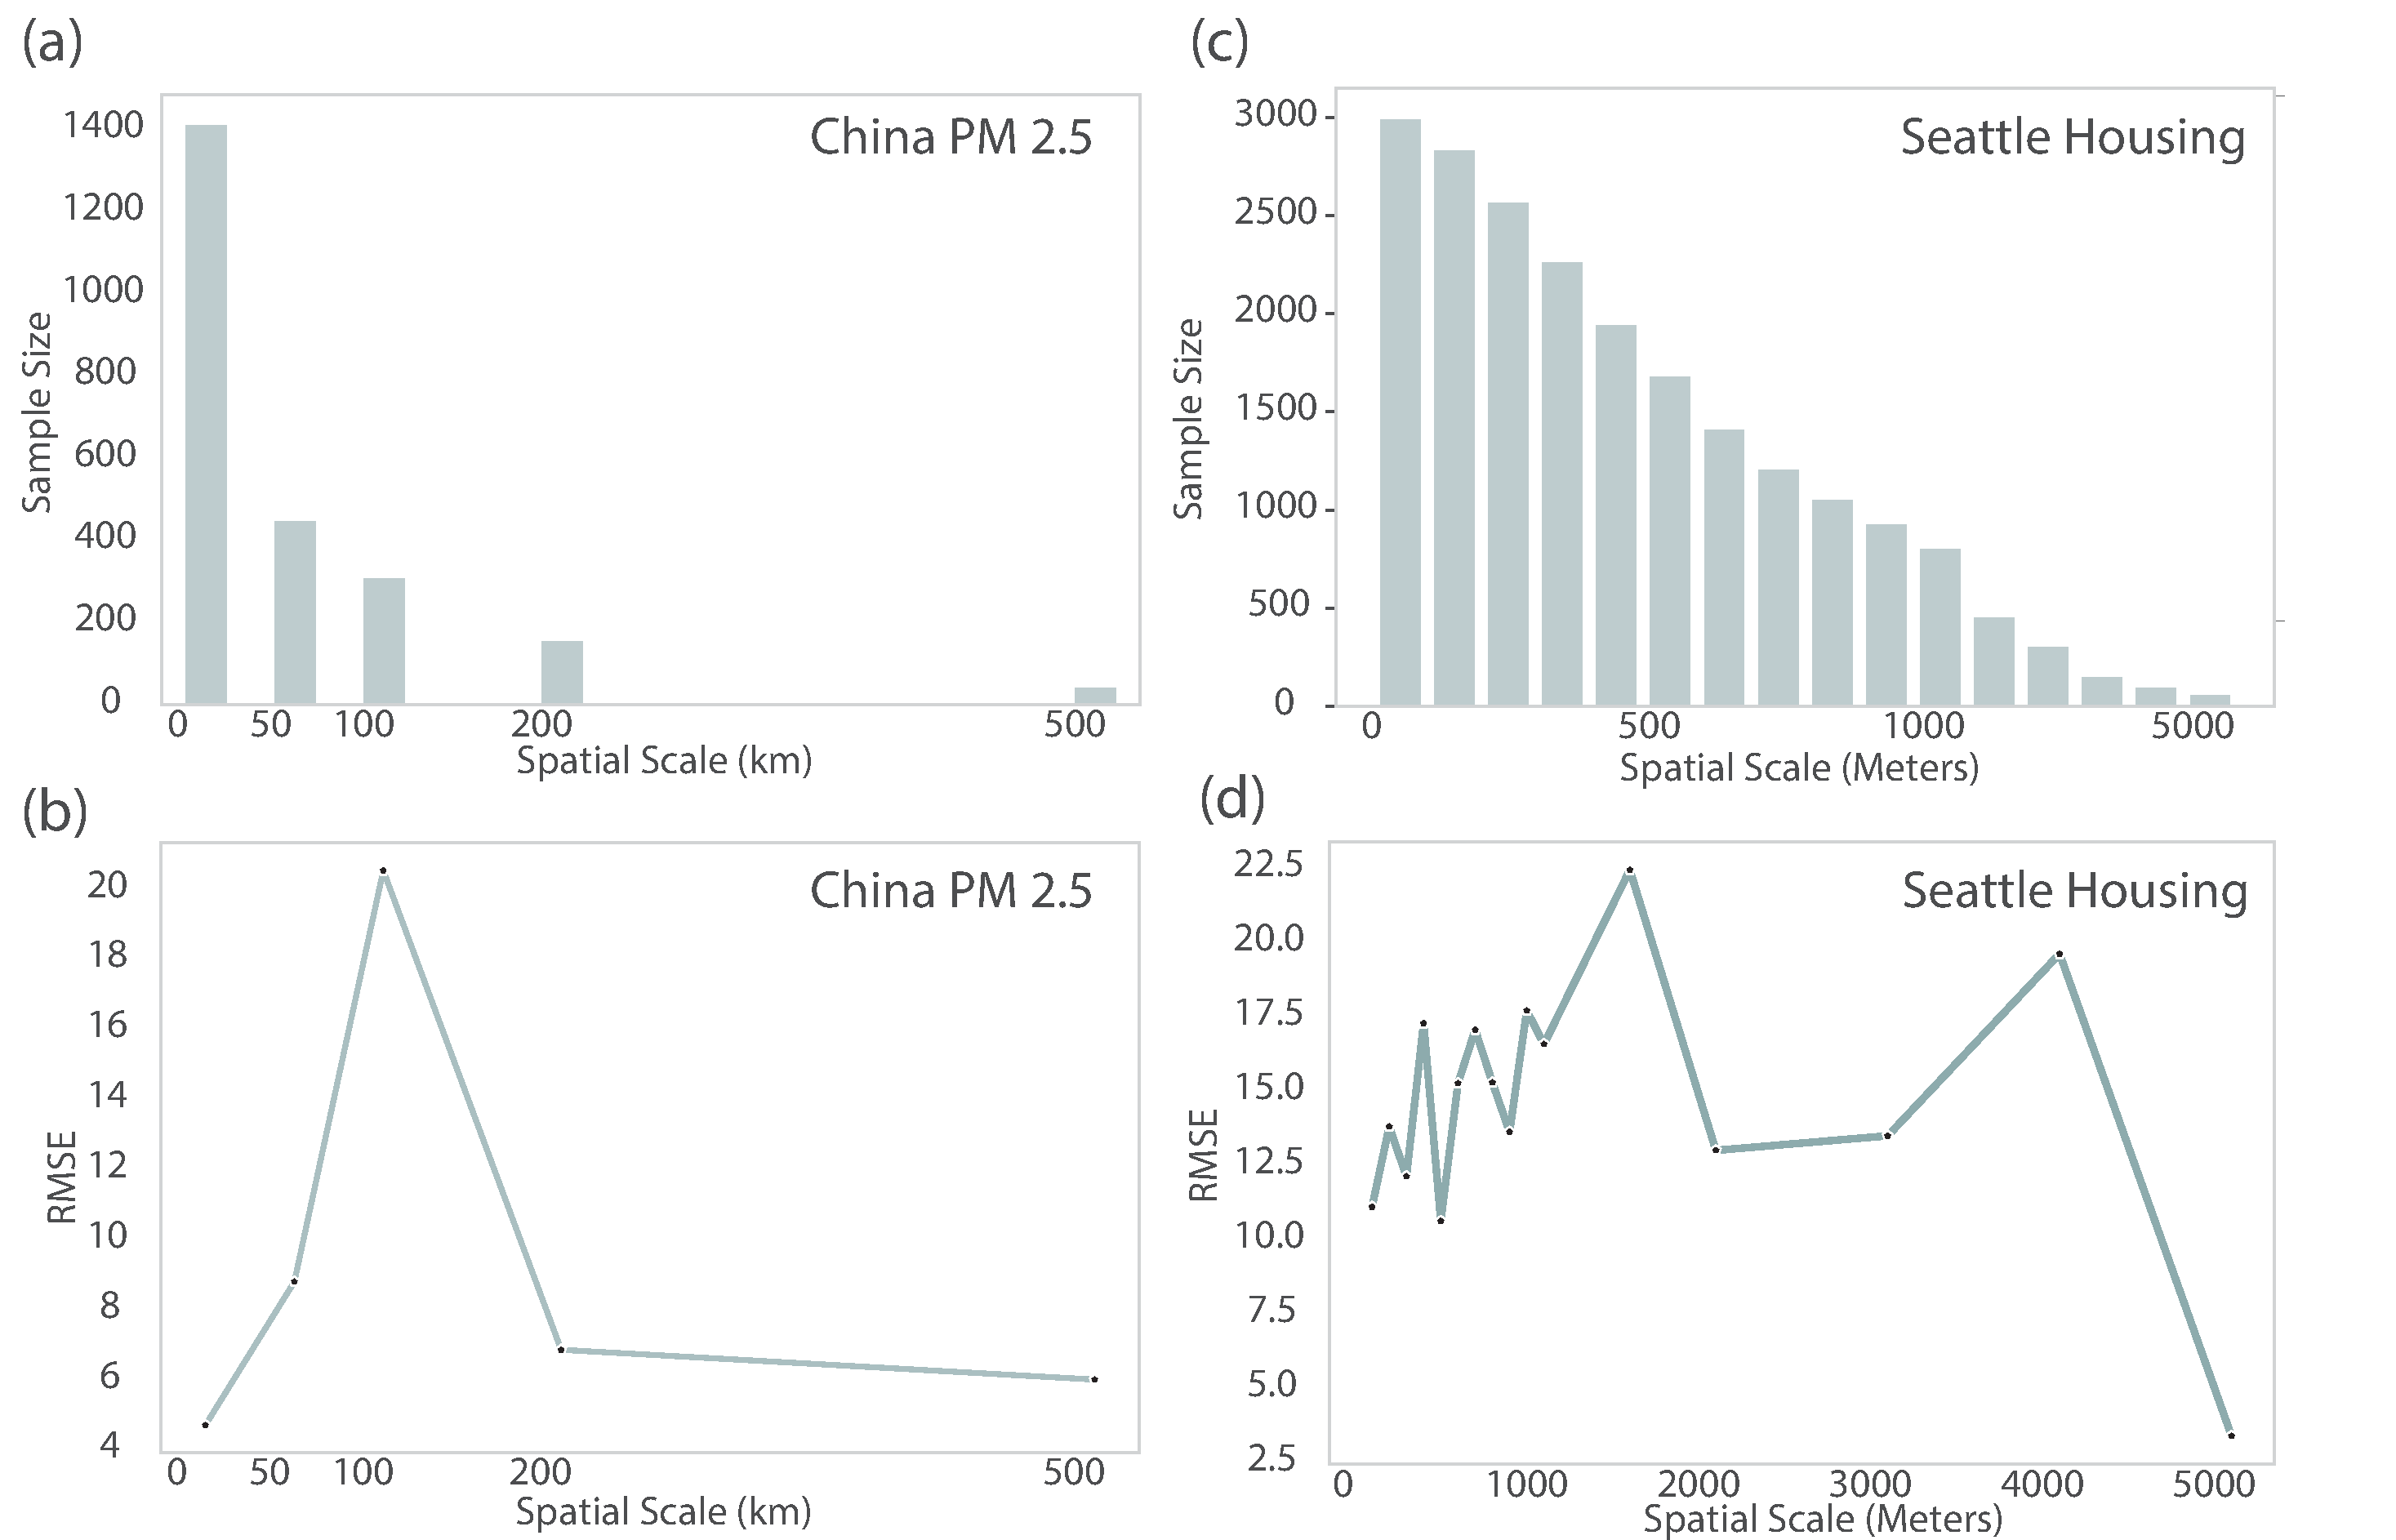
\includegraphics[width=1\linewidth]{Figures/Figure_X_Scele_2.pdf}
    \caption{Impact of spatial aggregation on effective sample size and predictive performance.}
    \label{fig:scale_1}
\end{figure*}



Figure~\ref{fig:scale_2} illustrates the uncertainty quantification (UQ) performance of GeoCP and GeoSIMCP variants across various spatial aggregation scales, using the China PM$_{2.5}$ and Seattle Housing datasets. The top panels (Figures~\ref{fig:scale_2}a and \ref{fig:scale_2}c) display the Interval Scores, while the bottom panels (Figures~\ref{fig:scale_2}b and \ref{fig:scale_2}d) present the Mean Interval Width. In these visualizations, the line plots track the absolute metrics for each model, whereas the overlaid bar charts quantify the relative improvement of GeoSIMCP over GeoCP. Notably, positive values in the bar charts signify a performance gain, indicating that GeoSIMCP achieves more refined and accurate uncertainty estimates.

For the China PM$_{2.5}$ dataset, GeoSIMCP consistently achieves lower interval scores and narrower prediction intervals than GeoCP at most aggregation scales. These improvements indicate that GeoSIMCP is able to construct more informative uncertainty intervals without sacrificing calibration, even as spatial aggregation reduces sample size and smooths local variability. 

For the Seattle Housing dataset, the relative performance of GeoSIMCP varies more substantially across spatial scales. At small to moderate aggregation distances (below approximately 1,000--1,500\,m), GeoSIMCP generally yields lower interval scores and narrower intervals than GeoCP, indicating improved UQ performance. However, at larger aggregation scales, the improvements become less stable, with several scales showing marginal gains or slight degradations relative to GeoCP. This variability reflects the combined effects of decreasing sample size, increased within-cell heterogeneity, and changes in feature-space structure induced by spatial aggregation. 

Overall, these results demonstrate that GeoSIMCP maintains effective uncertainty quantification performance across a wide range of spatial scales. By jointly leveraging geographic and feature-space similarity, GeoSIMCP is able to adapt to the statistical distortions introduced by the scale effect. 

\begin{figure*}[htbp]
    \centering
    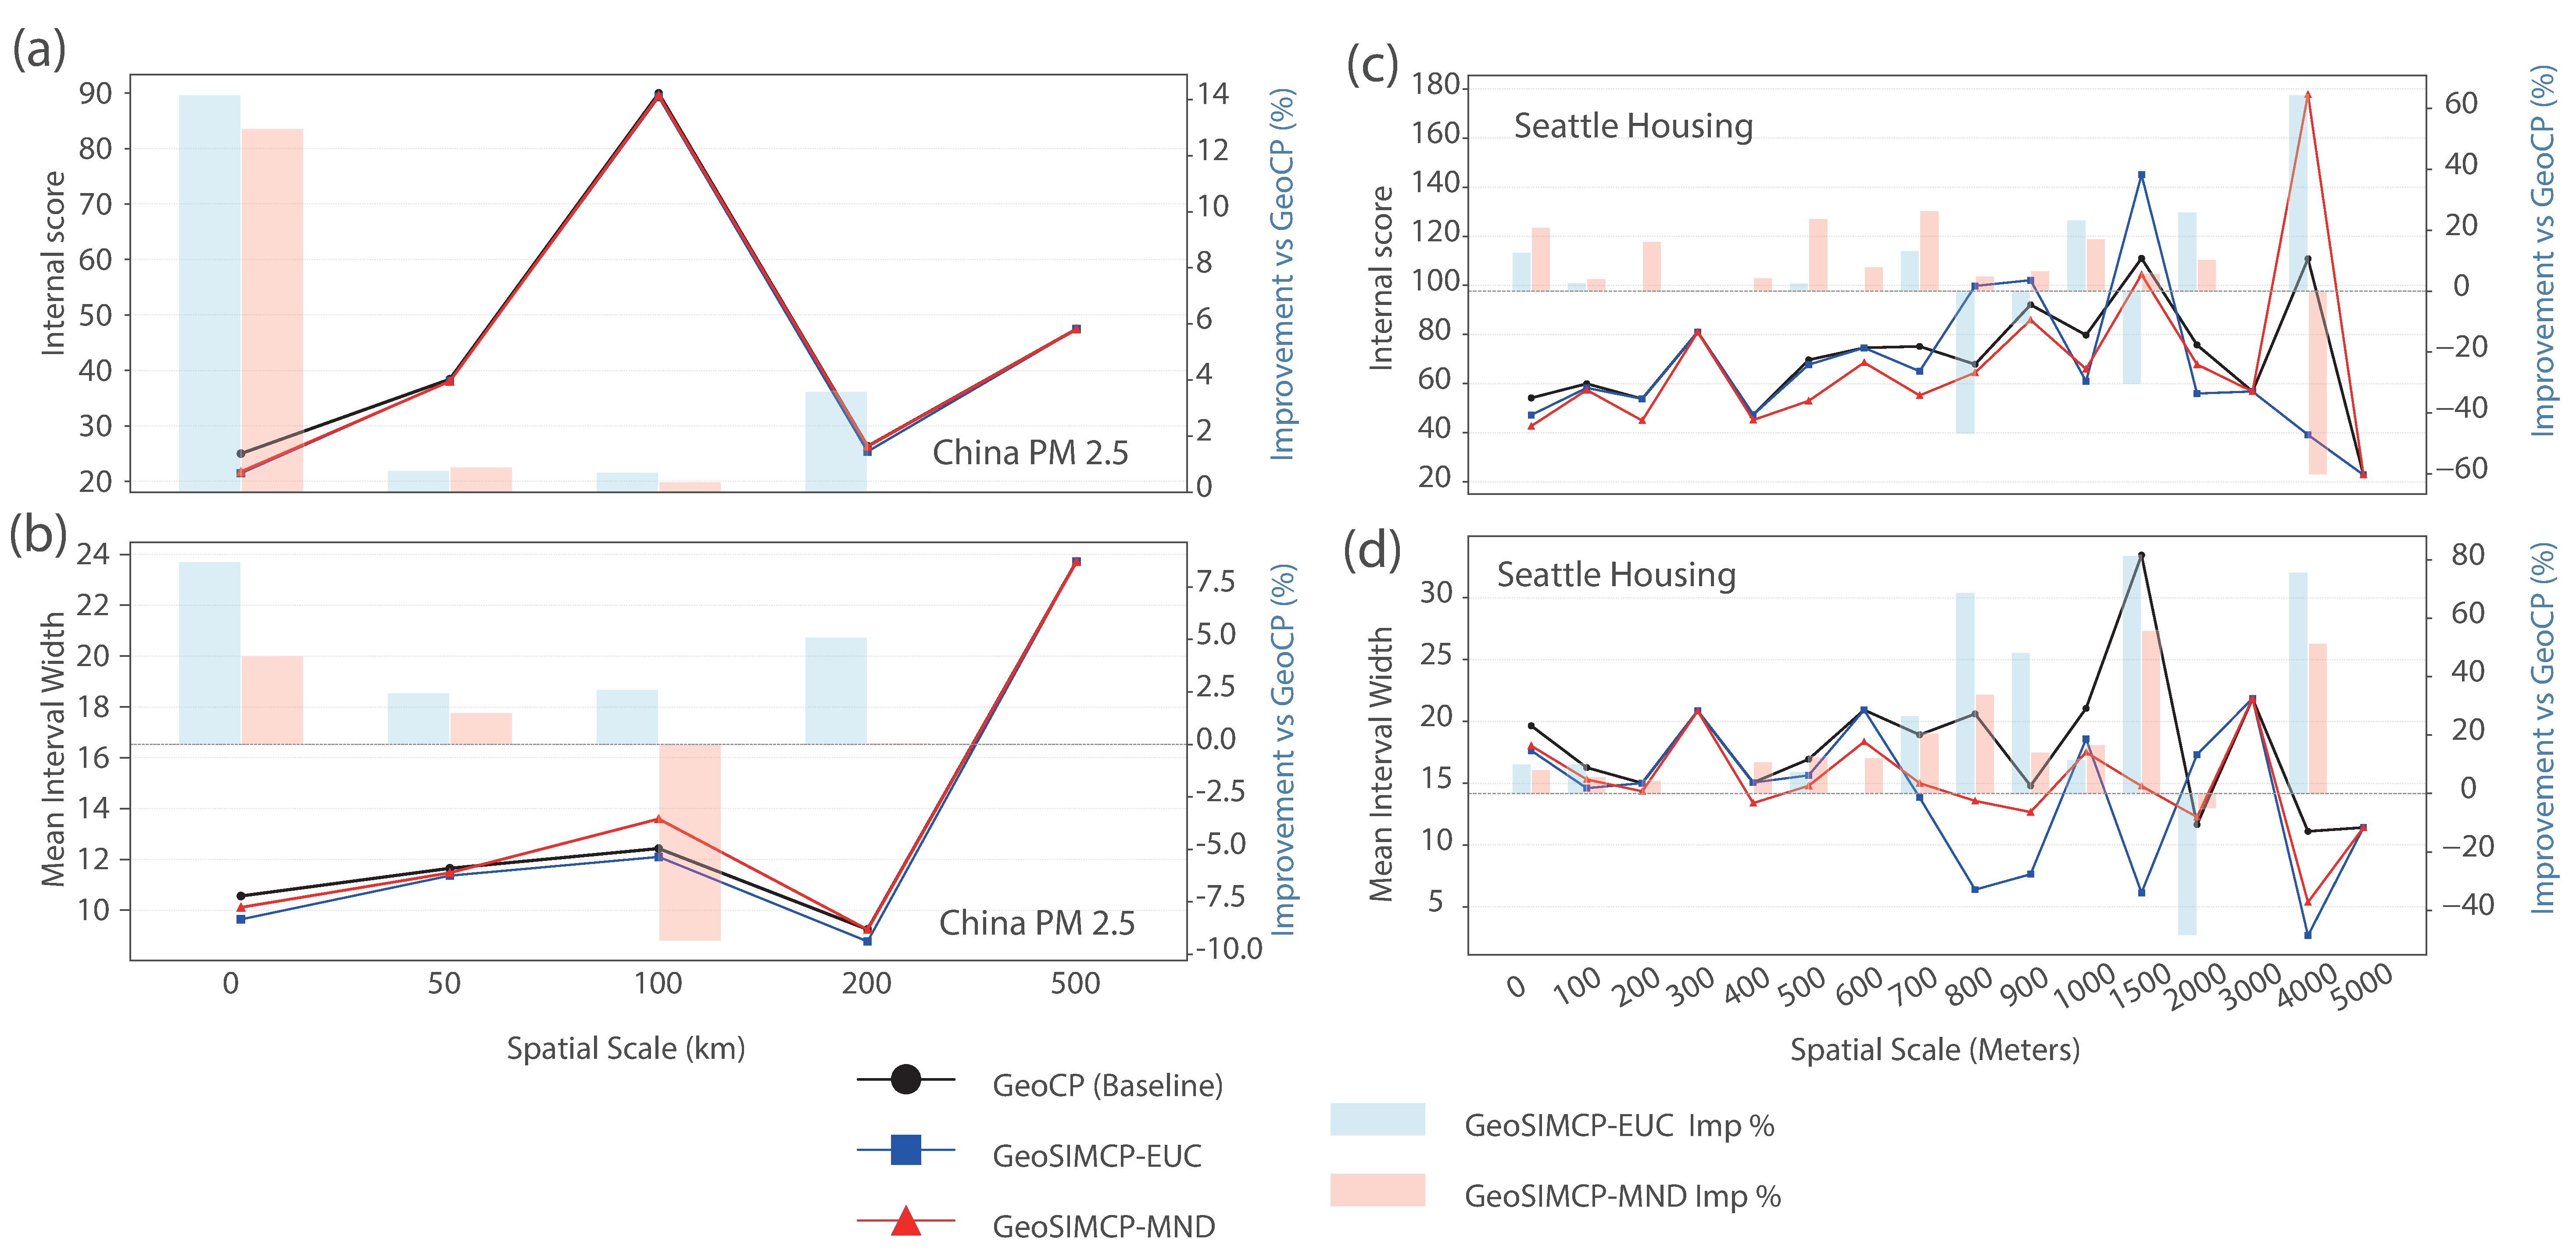
\includegraphics[width=1\linewidth]{Figures/Figure_X_Scele_1.pdf}
    \caption{Uncertainty quantification performance across increasing spatial aggregation scales.}
    \label{fig:scale_2}
\end{figure*}


Figure \ref{fig:maup} presents the interval score of UQ models at the MAUP experiment results for the China PM${2.5}$ and Seattle Housing datasets, under repeated zoning configurations (20 times). For each configuration, the full modeling and uncertainty quantification pipeline was recalibrated, including base model retraining and joint optimization of the kernel bandwidth $b$ and trade-off parameter $\lambda$. 

As illustrated, GeoSIMCP-MND consistently outperforms both GeoSIMCP-EUC and GeoCP across both datasets in terms of lower interval scores. This superiority highlights the critical importance of employing adaptive, distribution-aware feature similarity to characterize heterogeneous urban environments. For the China PM$_{2.5}$ dataset (Figure~\ref{fig:maup}a), GeoCP exhibits pronounced instability across different zoning configurations. This sensitivity suggests that GeoCP's performance is heavily influenced by boundary definitions, a classic manifestation of the \textbf{Modifiable Areal Unit Problem (MAUP)}. In contrast, both GeoSIMCP variants significantly reduce variability across trials, indicating that incorporating feature-space similarity enhances the robustness of localized exchangeability against zoning perturbations. Interestingly, for the Seattle Housing dataset, GeoSIMCP-EUC shows increased variability across zoning trials. This is likely attributable to feature-space distortion introduced by spatial aggregation, which complicates the distance metric's ability to maintain a consistent representation of spatial non-stationarity.

Overall, these results demonstrate that GeoSIMCP is more robust to the MAUP than GeoCP. By jointly leveraging geographic and feature-space similarity and fully recalibrating model parameters at each spatial configuration, GeoSIMCP maintains stable uncertainty estimates across zoning effects.

\begin{figure*}[htbp]
    \centering
    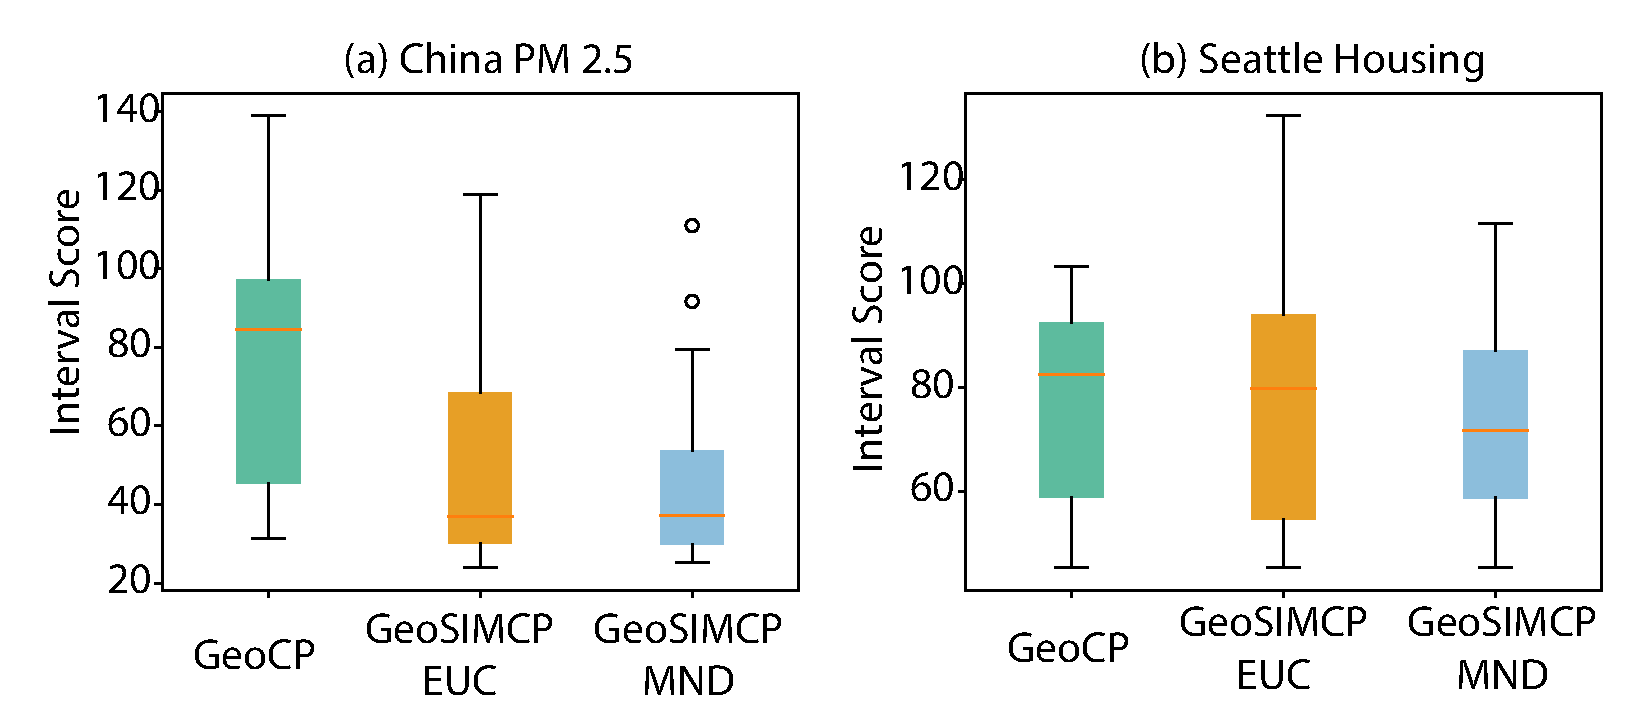
\includegraphics[width=1\linewidth]{Figures/Figure_X_MAUP.pdf}
    \caption{Impact of the MAUP on uncertainty quantification.}
    \label{fig:maup}
\end{figure*}




\subsubsection{Performance under spatial leave one out}


We partitioned the study areas using K-means clustering, with the optimal cluster counts—12 for the China dataset and 10 for Seattle—determined by the Elbow Method. To evaluate the UQ models' performance, we implemented a spatial leave-one-out validation strategy. 

As illustrated in Figure~\ref{fig:leave_one_china}a, the regional RMSE map reveals pronounced spatial heterogeneity in predictive performance, with substantially lower errors in western and peripheral regions compared to eastern China. Regarding uncertainty quantification, GeoSIMCP-MND achieves the lowest median interval score (Figure~\ref{fig:leave_one_china}b), effectively balancing interval width with improved coverage. In contrast, GeoCP exhibits significantly higher scores driven by poor coverage and large penalty terms. These results suggest that under spatial extrapolation, feature-informed uncertainty estimates are more robust than overconfident, spatially localized ones.

While GeoSIMCP—particularly the MND variant—yields wider intervals than GeoCP (Figure~\ref{fig:leave_one_china}c), this conservatism is an appropriate response to the absence of local training data in held-out regions. Conversely, GeoCP generates narrower intervals despite the lack of spatial support, indicating overconfidence under extrapolation. This behavior is confirmed by the coverage results (Figure~\ref{fig:leave_one_china}d). GeoCP suffers from severe undercoverage, demonstrating a breakdown of its localized exchangeability assumption when spatial proximity between training and test samples is absent. While GeoSIMCP-EUC offers modest improvements, it remains undercalibrated. GeoSIMCP-MND achieves the highest and most stable coverage, indicating that feature-space similarity partially restores exchangeability even when geographic neighbors are unavailable.



\begin{figure*}[htbp]
    \centering
    \includegraphics[width=1\linewidth]{Figures/Figure_X_leave_one_China.pdf}
    \caption{Uncertainty quantification under spatial leave-one-out extrapolation for the China PM$_{2.5}$ dataset.}
    \label{fig:leave_one_china}
\end{figure*}



Figure~\ref{fig:leave_one_seattle} presents the uncertainty quantification results for the Seattle Housing dataset under the spatial leave-one-out setting. The regional RMSE map (Figure~\ref{fig:leave_one_seattle}a) reveals distinct spatial patterns in prediction errors, with significantly higher errors observed in the northern regions of Seattle during leave-one-out cross-validation. This suggests that northern areas possess unique \textbf{local spatial signatures} that are not easily captured by the data distributions of other regions.

The interval score distributions (Figure~\ref{fig:leave_one_seattle}b) indicate that GeoSIMCP substantially outperforms GeoCP in this spatial extrapolation scenario. GeoCP yields the highest median interval scores, a result of its excessively narrow prediction intervals coupled with severe undercoverage. While GeoSIMCP-EUC reduces interval scores compared to GeoCP, it exhibits considerable cross-regional variability. This suggests a sensitivity to \textbf{feature-space distortions} induced by spatial aggregation and heterogeneity. In contrast, GeoSIMCP-MND achieves the lowest median interval score with tight dispersion, demonstrating more efficient and robust uncertainty quantification.

This performance gain is driven by wider, more representative prediction intervals (Figure~\ref{fig:leave_one_seattle}c), which appropriately reflect the increased epistemic uncertainty when predicting housing prices in unseen urban sub-markets. Importantly, this calibration leads to substantially improved coverage. While GeoCP fails to provide meaningful coverage in most held-out regions and GeoSIMCP-EUC displays unstable calibration, GeoSIMCP-MND consistently maintains coverage levels near the nominal threshold across various spatial clusters (Figure~\ref{fig:leave_one_seattle}d).

Overall, these results demonstrate that for highly heterogeneous urban datasets, uncertainty quantification under spatial extrapolation critically depends on the ability to leverage feature-space similarity beyond geographic proximity. By incorporating an adaptive, feature-aware similarity metric, GeoSIMCP-MND provides more reliable and honest uncertainty estimates than purely geography-based conformal prediction, particularly in settings where spatial neighbors are unavailable.


\begin{figure*}[htbp]
    \centering
    \includegraphics[width=1\linewidth]{Figures/Figure_X_leave_one_Seattle.pdf}
    \caption{Uncertainty quantification under spatial leave-one-out extrapolation for the Seattle housing dataset.}
    \label{fig:leave_one_seattle}
\end{figure*}


}


\section{Discussion}

This work proposes a model-agnostic framework for uncertainty quantification in spatial prediction, building upon GeoCP, but designed to handle spatially nonstationary processes. GeoCP is the first model-agnostic framework for uncertainty quantification in spatial prediction. Owing to its simple assumption—namely, the spatial dependence of geographic processes—it can be effectively applied to spatial prediction tasks without explanatory variables, such as spatial interpolation. However, real-world geographic processes are often non-stationary, making it unreliable to measure similarity between locations based solely on geographic distance. To address this limitation, we propose GeoSIMCP as an extension of GeoCP. In scenarios where high-quality explanatory variables are available—such as spatial regression—GeoSIMCP incorporates geographic configuration similarity to better reflect the underlying process similarity between locations. When no explanatory variables are available, GeoSIMCP naturally degenerates to GeoCP.

We designed a series of simulation experiments involving 324 spatial prediction scenarios with uncertainty, generated under varying levels of spatial and feature-space noise smoothness and intensity. These experiments demonstrate that GeoSIMCP consistently outperforms GeoCP by achieving higher coverage with narrower prediction intervals. We further validated the superiority of GeoSIMCP on two real-world datasets: housing prices and China’s PM2.5 concentrations.


However, there are some limitations of GeoSIMCP. First, the weighting scheme between geographic and feature-space distances has the potential to be improved. \textcolor{red}{The parameter $\lambda$ is introduced to facilitate localized exchangeability in conformal prediction by balancing the influence of geographic proximity and feature similarity. It is therefore a methodological tuning parameter, rather than one with a direct theoretical or physical interpretation.} Our motivation is to provide an efficient and interpretable solution, as the trade-off parameter $\lambda$ offers insight into the geographic process underlying the target variable—i.e., the extent to which prediction is influenced by spatial dependence. However, such a linear combination of distances may lead to suboptimal weighting when the two types of distances are not directly comparable in scale, or when their influence on prediction is nonlinearly entangled. This simplification may limit the model’s flexibility in capturing complex spatial interactions or heterogeneous spatial processes where the relative importance of geographic versus feature similarity varies across space.

Second, we applied $z$-score normalization to the feature-space distances to ensure that their magnitudes are comparable across dimensions, but we did not normalize the geographic distances. This design choice was based on the fact that geographic coordinates have inherent physical meaning—such as degrees or kilometers—and their raw scale reflects real-world spatial extents. Moreover, by tuning the trade-off parameter $\lambda$, we aim to balance the influence between geographic and feature distances, thereby partially mitigating their scale mismatch. Nonetheless, this asymmetric treatment may still introduce unintended biases, especially when the magnitude ranges of the two types of distances differ substantially. In such cases, the kernel weighting function may disproportionately emphasize one domain over the other. Future extensions could consider jointly standardizing or adaptively rescaling both distance components based on empirical distributions.

Third, in GeoSIMCP, a global bandwidth parameter is applied uniformly across the entire spatial domain when computing the kernel-based weights between each test sample and the calibration set. This fixed bandwidth does not account for local density variations or spatial heterogeneity, which may limit the model’s ability to adapt to region-specific uncertainty structures.






\section{Conclusion}

This study proposes a new model for quantifying the uncertainty of spatial prediction models while accounting for nonstationary spatial processes. We incorporate feature similarity into geospatial conformal prediction through the development of GeoSIMCP. The performance of GeoSIMCP is evaluated using simulation experiments and two sets of real-world datasets. The results demonstrate that GeoSIMCP is able to provide more accurate prediction intervals with narrower widths compared with existing spatial uncertainty quantification models. Future work may focus on improving the weighting scheme for geographic distance and feature similarity, as well as developing adaptive methods for selecting location-specific bandwidths.

% \section{Data available statement}

% The data and codes that support the findings of the present study are available on Figshare at https://figshare.com/s/852947942dcaa415cc3e.

\section{Disclosure Statement}

The authors declare no conflicts of interest. Generative AI (i.e., GPT-4o) was used for language editing and grammar checking, and was not employed to generate, expand, or alter the scientific ideas, data analyses, or conclusions.


\appendix
\renewcommand{\thefigure}{S\arabic{figure}}
\setcounter{figure}{0}


\section{Localized joint exchangeability and coverage validity in GeoSIMCP}


 
\textcolor{red}{We formalize the coverage guarantee of GeoSIMCP by adopting a localized, similarity-weighted form of exchangeability. This assumption follows the standard weighted conformal prediction framework, in which samples are not required to be globally exchangeable, but are assumed to be exchangeable after reweighting according to their similarity to the test point.}


\textbf{Assumption (Localized joint weighted exchangeability).}  
Let \(Z_i = (X_i, y_i)\) for \(i=1, \dots, n+1\), where each \(X_i\) contains both geographic coordinates and feature-space attributes. We define a nonnegative, measurable weight function that assigns higher importance to samples close to the test location in a combined feature-geographic space.  

We assume that the joint distribution of \((Z_1, \dots, Z_{n+1})\) satisfies a localized weighted exchangeability condition around the test point \(X_{n+1}\), formally:


\begin{equation} P((Z_1, \dots, Z_{n+1}) \in A) = E\left[ \frac{ \prod_{i=1}^{n+1} w(X_{\pi(i)}) }{ \sum_{i=1}^{n+1} w(X_{\pi(i)}) } \cdot \mathbb{I}{(Z_1, \dots, Z_{n+1}) \in A} \right], 
\end{equation}

for all measurable sets \(A\) and all permutations \(\pi\) of \(\{1, \dots, n+1\}\).

This assumption relaxes classical global exchangeability by focusing probability mass on samples that are jointly similar in location and features, thereby adapting to local heterogeneity in spatially structured data.

\vspace{0.5em}


When \(\lambda=1\), the joint distance reduces to pure geographic distance:

\[
d_{\text{joint}}(i) = d_{\text{geo}}(i),
\]

thus recovering the original GeoCP framework.  
GeoSIMCP can therefore be viewed as a strict generalization of GeoCP, allowing feature-space similarity to be flexibly integrated.


\textcolor{red}{The following coverage guarantee is a direct consequence of existing results on weighted conformal prediction and is stated here for completeness. Specifically, this result can be viewed as a localized instantiation of Theorem~2 in \citep{tibshirani2019conformal} under a similarity-induced weighting scheme, with additional spatial motivation discussed in \citet{lou2025geoxcp}.}

\textbf{Theorem (Localized coverage guarantee for GeoSIMCP).}  
Under the localized joint weighted exchangeability assumption, define the nonconformity scores \(\alpha_i = \alpha(X_i, y_i)\) for \(i = 1, \dots, n\), and compute normalized weights:

\begin{equation}
\hat{w}_i = \frac{w(X_i)}{\sum_{j=1}^{n+1} w(X_j)}.
\end{equation}

Let the weighted quantile threshold be determined by:

% \begin{equation}
% t_{1-\alpha}(X_{n+1}) = \inf\left\{t : \sum_{i=1}^{n} \hat{w}_i \mathbf{1}\{\alpha_i \leq t\} \geq 1-\alpha \right\},
% \end{equation}

\begin{equation}
t_{1-\alpha}(X_{n+1}) = \inf \left\{ t : \sum_{i=1}^{n} \hat{w}_i \mathbb{I} \{ \alpha_i \leq t \} \geq 1-\alpha \right\}
\end{equation}

and define the prediction set:

\begin{equation}
C(X_{n+1}) = \{ y : \alpha(X_{n+1}, y) \leq t_{1-\alpha}(X_{n+1})\}.
\end{equation}

Then, the conformal prediction interval constructed via GeoSIMCP satisfies:

\begin{equation}
P\left( Y_{n+1} \in C(X_{n+1}) \right) \geq 1 - \alpha.
\end{equation}

Thus, despite incorporating joint feature--geographic adaptivity, GeoSIMCP retains a formal marginal coverage guarantee analogous to classical conformal prediction under mild localized sampling assumptions. 
\textcolor{red}{This guarantee is marginal and holds in finite samples whenever the localized weighted exchangeability assumption is satisfied, consistent with existing results in the conformal prediction literature.}


\section{Spatial regime noise}

{
\color{red}

\subsection{Experiments} 

To examine the behavior of conformal prediction under spatial processes with abrupt structural changes, we design a simulation in which noise follows a regime-based spatial pattern with explicit boundaries. The goal of this experiment is not to compare different uncertainty quantification models, but to probe how conformal prediction responds to spatial non-smoothness induced by regime shifts.

Let the spatial domain be represented by a regular grid, where each location is associated with a spatial coordinate $\mathbf{s}_i = (Lon_i, Lat_i)$. The domain is partitioned into $R$ contiguous spatial regimes by thresholding one spatial dimension (e.g., the $x$-axis), resulting in a regime assignment
\begin{equation}
r(\mathbf{s}_i) \in \{1, \dots, R\}.
\end{equation}
Each regime corresponds to a spatially coherent subregion with a distinct noise-generating mechanism.

For each regime $r$, noise is sampled independently from a Gaussian distribution with regime-specific variance,
\begin{equation}
\varepsilon_i^{(r)} \sim \mathcal{N}(0, \sigma_r^2),
\end{equation}
where $\sigma_r$ controls the noise magnitude within regime $r$. To preserve local spatial coherence while maintaining sharp regime boundaries, Gaussian smoothing is applied only within each regime,
\begin{equation}
\tilde{\varepsilon}^{(r)}(\mathbf{s}) = \big(K_\sigma * \varepsilon^{(r)}\big)(\mathbf{s}), \quad \mathbf{s} \in r,
\end{equation}
where $K_\sigma$ denotes an isotropic Gaussian kernel and convolution is restricted to locations belonging to the same regime. No smoothing is performed across regime boundaries, ensuring abrupt changes in noise structure between adjacent regions.

The resulting regime-based noise field depends solely on spatial location and is independent of any feature-space variables. This noise is added to the underlying signal to generate observations governed by a spatial process with regime-dependent heteroskedasticity and discontinuities. Because the spatial regimes are defined purely in geographic space, uncertainty quantification methods that differ only in their use of feature-space similarity are theoretically expected to exhibit comparable behavior in this setting. Accordingly, this experiment serves as a diagnostic analysis of conformal prediction under spatial regime shifts, rather than a benchmark for model comparison.

\subsection{Results}

Figure \ref{fig:regime_noise} further reveals a consistent behavior of conformal prediction under spatial regime noise across different levels of noise smoothness. Regardless of whether the noise field is highly irregular or strongly smoothed, both GeoCP and GeoSIMCP tend to produce relatively smooth uncertainty estimates, reflecting their shared reliance on geographic distance for uncertainty calibration. As a result, uncertainty surfaces do not reproduce fine-scale noise variability, but instead emphasize broader spatial structure.

Despite this smoothing tendency, clear spatial regime patterns remain evident in the uncertainty maps. Sharp transitions aligned with regime boundaries persist across all smoothness levels, indicating that conformal prediction effectively captures regime-level heterogeneity even when local variability is suppressed. This suggests that distance-based calibration is sensitive to large-scale spatial discontinuities, while being less responsive to high-frequency spatial noise.

Moreover, as the spatial noise becomes progressively smoother, the uncertainty estimates increasingly align with the true spatial pattern of prediction errors. Under higher smoothness, prediction errors exhibit stronger spatial coherence, and conformal prediction more faithfully reflects the underlying error structure. This trend highlights that conformal prediction is better suited to spatial processes that satisfy smoothness assumptions, while its response under highly irregular spatial noise is necessarily dominated by distance-based aggregation.



\begin{figure*}[htbp]
    \centering
    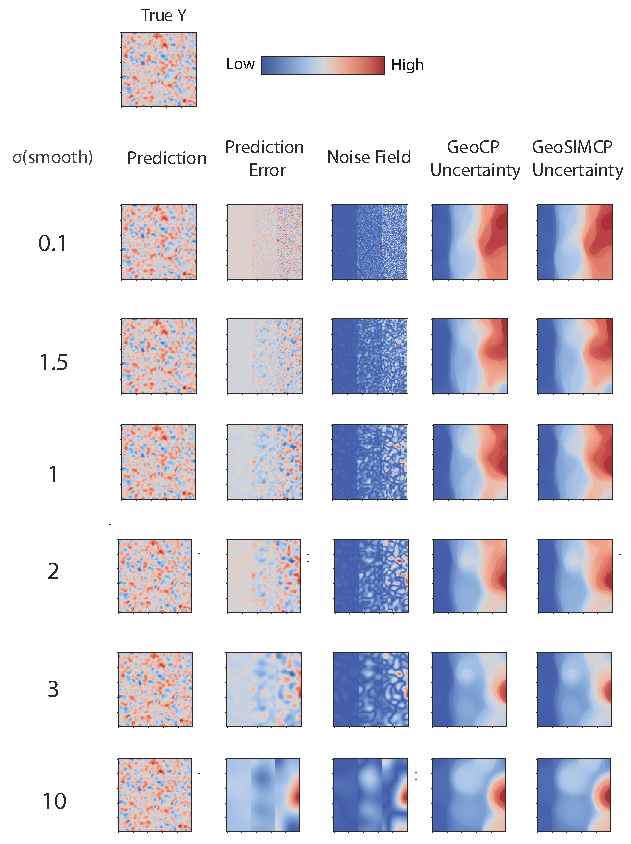
\includegraphics[width=1\linewidth]{Figures/Figure_X_uncertainty_mapping_regime_feature.pdf}
    \caption{The spatial uncertainty surfaces vary across different regimes of smoothed noise.}
    \label{fig:regime_noise}
\end{figure*}

}

\section{Parameter optimization process of real-data experiments}

Figures \ref{fig:appendix-pm2.5} and \ref{fig:appendix-housing} further illustrate the parameter optimization processes of these models in the tasks of PM2.5 prediction in China and housing price prediction in Seattle, respectively.

% Figure \ref{fig:interval_score_featurenoise} presents the average interval scores of the three models under different experimental settings. For each dataset, the best performance, indicated by the lowest interval score, is highlighted in bold.

% First, for all three models, the interval score decreases as the spatial correlation of the noise (i.e., noise sigma) increases. This suggests that noise with stronger spatial autocorrelation is easier to capture. In contrast, as the noise standard deviation increases, the interval score rises across all models, indicating that higher noise variance makes it more difficult for the conformal prediction-based models to generate intervals that successfully cover the true values.

% Second, when comparing GeoCP and GeoSIMCP, GeoSIMCP outperforms or matches GeoCP in all 162 experimental settings. The advantage is particularly pronounced when the noise sigma is small. For example, when the noise standard deviation is 10 and noise sigma is 0.1, the interval score of GeoCP is 9.61, significantly higher than 5.56 for GeoSIMCP- EUC, representing a 42.1% reduction, and 6.25 for GeoSIMCP- MND, representing a 34.9% reduction.

% Third, comparing the two variants of GeoSIMCP, GeoSIMCP- EUC achieves better performance when noise sigma is below 2.0, whereas GeoSIMCP- MND performs better when noise sigma exceeds 2.0.

% \begin{figure*}[htbp]
%     \centering
%     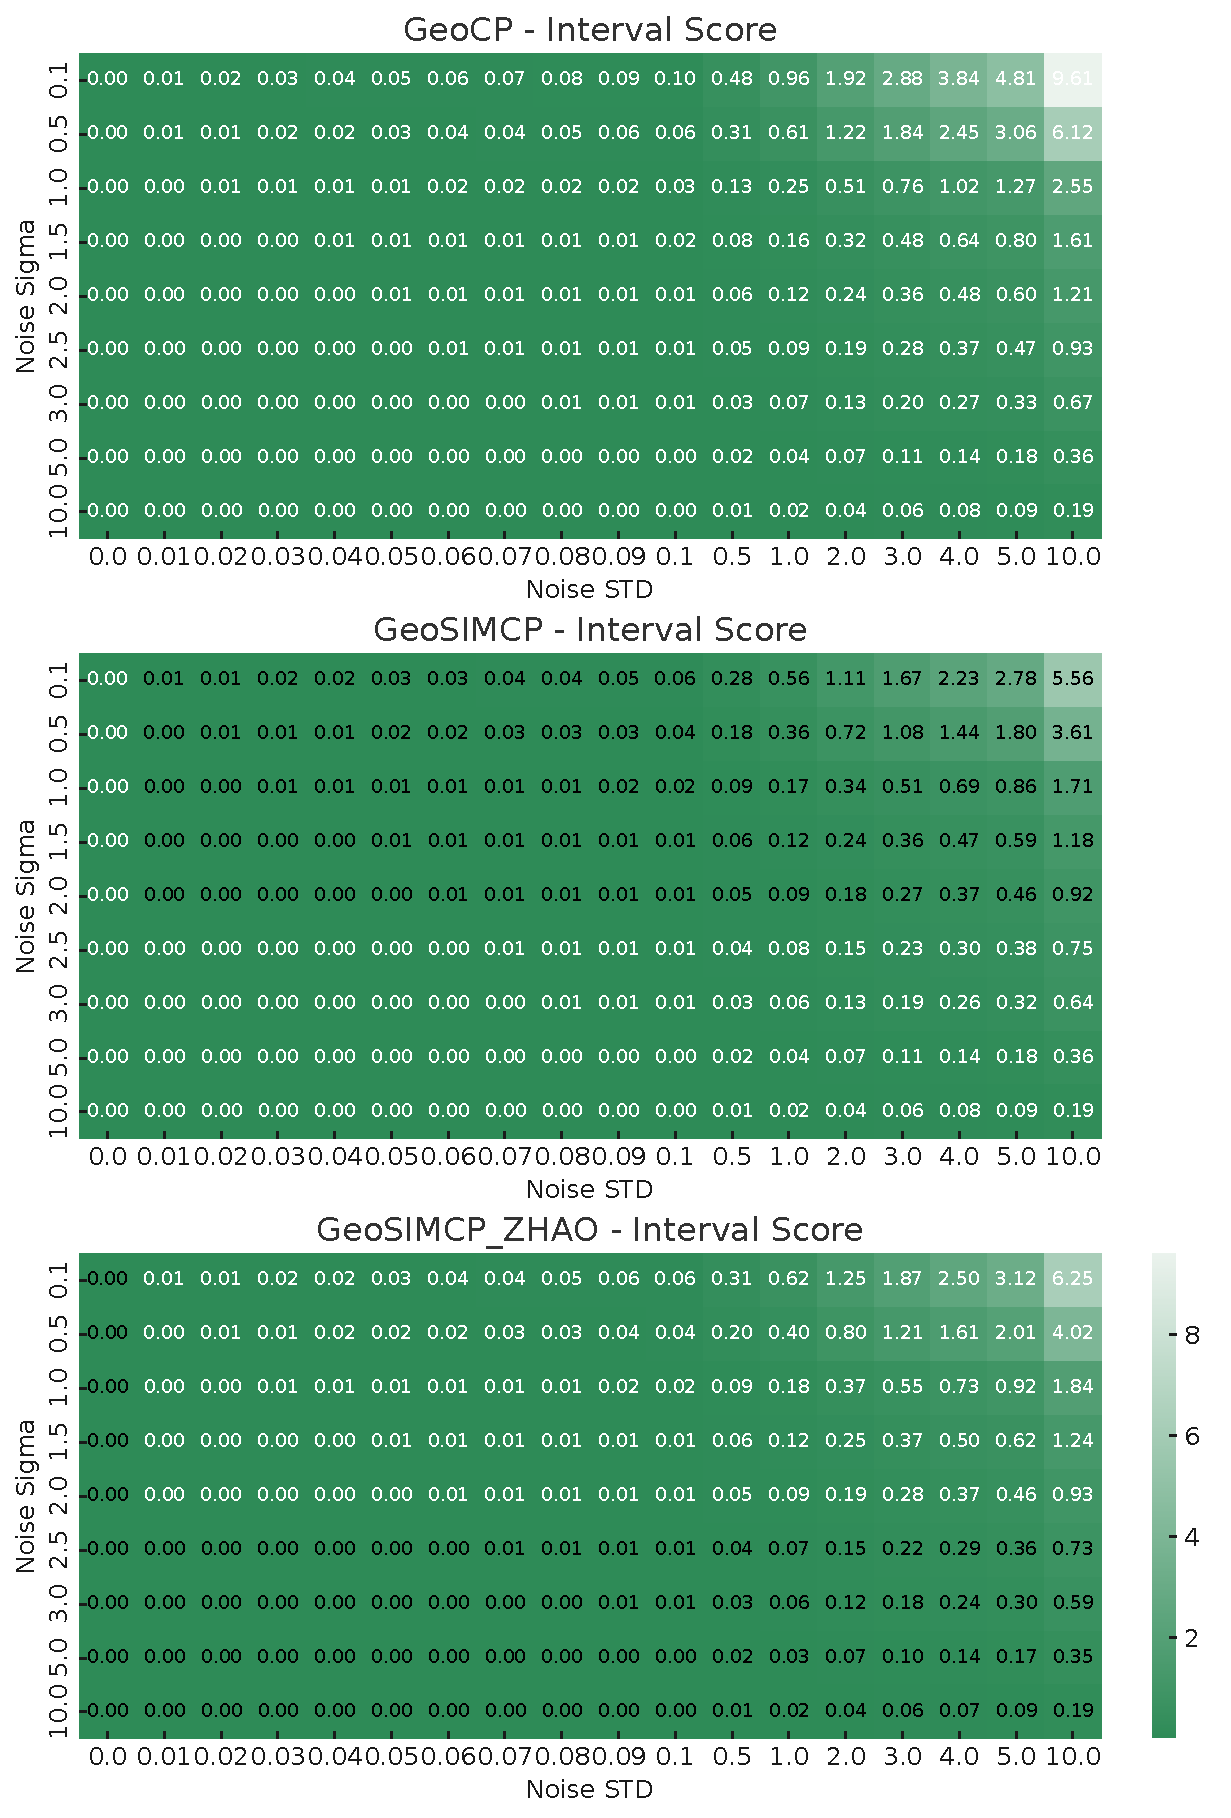
\includegraphics[width=1\linewidth]{Figures/FigureX_simu_interval_score.pdf}
%     \caption{Estimating the expectation value of explanation output}
%     \label{fig:interval_score_featurenoise}
% \end{figure*}


% \begin{figure*}[htbp]
%     \centering
%     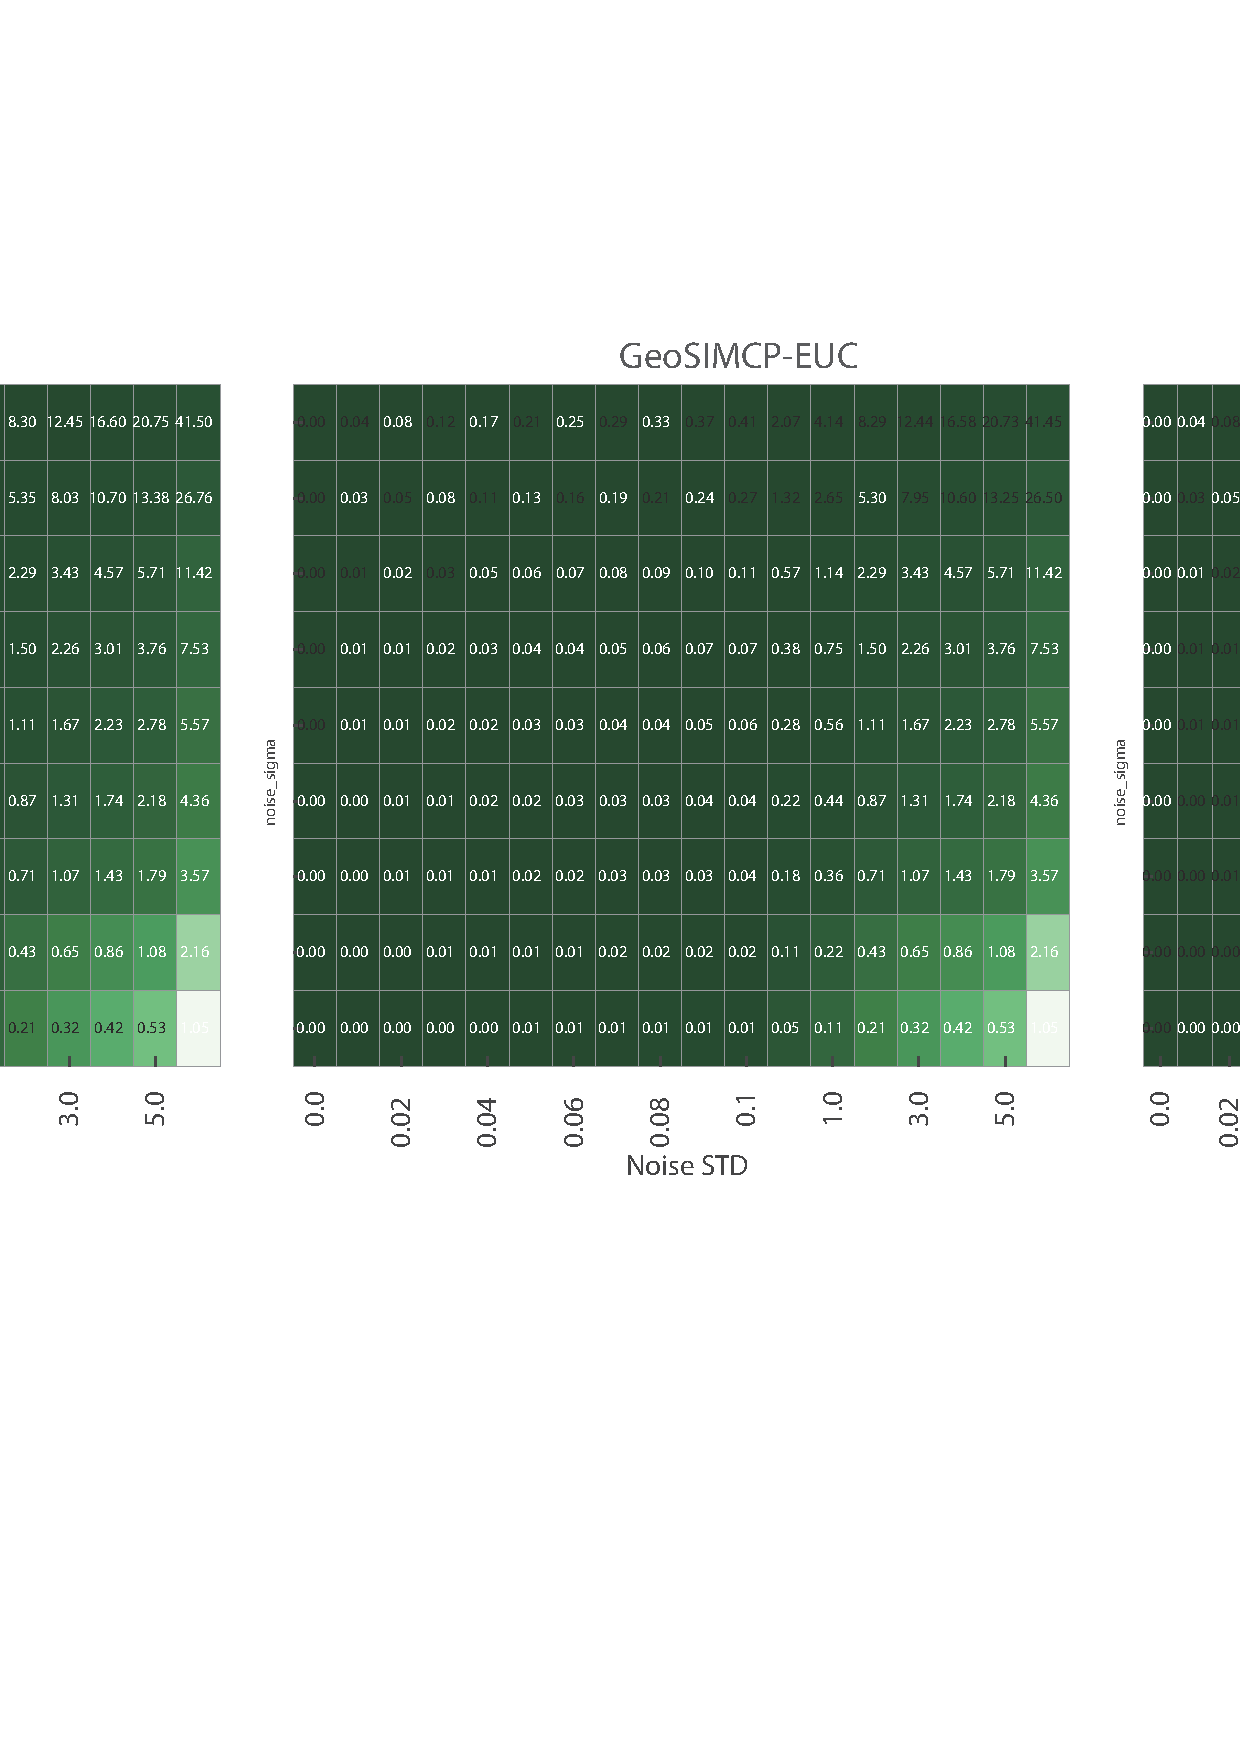
\includegraphics[width=1\linewidth]{Figures/FigureX_simu_interval_score_geonoise.pdf}
%     \caption{Estimating the expectation value of explanation output}
%     \label{fig:interval_score_featurenoise}
% \end{figure*}






% \begin{figure*}[htbp]
%     \centering
%     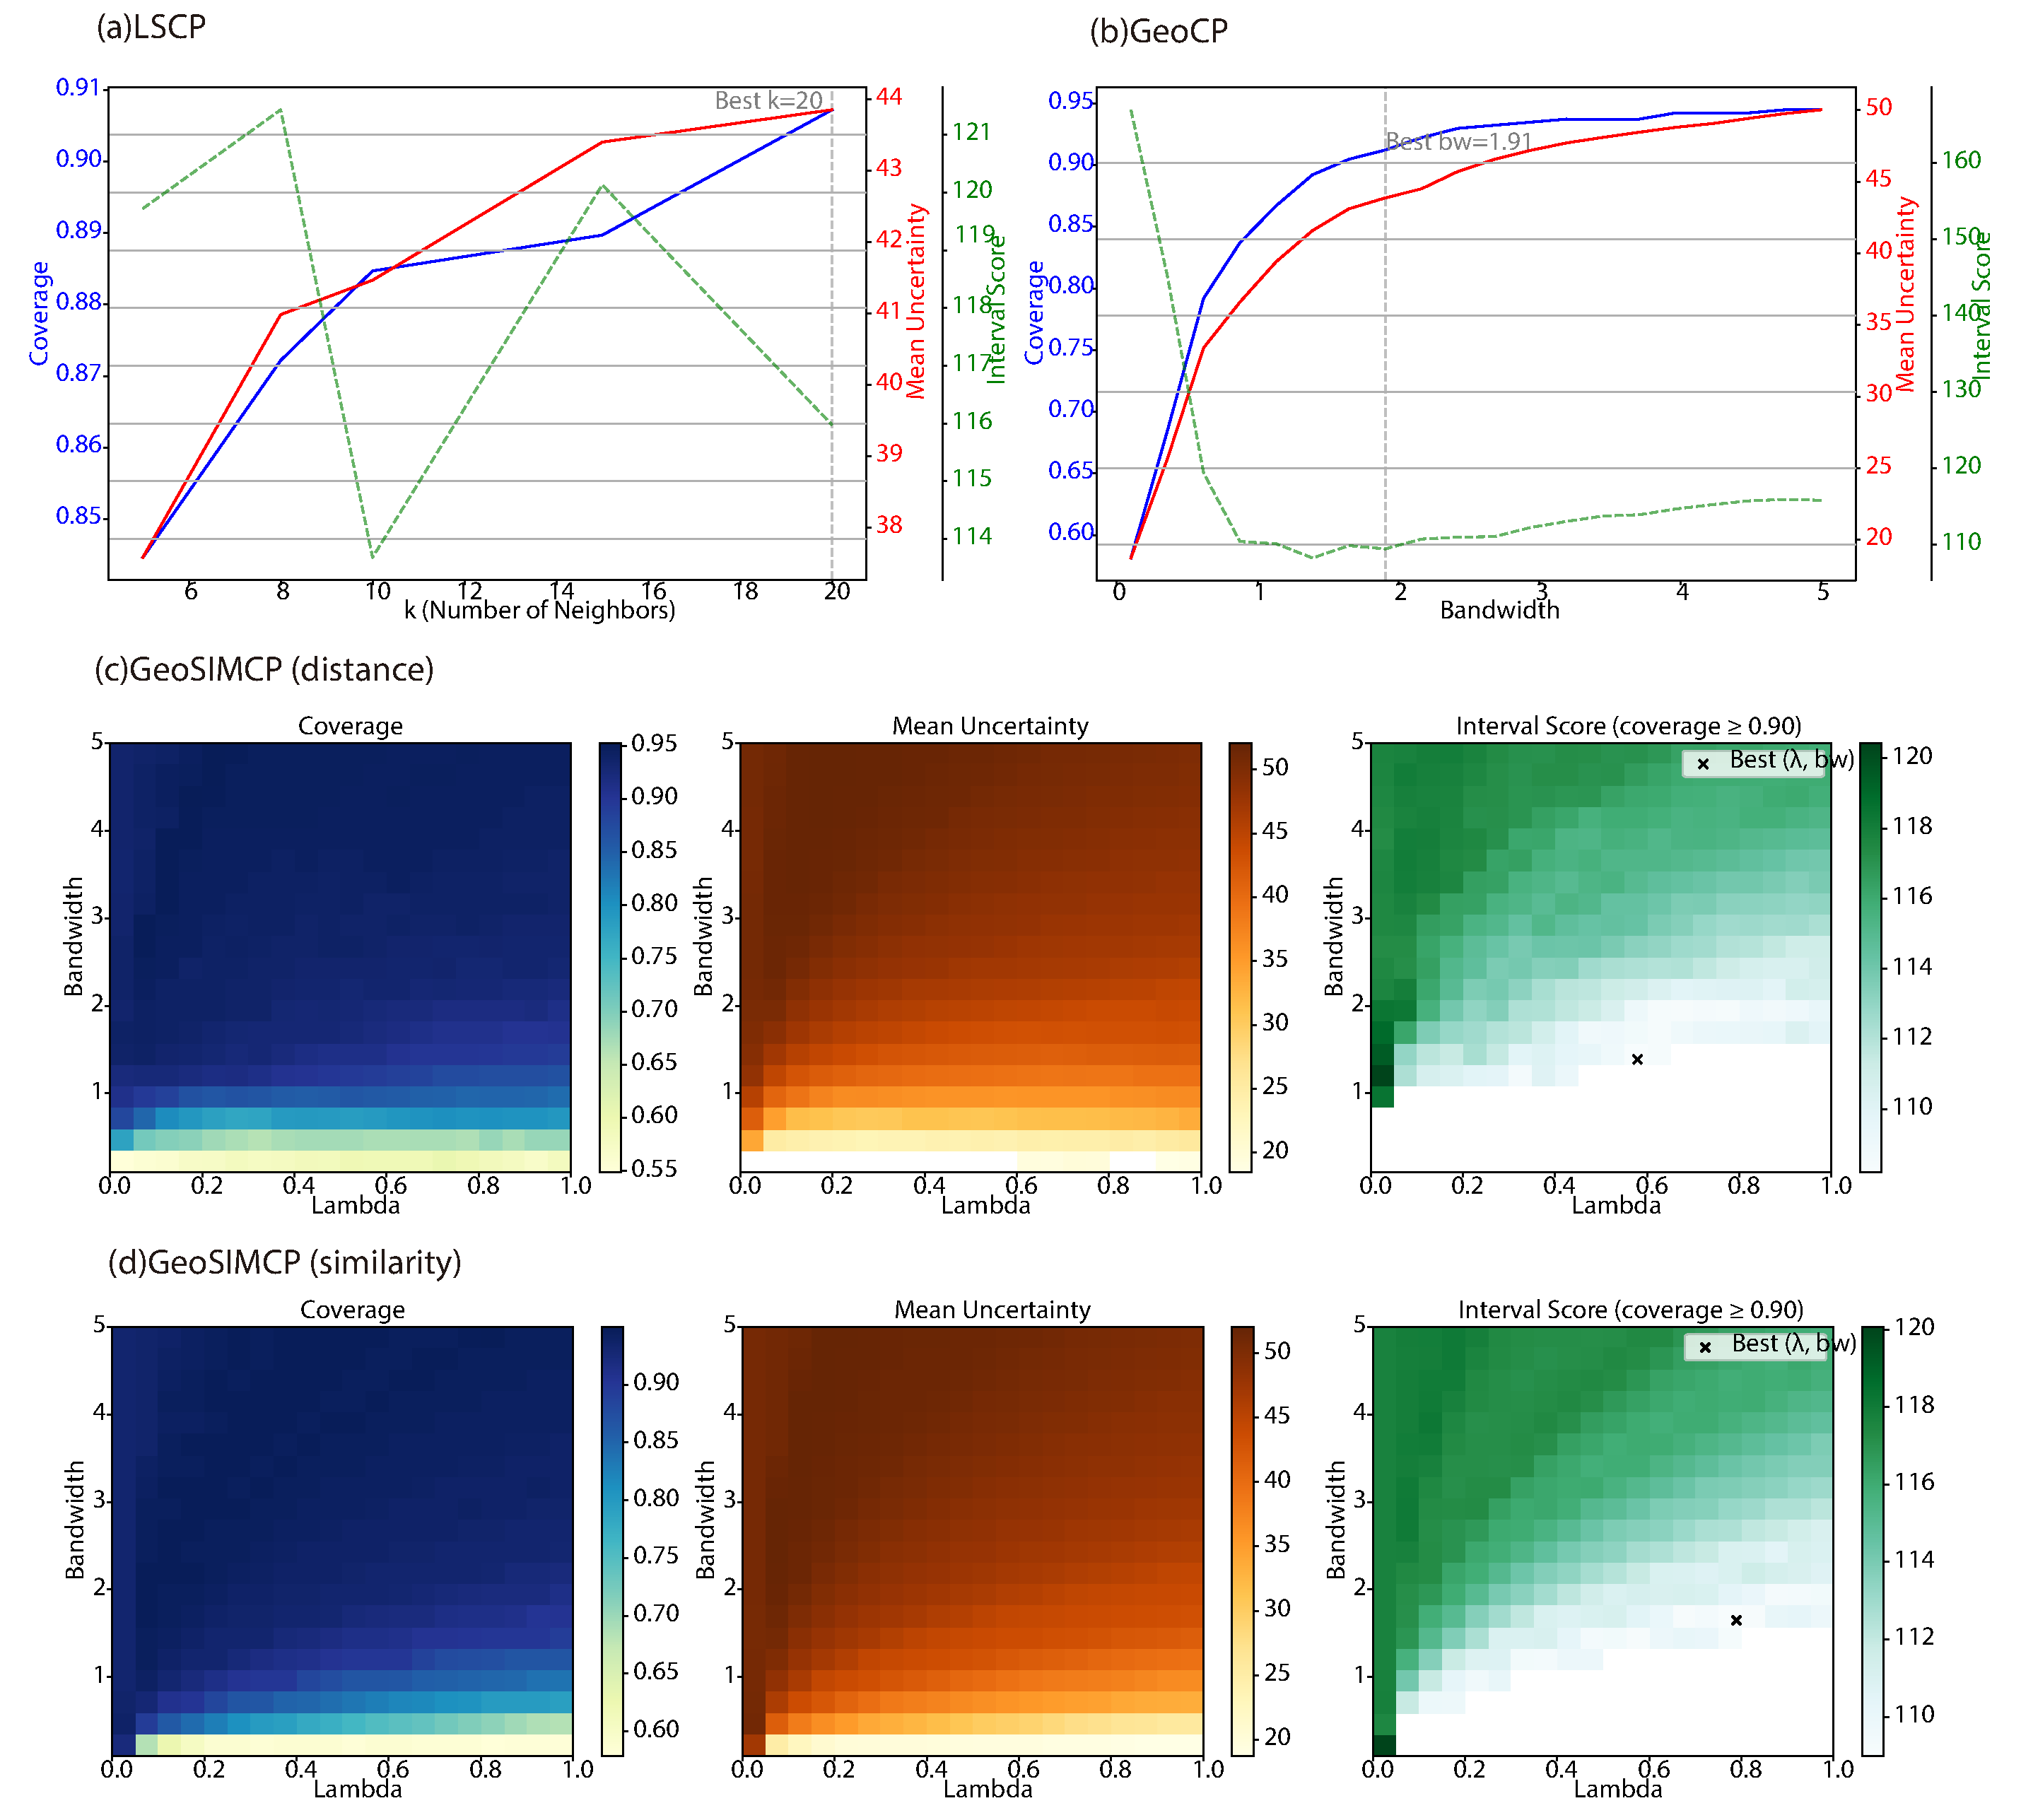
\includegraphics[width=1\linewidth]{Figures/FigureX_Result_USlife.pdf}
%     \caption{Estimating the expectation value of explanation output}
%     \label{fig:framework_mlp}
% \end{figure*}



\begin{figure*}[htbp]
    \centering
    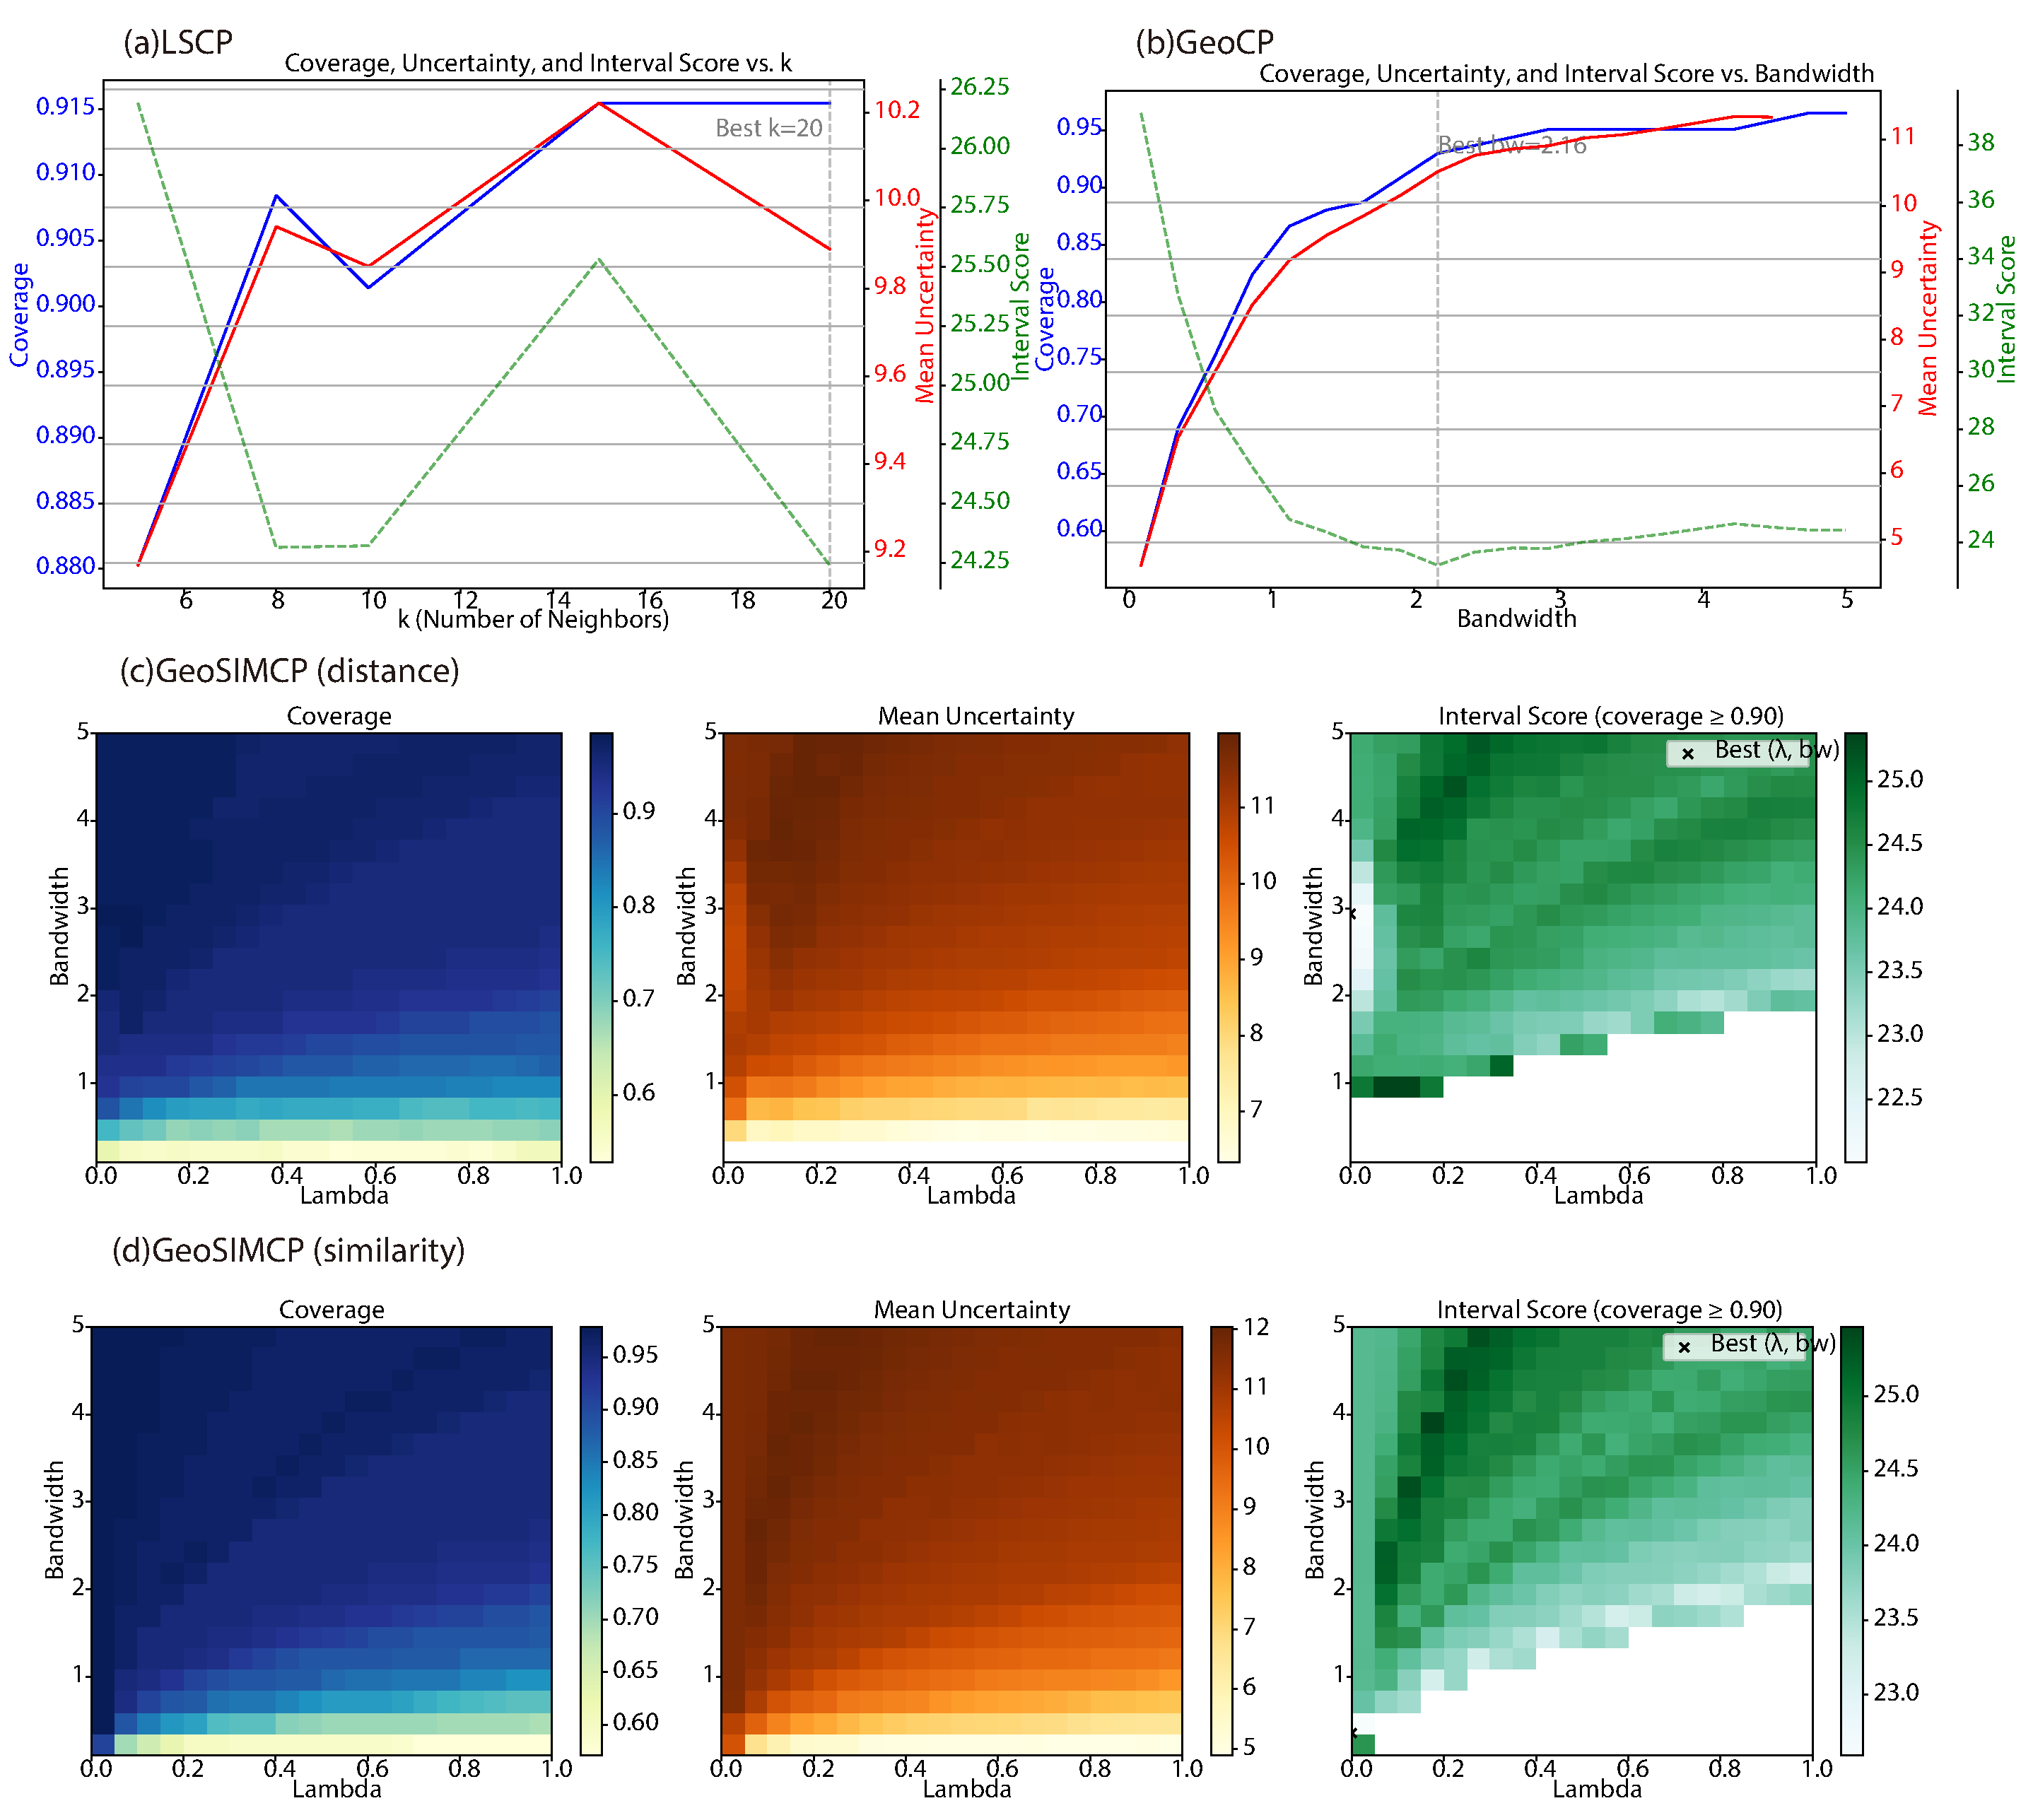
\includegraphics[width=1\linewidth]{Figures/FigureX_Result_PM2.5.pdf}
    \caption{Parameter optimization of these models in the tasks of PM2.5 prediction in China}
    \label{fig:appendix-pm2.5}
\end{figure*}


\begin{figure*}[htbp]
    \centering
    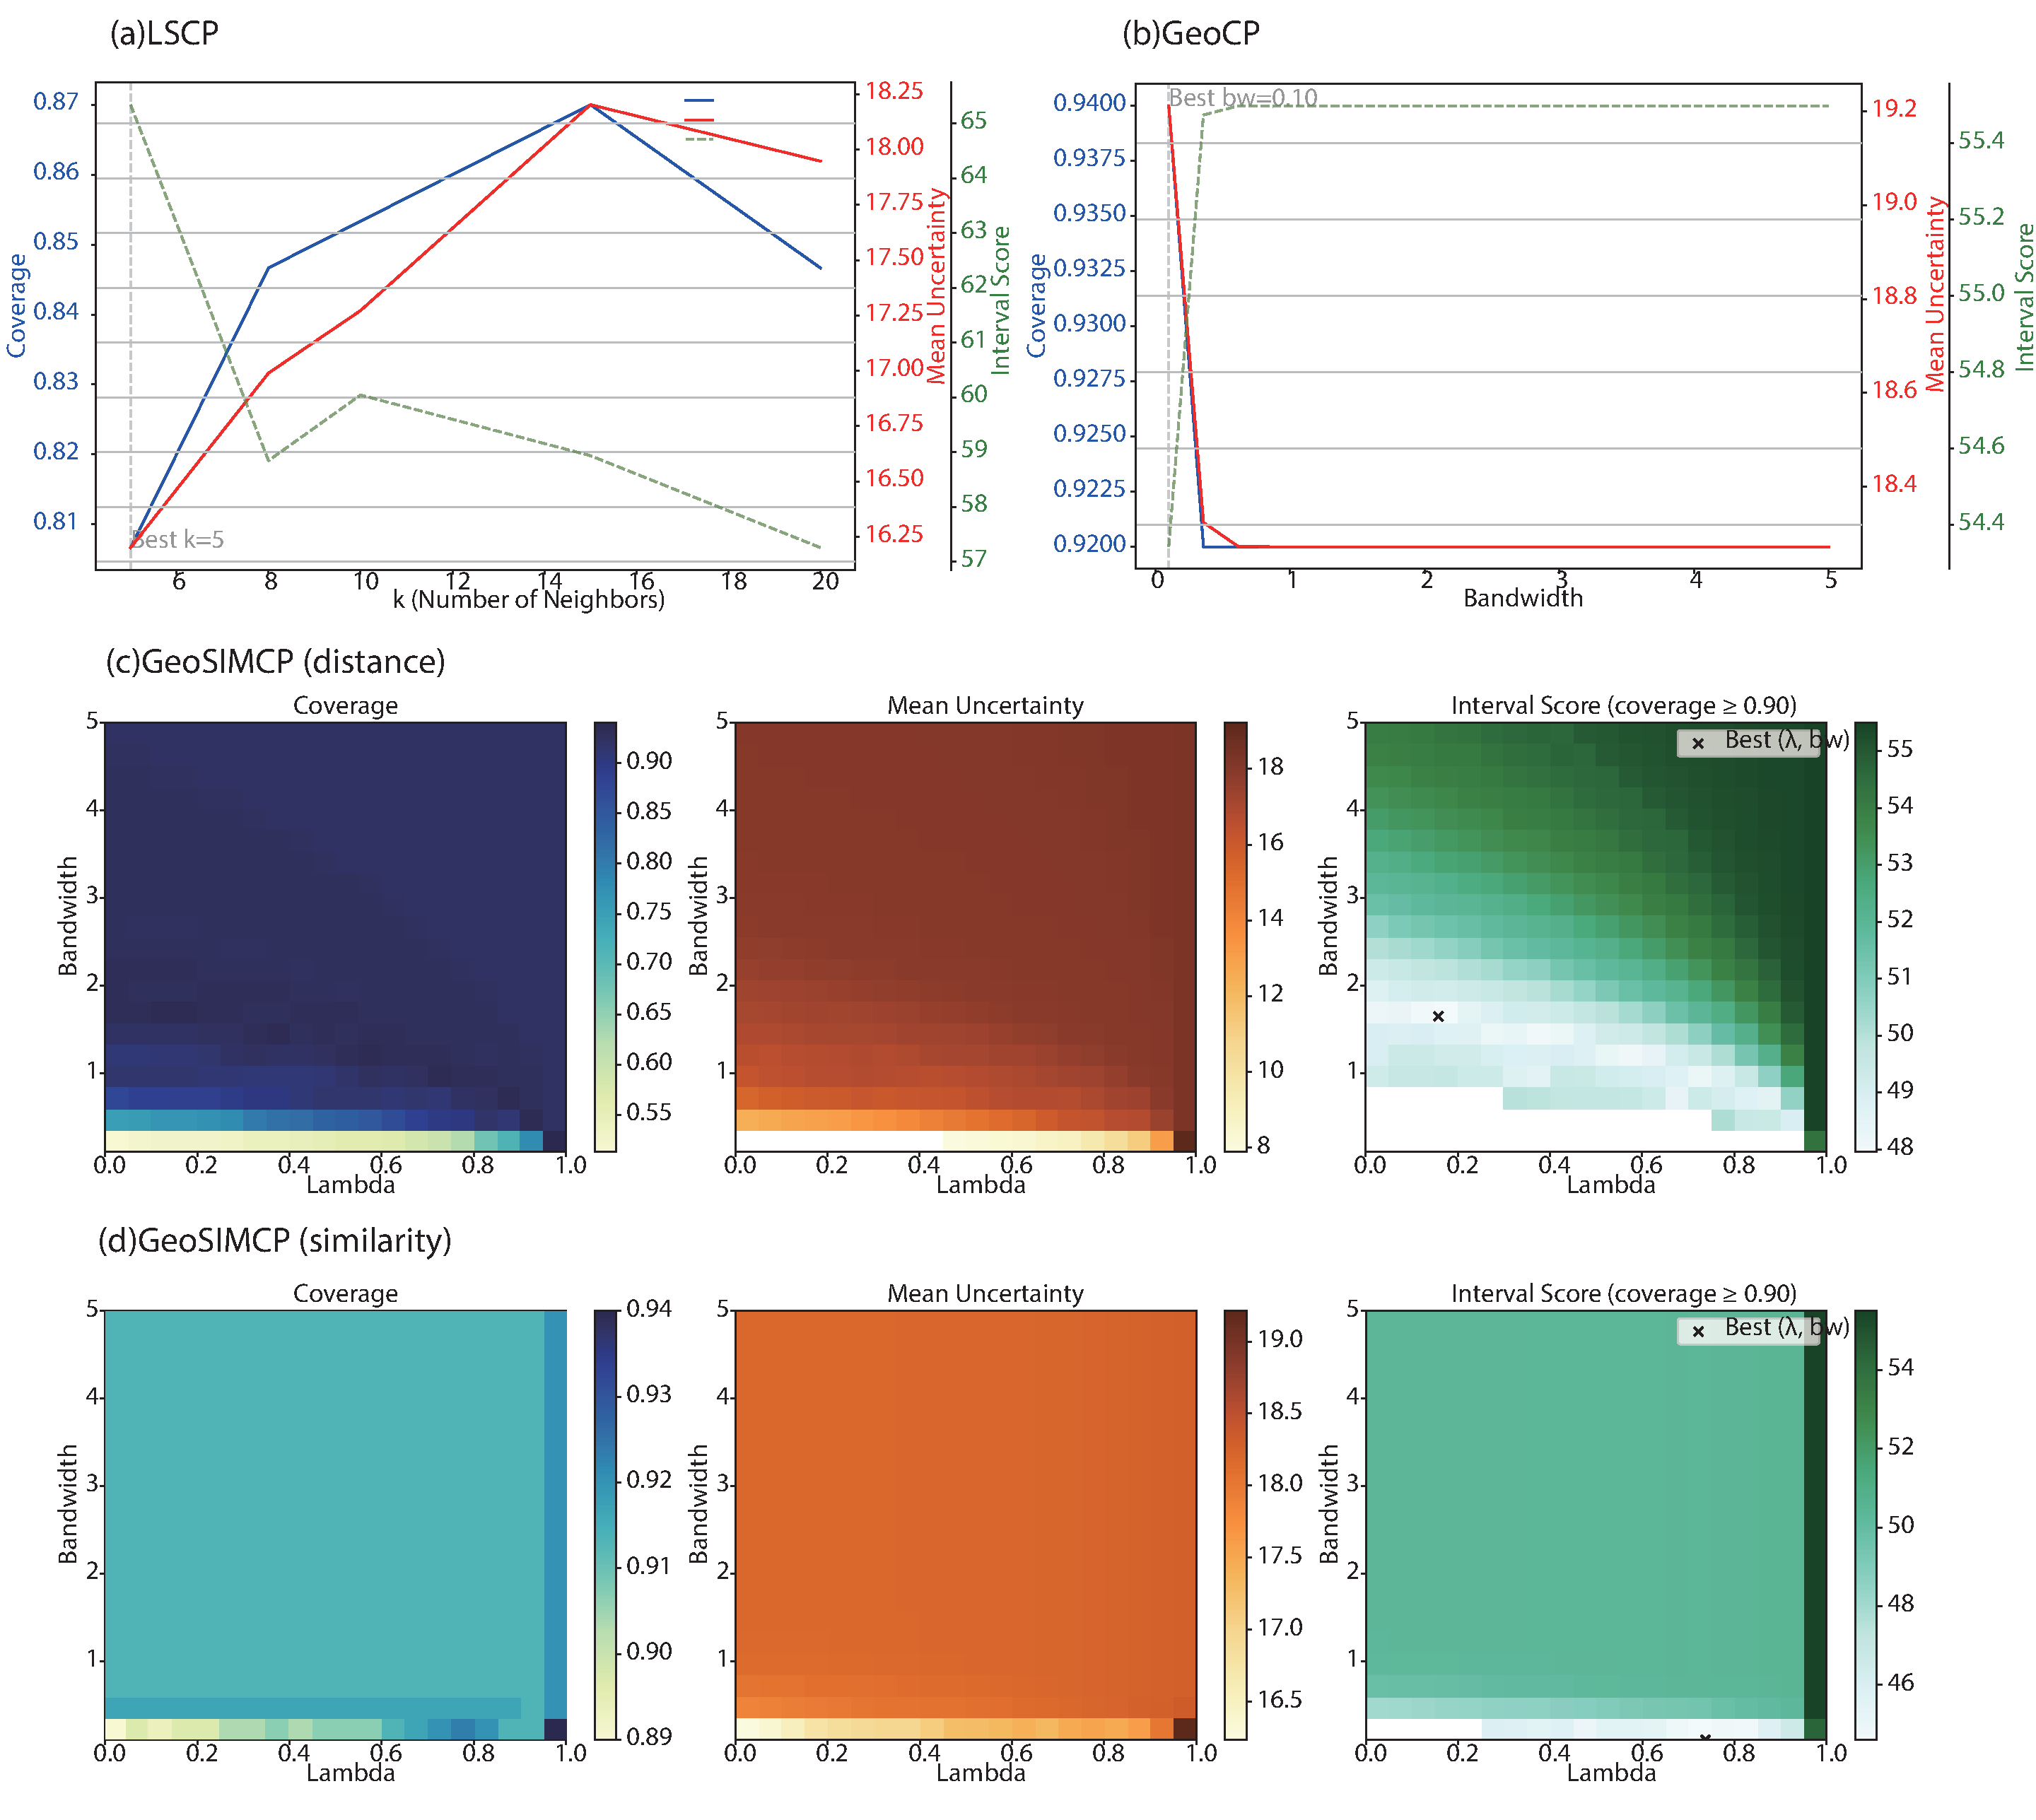
\includegraphics[width=1\linewidth]{Figures/FigureX_Result_housing.pdf}
    \caption{Parameter optimization of these models in the tasks of housing price prediction in Seattle}
    \label{fig:appendix-housing}
\end{figure*}


%\section*{References}
\baselineskip12pt
\bibliographystyle{elsarticle-harv} 
\bibliography{02_references.bib} 


%%%%%%%%%%%%%%%%%%%%%%%%%%%%%%%%%%%%%%%%%%%%%%%%%%%





\end{document}
